\documentclass{uscthesis}

%%%%%%%%%%%%%%%%%%%%%%%%%%%%%%%%%%%%%%%%%%
%%% Options include: [forbinding], which produces 
%%% an alternative title page and an appropriate
%%% binding margin,  [honors] for Honors College theses,
%%% and [durt] for undergraduate thesis submitted as part
%%% part of the distinction in mathematics program.
%%%%%%%%%%%%%%%%%%%%%%%%%%%%%%%%%%%%%%%%%%

%%%%%%%%%%%%%%%%%%%%%%%%%%%%%%%%%%%%%%%%%%
%%  LaTeX Preamble
%%%%%%%%%%%%%%%%%%%%%%%%%%%%%%%%%%%%%%%%%%


\usepackage{style}

%%%%%%%%%%%%%%%%%%%%%%%%%%%%%%%%%%%%%%%%%%
%% You should include above
%% any LaTeX packages that you need.  Most packages should work 
%% with this documentclass.
%%%%%%%%%%%%%%%%%%%%%%%%%%%%%%%%%%%%%%%%%

\usepackage[style=uscauthoryear]{biblatex}
\bibliography{bib/references}
%\usepackage[author-year]{uscamsrefs}

%%%%%%%%%%%%%%%%%%%%%%%%%%%%%%%%%%%%%%%%
%% The lines above specify a BibTeX style which controls 
%% the appearance of the bibliography and how citations to
%% the bibliography within the text will work.  It is based on the biblatex.sty
%% package and provides a Chicago style, as preferred by the Graduate School.
%% There are other acceptable styles.  Indeed, different academic disciplines
%% have different styles.
%% 
%% The line  \bibliography{references} will cause LaTeX is search for a file
%% called references.bib.  This file could be named differently.  For example
%% \bibliography{henry} would provoke a search for henry.bib.  The
%% file reference.bib (or henry.bib) is one you will have to produce.  It is
%% a BibTeX database of references you use.
%% 
%% There are a number of alternate ways to address your bibliographic needs.
%% See the documentation uscthesisdoc.pdf  for a discussion of the different options.
%%
%%
%% 
%%In any case, this  is a good spot to ask LaTeX to load what it needs to handle
%% literature citations and to layout the bibliography. 
%%
%%%%%%%%%%%%%%%%%%%%%%%%%%%%%%%%%%%%%%%%%%


%%%%%%%%%%%%%%%%%%%%%%%%%%%%%%%%%%%%%%%%%%%%
%%  These are just a few sample lines. Put here any 
%%  commands of your own devising that you want to use.
%%  If these examples are no use to you, omit them.
%%%%%%%%%%%%%%%%%%%%%%%%%%%%%%%%%%%%%%%%%%%%%


%%%%%%%%%%%%%%%%%%%%%%%%%%%%%%%%%%%%%%%%%%%%%%%%%%%%%%
%%             The Front Matter
%%  The section below deals with the material that comes 
%%  before the actual content of the document: The title 
%%  page, abstract, acknowledgments,etc.
%%
%%  Some of it is required.
%%%%%%%%%%%%%%%%%%%%%%%%%%%%%%%%%%%%%%%%%%%%%%%%%%%%%%

\title{Geometry of Derived Categories on Noncommutative Projective Schemes}

\author{Blake Alexander}{Farman}    %% First Name then 
                                 %% Last Name

\degreedate{2018}                      %% The year of graduation

%\month{December}                 %% Only for the honors option
                                 %% where it is REQUIRED

\otherdegrees{
Bachelor of Science\\
Rensselaer Polytechnic Institute 2009\\ [\baselineskip]
Master of Science\\
University of Vermont 2011\\ %% The \\ on this line is 
}                                %% ESSENTIAL!

\degreename{Doctor of Philosophy}     %% The Graduate School provides 
                                 %% a list of official degrees.
\field{Mathematics}              %% Fields also provided by the 
                                 %% Graduate School.
\college{College of Arts and Sciences}  %%As listed by Grad School

\advisor {Dr.}{Matthew R. Ballard}{Major Professor}  %%% Be sure the 
\readera{Dr.}{Frank Thorne}{Committee Member}     %%% third field is 
\readerb{Dr.}{Jesse Kass}{Jazzman}          %%% the one used in 
\readerc{Dr.}{Andrew Kustin}{Fourth Reader} %%% your department.
\readerd{Dr.}{Michael Filaseta}{King}               %%% Only use as many as
%%% If you have just two readers, for example, leave out \readerc and
%%% \readerd
%%%
%%% For Honors College theses use \reader{}{}   NO third field.
%%% The commands \otherdegrees, \degree, \field, \college, \readera, etc.
%%% are not used under the honors option.
%%%%%%%%%%%%%%%%%%%%%%%%%%%%%%%%%%%%%%%%%%%%%%%%%%%%%%%

\dean{Dr. Cheryl Addy}{Vice Provost and Dean of the Graduate School}   %% The Dean of the Graduate School
                   %% BE SURE TO CHECK THE NAME OF THE
                   %%PERSON CURRENTLY HOLDING THIS POSITION	
		   %% and the correct title.		             		
                     %% For Honors College theses use
                     %% \schcsigner{}{}.  For example,
                     %% \schcsigner{Dr.}{Davis Baird}

\copyrightpage       %% This is optional. It makes a 
                     %% copyright page that will appear 
                     %% immediately after the title page.

\abstract{FrontMatter/abstract}  %% This calls the file herkimer.tex but 
                     %% but you might replace herkimer by 
                     %% anything you like, for example by 
                     %% abstract. Note, the Graduate School
                     %% REQUIRES that PhD dissertations have 
                     %% abstracts.
                     %%
                     %% For Honors College theses use
                     %% \honorsabstract{}

%\summary{precis}     %% This command calls  precis.tex
                     %% It is only available with the honors
                     %% option and it is REQUIRED for Honors
                     %% theses. 

\acknowledgments{FrontMatter/thanks} %% This calls the file thanks.tex 
%% This is optional       %% where you have put your 
                          %%acknowledgments.

\dedication{FrontMatter/dedication}   %% Calls dedication.tex
%%% Also optional

\preface{FrontMatter/preface}    %% Calls forward.tex.  Optional.

%\makeLoT               %% Issue this command if your work has 
                       %% four or more tables.  A list of tables 
                       %% will be produced automatically.

%\makeLoF               %% works the same way but for figures.

%%%%%%%%%%%%%%%%%%%%%%%%%%%%%%%%%%%%%%%%%%%%%%%%%%%%%%%%%%%%
%%  Finally, here is the meat.  The idea is to compose a 
%%  .tex file for each section of your thesis or dissertation.  
%%  Then use LaTeX's \include command to put them all together.  
%%  Doing it this way makes it easier to change the order of 
%%  exposition as your writing is in progress.  Also it
%%  makes it easy to print out just one section. The \include
%%  command always starts a new page. So every section would 
%%  start on a new page.  If you would like for sections just
%%  to continue, after the appropriate vertical space, on the
%%  current page, then use the \input command instead of the 
%%  \include command.
%%%%%%%%%%%%%%%%%%%%%%%%%%%%%%%%%%%%%%%%%%%%%%%%%%%%%%%%%%%%

\begin{document}

\chapter*{Introduction}
One of the most useful and pleasing statements in algebra is the Morita Theorem \parencite{Morita}.

\begin{theorem}
  Let \(A\) and \(B\) be rings and assume we have an equivalence of module categories 
  \begin{displaymath}
    F : \Mod{A} \to \Mod{B}.
  \end{displaymath}
  Then there exists an \(A\)-\(B\) bimodule which is projective as an \(A\)-module and isomorphic to \(B\) as a \(B\)-module. Consequently, \(P \otimes_A -\) is an equivalence. 
\end{theorem}

For noncommutative rings, one can easily find non-isomorphic examples of Morita equivalent rings.
One such easy example is the equivalence between the modules over a ring \(A\) and the modules over its matrix ring, \(\op{M}_n(A)\), given by the bimodule \(A^n\).
For commutative rings, two rings are Morita equivalent if and only if they are isomorphic. One can try to slacken the relationship by considering the derived version of Morita for rings \parencite{Rickard}.

\begin{theorem}
  Let \(A\) and \(B\) be rings and assume we have an equivalence of derived categories of modules
  \begin{displaymath}
    F : \mathrm{D}(\Mod{A}) \to \mathrm{D}(\Mod{B}).
  \end{displaymath}
  Then there exists a complex of \(A\)-\(B\) bimodules which is perfect as a complex of \(A\)-modules and whose derived endomorphisms as \(B\)-modules are just \(B\) in degree \(0\). Consequently, \(P \overset{\mathbf{L}}{\otimes}_A -\) is an equivalence. 
\end{theorem}

Even still, here two commutative rings are derived Morita equivalent if and only if they are isomorphic. To get a strictly weaker equivalence relation, we should globalize the notion of a commutative ring by passing to schemes. 

\begin{theorem}
  Let \(X\) and \(Y\) be quasi-compact, quasi-separated schemes over a field, \(k\), and assume we have an equivalence 
  \begin{displaymath}
    F: \mathrm{D}(\Qcoh{X}) \to \mathrm{D}(\Qcoh{Y}).
  \end{displaymath}
  Then there exists an object \(P \in \mathrm{D}(\Qcoh{X \times Y})\) such that
  \begin{displaymath}
    M \mapsto \Phi_P (M) := \mathbf{R}\pi_{Y \ast} \left( P \overset{\mathbf{L}}{\otimes} \mathbf{L}\pi_X^\ast M \right) 
  \end{displaymath}
  gives an equivalence. 
\end{theorem}

Here \(X \overset{\pi_X}\longleftarrow X \times Y \overset{\pi_Y}\longrightarrow Y\) are the projections. This result, as stated, follows immediately from results of T\"oen and Lunts-Orlov \parencite{Toen07,Lunts-Orlov}. A more specific version for smooth projective schemes predates this \parencite{Orlov97}. In this generality, we unlock a deep and subtle equivalence relationship. Indeed, understanding these Fourier-Mukai partnerships is a central problem in the field of derived categories in algebraic geometry. 
Given the richness of the globalized Morita statement for commutative rings, one is led to think about a globalized version for noncommutative rings. A framework for phrasing such a question is due to Artin and Zhang \parencite{AZ94} and goes by the name Noncommutative Projective Geometry. A graded Morita theorem for noncommutative rings is due to Zhang \parencite{Zhang96}.  


Following the line of thought above, one wonders about derived Morita theory for noncommutative projective schemes \(X\) and \(Y\) which are associated to connected graded \(k\)-algebras \(A\) and \(B\).
As an application of the main result of this article, we have the following statement. One says that \(A\) and \(B\) form a delightful couple if they are both Ext-finite in the sense of \parencite{VdB}, both are left and right Noetherian, and both satisfy \(\chi^\circ(R)\) for \(R=A,A^\opp\) for \(A\) and \(R = B, B^\opp\) for \(B\). One can think of this requirement as Serre vanishing for the twisting sheaves plus some finite-dimensionality over \(k\).

\begin{theorem}
  Let \(X\) and \(Y\) be noncommutative projective schemes associated to a delightful couple of over a field \(k\), both of which are generated in degree one.
  Then for any equivalence \(\mathrm{D}(\Qcoh{X}) \to \mathrm{D}(\Qcoh{Y})\), there exists an object \(P\) of \(\mathrm{D}(\Qcoh{X \times_k Y})\) whose associated integral transform is an equivalence of Fourier-Mukai type.
\end{theorem}

\noindent
The interested reader can see Corollary~\ref{corollary: NCP morita degree 1} for a more careful statement of this result.

This result is, as the notation suggests, an application of a more general result. Work of T\"oen provides a good bicategorical structure for dg-categories up to quasi-equivalence \parencite{Toen07} - an internal Hom. The construction of \(\RHomc{\mathcal C, \mathcal D}\) is abstract even if the dg-categories \(\mathcal C\) and \(\mathcal D\) arise geometrically (or noncommutative geometrically). To unleash the power of T\"oen's work, one needs to identify the internal Hom more ``internally.'' Indeed, this is done for schemes in \parencite{Toen07}, for higher derived stacks (using machinery of Lurie in place of T\"oen) in \parencite{BFN10}, and matrix factorizations in \parencite{Dyckerhoff11,PV12,BFK14}. The main result here is the identification of this internal Hom in Noncommutative Projective Geometry, see Theorem~\ref{theorem: derived morita for NCP}. 

%TODO: Try to fit the stuff down here and the stuff above together, coherently.
\subsection*{Fourier-Mukai Kernels for Noncommutative Projective Schemes}

In light of their absense in noncommutative projective geometry, the natural question to ask is what these kernels should be.
To\"en's derived Morita theory \parencite{Toen07} gives an overarching framework to attack such a problem by abstracting to the higher categorical structure of differential graded (dg) categories.
Working within the homotopy category of the 2-category of all small dg-categories over a commutative ring, To\"en is able to provide an incredibly elegant reformulation of Fourier-Mukai functors at the level of pre-triangulated dg-categories via the dg-subcategory, \(\mathbb{R}\underline{\operatorname{Hom}}_c\), of the internal Hom.
Indeed, using this machinery, kernels have been recovered for schemes in \parencite{Toen07}, and obtained for higher derived stacks in \parencite{BFN10} and for categories of matrix factorizations in \parencite{Dyckerhoff11,PV12,BFK14}.
In each case, the work lies in the identification of the internal Hom object obtained from this machinery within the theory from which the input dg-categories originate, for even if they arise geometrically, the resulting Hom is often quite abstract.

The obvious first step in such work is to identify the possible input dg-categories for the machinery of derived Morita theory.
In the situation of interest, one considers the noncommutative projective scheme, \(\operatorname{QGr} A\), associated to the connected graded algebra, \(A\), over a field, \(k\). 
The natural choice of dg-category is the dg-enhancement, \(\mathcal{D}(\operatorname{QGr} A)\), of the derived category \(\operatorname{D}(\operatorname{QGr} A)\), in the sense of \parencite{Lunts-Orlov}, which is unique up to equivalence in the homotopy category of dg-categories.
One must then identify the dg-category \(\mathbb{R}\underline{\operatorname{Hom}}_c(\mathcal{D}(\operatorname{QGr} A), \mathcal{D}(\operatorname{QGr} B))\) noncommutative geometrically.

Generally, care must be taken to ensure good behavior of \(\operatorname{QGr} A\), but one may exert some control by imposing cohomological conditions on the ring, \(A\).
Two such common conditions are the Ext-finite condition of \parencite{BVdB} and the condition \(\chi^\circ(M)\) of \parencite{AZ94}.
One can interpret these conditions geometrically as imposing Serre vanishing for the noncommutative twisting sheaves together with a local finite dimensionality over the ground field, \(k\).
Specifically, one can force good behavior with respect to To\"en's derived Morita theory by requiring that two connected graded algebras, \(A\) and \(B\), over a field, \(k\), are both left and right Noetherian, Ext-finite, and satisfy the condition \(\chi^\circ(M)\) for the left/right \(A\)-modules \(M = A, A^{\operatorname{op}}\), and the left/right \(B\)-modules \(M = B, B^{\operatorname{op}}\).

In this work we establish the identification
\[\mathbb{R}\underline{\operatorname{Hom}}_c(\mathcal{D}(\operatorname{QGr} A), \mathcal{D}(\operatorname{QGr} B)) \cong \mathcal{D}(\operatorname{QGr}(A^{\operatorname{op}} \otimes_k B))\]
in the homotopy category of dg-categories under these hypotheses.
As an easy corollary, a pleasing derived Morita statement is obtained.
\begin{theorem}
  If there exists an equivalence
  \(f \colon \operatorname{D}(\operatorname{QGr} A) \to \operatorname{D}(\operatorname{QGr} B)\),
  then there exists an object \(P\) of \(\operatorname{D}\left(\operatorname{QGr} \left(A^{\operatorname{op}} \otimes_k B\right)\right)\) and a Fourier-Mukai transform
  \(\Phi_P \colon \operatorname{D}(\operatorname{QGr} A) \to \operatorname{D}(\operatorname{QGr} B)\)
  that is an equivalence.
\end{theorem}

\section*{Conventions}
The ring \(k\) will always be Noetherian and commutative.
Often, for ease of notation, \(\C(X,Y)\) will be used to refer to the morphims, \(\op{Hom}_\C(X,Y)\), between objects \(X\) and \(Y\) of a category \(\C\). We shall also use an undecorated \(\op{Hom}\) depending on the complexity of the notation. 
Whenever \(\C\) has a natural enrichment over a category, \(\mathcal{V}\), we will denote by \(\underline{\C}(X,Y)\) the \(\mathcal{V}\)-object of morphisms.

For example, the category of complexes of \(k\)-vector spaces, \(\Ch{k}\), can be endowed with the the structure of a \(\Ch{k}\)-enriched category using the hom total complex, \(\CH{k}(C,D) := \underline{C}(k)(C,D)\) which has in degree \(n\) the \(k\)-vector space
\[\CH{k}(C,D)^n = \prod_{m \in \Z}\Mod{k}\left(C^m, D^{m + n}\right)\]
and differential
\[d(f) = d_D \circ f + (-1)^{n+1} f \circ d_C.\]
It should be noted that \(Z^0(\CH{k}(C,D)) = \Ch{k}(C,D)\).
    %% Calls Introduction.tex
                          %% Honors theses are required to 
                          %% have an Introduction.  For
                          %% Honors theses, the file 
                          %% Introduction.tex should begin
                          %%
                          %% \chapter*{Introduction}
                          %% followed by the text of the 
                          %% introduction.

\documentclass[dissertation.tex]{subfiles}
\begin{document}
\section{Differential Graded Modules and Algebras}
{\noindent Throughout, let $k$ be a commutative ring.}

\begin{defn}
  A {\it differential graded $k$-module}, $M$, is a complex of $k$-modules
  $$M \colon \begin{tikzcd}
    \cdots \arrow{r}{d_M^{n-2}} & M^{n-1} \arrow{r}{d_M^{n-1}} & M^n \arrow{r}{d_M^n} & M^{n+1} \arrow{r}{d_M^{n+1}} & \cdots
  \end{tikzcd},$$
  or, equivalently, a $\Z$-graded module over the graded ring $k$, concentrated in degree 0, equipped with a degree one morphism $d_M : M \rightarrow M[1]$ such that $d_M^2 = 0$.
  A {\it morphism of differential graded $k$-modules} is a morphism of chain complexes.
  
  The {\it shift} of a dg $k$-module is the shifted complex
  $$M[1] \colon \begin{tikzcd}
    \cdots \arrow{r}{-d_M^{n-1}} & M^{n} \arrow{r}{-d_M^{n}} & M^{n+1} \arrow{r}{-d_M^{n+1}} & M^{n+2} \arrow{r}{-d_M^{n+2}} & \cdots
  \end{tikzcd}$$
  
  The tensor product of two dg $k$-modules is the usual tensor product in $\Ch{k}$, the category of chain complexes of $k$-modules.
\end{defn}

\begin{defn}
  We say a category, $\CC$, is a {\it $k$-category} if
  \begin{enumerate}
  \item
    for each pair of objects $X$ and $Y$ of $\CC$, $\Hom{\CC}{X,Y}$ is a $k$-module, and
  \item
    composition 
    $$\Hom{\CC}{X,Y} \otimes_k \Hom{\CC}{Y,Z} \rightarrow \Hom{\CC}{X,Z}$$
    in $\CC$ is $k$-linear, associative, admitting units $\id_X \in \Hom{\CC}{X,X}$.
  \end{enumerate}
\end{defn}

\section{The Category of Differential Graded Categories}

\begin{defn}
  A {\it differential graded} or {\it dg category} is a $k$-category, $\CC$, satisfying
  \begin{enumerate}
  \item
    $\Hom{\CC}{X,Y}$ is a dg $k$-module for all objects $X,Y$ of $\CC$, and
  \item
    composition 
    $$\begin{tikzcd}
      \Hom{\CC}{X,Y} \otimes_k \Hom{\CC}{Y,Z} \arrow{r} & \Hom{\CC}{X,Z}
    \end{tikzcd}$$
    in $\CC$ is a morphism of dg $k$-modules;
    that is a morphism of $\Ch{k}$.
  \end{enumerate}
  
  A {\it morphism of dg categories}, or {\it dg functor}, $\mathscr{F} \colon \CC \rightarrow \D$, is a functor such that
  $$F(X,Y) \colon 
  \begin{tikzcd}
    \Hom{\CC}{X,Y} \arrow{r} & \Hom{\D}{FX,FY}
  \end{tikzcd}$$
  is a morphism of dg $k$-modules.
  Denote by $\operatorname{dgcat}_k$ the category with objects small dg categories and morphisms dg functors.
\end{defn}

\begin{eg}
  \begin{description}[style=nextline]
  \item[dg category with one object]
    Let $A$ be a dg $k$-algebra; that is, a graded $k$-algebra equipped with a differential
    $$d(fg) = d(f)g + (-1)^nfd(g),\ f \in A^n, g \in A.$$
    Define $\mathscr{A}$ to be the category with one object, $\ast$, and morphisms $\mathscr{A}(\ast, \ast) = A$, with composition defined by the multiplication in $A$.
  \item[dg $k$-modules]
    Define the category $\mathcal{C}_\text{dg}(k)$ to have objects chain complexes of $k$-modules, and morphisms $\mathcal{C}_\text{dg}(k)(C,D) = [C,D]_{\Ch{k}}$, the internal hom for $\Ch{k}$ as in Definition~\ref{ChInternalHomDefn}.
    The composition of morphisms
    $$\begin{tikzcd}
      \cdg{k}(C,D) \otimes_k \cdg{k}(D,E) \arrow{r} & \cdg{k}(C,E)
    \end{tikzcd}$$
    is the composition morphism of Remark~\ref{MorphismsOfDGModules} (\ref{MorphismsOfDGModules.composition}).
    
    As an immediate consequence of Proposition~\ref{ChHomTensorAdjunction} we have the following observation:
    \begin{prop}
      %The category $\mathcal{C}_\text{dg}(k)$ is both a tensored and cotensored $\Ch{k}$-category.
      For any three chain complexes, $C$, $D$, and $E$, there is a canonical isomorphism of chain complexes
      $$\cdg{k}(C \otimes_k E, D) \cong \cdg{k}(C,\cdg{k}(E,D)).$$
      
      \begin{proof}
        Let $X$ be any object of $\Ch{k}$.
        Using the adjunction of Proposition~\ref{ChHomTensorAdjunction} we have
        \begin{eqnarray*}
          \Ch{k}(X,\cdg{k}(C \otimes_k E, D) &\cong& 
          \Ch{k}(X \otimes_k (C \otimes_k E), D)\\
          &\cong& \Ch{k}((X \otimes_k C) \otimes_k E, D)\\
          &\cong& \Ch{k}(X \otimes_k C, \cdg{k}(E,D))\\
          &\cong& \Ch{k}(X, \cdg{k}(C, \cdg{k}(E,D)).
        \end{eqnarray*}
        Therefore by the Yoneda Lemma there is a unique isomorphism 
        $$\cdg{k}(C \otimes_k E, D) \cong \cdg{k}(C, \cdg{k}(E,D)).$$
      \end{proof}
    \end{prop}
    %Note that $[C,D]$ is, equivalently, the graded module of graded morphisms; that is, a morphism $f \in \mathcal{C}_\text{dg}(k)(C, D)^m$ is a collection of morphisms $f^n \colon C^n \rightarrow D^{n+m}$.
    %Equip $\mathcal{C}_\text{dg}(k)(C, D)$ with the differential
    %$$\begin{tikzcd}
    %  \mathcal{C}_\text{dg}(k)(C, D)^n \arrow{r} & \mathcal{C}_\text{dg}(k)(C, D)^{n+1}\\
    %  f \arrow[mapsto]{r} & d_D \circ f + (-1)^{n+1}f \circ d_C
    %\end{tikzcd}$$
    %and define composition of morphisms by the tensor product in $\mathcal{C}(k)$,
    %$$\begin{tikzcd}
    %  \mathcal{C}_\text{dg}(k)(D, E) \otimes_k \mathcal{C}_\text{dg}(k)(C, D) \arrow{r} & \mathcal{C}_\text{dg}(k)(C, E).
    %\end{tikzcd}$$
  \end{description}
\end{eg}

\begin{defn}
  Let $\CC$ and $\D$ be objects of $\operatorname{dgcat}_k$.
  The {\it tensor product}, $\CC \otimes \D$, is the dg category with objects $\operatorname{ob}\CC \times \operatorname{ob}\D$ and
  morphisms
  $$\begin{tikzcd}
    \Hom{\CC \otimes \D}{(X, Y), (X^\prime, Y^\prime)} = \Hom{\CC}{X,X^\prime} \otimes_k \Hom{\D}{Y,Y^\prime}.
  \end{tikzcd}$$
  For ease of notation, we will denote by $X \otimes Y$ the object $(X,Y)$ of $\CC \otimes \D$.
\end{defn}

\begin{defn}
  Given two dg functors $\mathscr{F},\mathscr{G} \colon \CC \rightarrow \D$, define $\SHom{\mathscr{F},\mathscr{G}}^n$ to be the $k$-module of degree $n$ natural transformations.
  That is, morphisms of functors, $\eta \colon \mathscr{F} \rightarrow \mathscr{G}$ such that for each object $X$ of $\CC$, $\eta(X) \in \Hom{\D}{\mathscr{F}(X),\mathscr{G}(X)}^n$.
\end{defn}

\begin{prop}
  Given a degree $n$ natural transformation $\eta \colon \mathscr{F} \rightarrow \mathscr{G}$, the collection of morphisms
  $$d^n_{\Hom{\D}{\mathscr{F}X, \mathscr{G}X}}\left( \eta(X) \right) \in \Hom{\D}{\mathscr{F}X, \mathscr{G}X}^{n+1}$$
  define a natural transformation of degree $n + 1$ and hence endow $\SHom{\mathscr{F},\mathscr{G}}$ with the structure of a dg $k$-module, where the differential, $d_{\SHom{\mathscr{F},\mathscr{G}}}^n$ sends $\eta$ to this natural transformation.
  
  \begin{proof}
    It's clear that so long as the collection of $d^n_{\D(\F X, \G X)}(\eta(X))$ defines a natural transformation, the resulting sequence
    $$\begin{tikzcd}
      \cdots \arrow{r} & \SHom{\F, \G}^n \arrow{r} & \SHom{\F,\G}^{n+1} \arrow{r} & \cdots
    \end{tikzcd}$$
    will be a complex.
    
    First we note that, by definition, any dg functor necessarily commutes with the differentials:
    $$d_{\D(\mathscr{F}X, \mathscr{F}X^\prime)}\left(\mathscr{F}(f) \right) = \mathscr{F}\left(d_{\CC(X,X^\prime)}(f)\right)$$
    and composition is a morphism of dg $k$-modules, so we have the commutative diagrams
    $$\begin{tikzcd}
      \D(\F X^\prime, \G X^\prime) \otimes_k \D(\F X, \F X^\prime) \arrow{r}\arrow[swap]{d}{d \otimes 1 + 1 \otimes d}& \D(\F X, \G X^\prime)\arrow{d}{d}\\
      \D(\F X^\prime, \G X^\prime) \otimes_k \D(\F X, \F X^\prime)[1] \arrow{r}& \D(\F X, \G X^\prime)[1]
    \end{tikzcd}$$
    and
    $$\begin{tikzcd}
      \D(\G X, \G X^\prime) \otimes_k \D(\F X, \G X) \arrow{r}\arrow[swap]{d}{d \otimes 1 + 1 \otimes d}& \D(\F X, \G X^\prime)\arrow{d}{d}\\
      \D(\G X, \G X^\prime) \otimes_k \D(\F X, \G X)[1] \arrow{r}& \D(\F X, \G X^\prime)[1]
    \end{tikzcd}$$
    For a morphism $f \in \CC(X,X^\prime)$, chasing $\eta(X^\prime) \otimes \F(f)$ and $\G(f) \otimes \eta(X)$ through the diagram gives
    \begin{eqnarray*}
      d(\eta(X^\prime)) \circ \F(f) + \eta(X^\prime) \circ d(\F(f)) 
      &=& d(\eta(X^\prime) \circ \F(f))\\
      &=& d(\G(f) \circ \eta(X))\\
      &=& d(\G(f)) \circ \eta(X) + \G(f) \circ d(\eta(X)).
    \end{eqnarray*}
    By the fact that $\F$,$\G$ commute with differentials and $\eta$ is a natural tranformation, we see
    $$\eta(X^\prime) \circ d(\F(f)) = \eta(X^\prime) \circ \F(d(f)) = \G(d(f)) \circ \eta(X) = d(\G(f)) \circ \eta(X).$$
    Therefore
    $$d(\eta(X^\prime)) \circ \F(f) = \G(f) \circ d(\eta(X)),$$
    as desired.
  \end{proof}
\end{prop}

\begin{defn}
  For two objects $\CC$ and $\D$ of $\operatorname{dgcat}_k$, define the object $\SHom{\CC,\D}$ of $\operatorname{dgcat}_k$ to be the category with objects dg functors $\mathscr{F} \colon \CC \rightarrow \D$ and morphisms $\SHom{\mathscr{F},\mathscr{G}}$.
  
  Given two dg functors $\F,\G \colon \CC \rightarrow \D$, define a {\it morphism of dg functors}, $\eta \colon \F \rightarrow \G$ to be a closed, degree zero natural transformation.
  That is, $\eta \in \SHom{\F, \G}^0$ and its image in $\SHom{\F,\G}^1$ under the differential is zero.
\end{defn}

\begin{rmk}
  There is a natural isomorphism of bifunctors
  $$\Hom{\operatorname{dgcat}_k}{\CC \otimes \D, \mathscr{E}} \cong \Hom{\operatorname{dgcat}_k}{\CC, \SHom{\D,\mathscr{E}}},$$
  which endows $\operatorname{dgcat}_k$ with a symmetric closed monoidal structure.
\end{rmk}

\begin{defn}
  Let $\CC$ be a dg category.
  Define
  \begin{enumerate}
  \item
    the category $Z^0(\CC)$ to be the category with objects those of $\CC$ and morphisms
    $$\Hom{Z^0(\CC)}{X,Y} = Z^0\left(\Hom{\CC}{X,Y}\right),$$
  \item
    the category $H^0(\CC)$ to be the category with objects those of $\CC$ and morphisms
    $$\Hom{H^0(\CC)}{X,Y} = H^0\left(\Hom{\CC}{X,Y}\right),$$
  \item
    the {\it homology category}, $H^\ast(\CC)$, to be the category with objects those of $\CC$ and morphisms 
    $$H^\ast\CC(X,Y) = \bigoplus H^n\CC(X,Y).$$
  \end{enumerate}
\end{defn}

\begin{rmk}\label{DGInducedHomology}
  Note that given a dg functor, $\mathscr{F} \colon \CC \rightarrow \D$, for $X$ and $Y$ objects of $\CC$, 
  $$\mathscr{F}(X,Y) \colon \CC(X,Y) \rightarrow \D(\mathscr{F}X, \mathscr{F}Y)$$
  is a morphism of $\mathcal{C}(k)$ and this immediately implies the diagram
  $$\begin{tikzcd}
    B^n(\CC(X,Y))\arrow{r}{\imath^n}\arrow[bend left]{rr}{\im d^{n-1}}\arrow[dashed]{d}{\exists !B^n(\F(X,Y))} & Z^n(\CC(X,Y)) \arrow{r}{\ker d^n}\arrow[dashed]{d}{\exists !Z^n(\F(X,Y))} & \CC(X,Y)^{n} \arrow{d}{\F(X,Y)}\\
    B^n(\D(\F X,\F Y) \arrow{r}{\imath^n}\arrow[bend right]{rr}{\im d^{n-1}} & Z^n(\D(\F X,\F Y))\arrow{r}{\ker d^n} & \D(\F X,\F Y)^{n}
  \end{tikzcd}$$
  commutes for each $n$.
  Hence $H^n$ induces a functor
  $H^n(\mathscr{F}) \colon H^n(\CC) \rightarrow H^n(\D)$
  with object map\\ $H^n(\mathscr{F})(X) = \mathscr{F}(X)$ and induced arrow map 
  $$\begin{tikzcd}
    0 \arrow{r} & B^n(\CC(X,Y))\arrow{r}{\imath^n}\arrow{d}{B^n(\F(X,Y))} & Z^n(\CC(X,Y)) \arrow{r}{\coker \imath^n}\arrow{d}{Z^n(\F(X,Y))} & H^n(\CC(X,Y)) \arrow[dashed]{d}{\exists !H^n(\F(X,Y))}\arrow{r} & 0 \\
    0 \arrow{r} & B^n(\D(\F X,\F Y) \arrow{r}{\imath^n} & Z^n(\D(\F X,\F Y))\arrow{r}{\coker \imath^n} & H^n(\D(\F X,\F Y)) \arrow{r} & 0
  \end{tikzcd}$$
\end{rmk}

\section{Modules over a Differential Graded Category}

\begin{defn}
  Let $\CC$ be a small dg category and let $\mathscr{M} : \CC \rightarrow \mathcal{C}_\text{dg}(k)$ be a dg functor.
  \begin{enumerate}
  \item
    We say that $\mathscr{M}$ is a right (resp. left) dg $\CC$-module if $\mathscr{M}$ is contravariant (resp. covariant).
  \item
    The {\it homology of a dg $\CC$-module}, $\mathscr{M}$, is the induced functor
    $$\begin{tikzcd}
      H^\ast(\CC) \arrow{r}{H^\ast(\mathscr{M})}& \Gr{k}\\
      X \arrow[mapsto]{r} & H^\ast(\mathscr{M}(X))
      %H^\ast(\CC(Y,X)) \arrow[mapsto]{r} & H^\ast(\mathcal{C}_\text{dg}(\mathscr{M}(X),\mathscr{M}(Y))
    \end{tikzcd}$$
    where $\Gr{k}$ denotes the category of graded modules.
  \item
    Define the category of dg $\CC$-modules $\mathcal{C}_\text{dg}(\CC) = \SHom{\CC, \mathcal{C}_\text{dg}(k)}$, and the category of right $\CC$-modules by
    $$\mathcal{C}(\CC) = Z^0 \mathcal{C}_\text{dg}(\CC).$$
    Note that the morphisms of this category are just $\Ch{k}$-natural transformations and this endows $\mathcal{C}(\CC)$ with the structure of an abelian category.
    %TODO: This should probably be justified at some point; either in here, or somewhere else.  It's not immediately clear at the moment.
    \item
      A morphism $\eta \colon \mathscr{L} \rightarrow \mathscr{M}$ of $\CC$-modules is the data of a collection of morphisms $\eta(X) \in \Ch{k}(\funct{L}X,\funct{M}X)$, natural in $X$.
      As such, each $\eta(X)$ induces a morphism
      $$H^\ast(\eta(X)) \colon H^\ast(\funct{L}X) \to H^\ast(\funct{M}X)$$
      and naturality of $\eta$ ensures naturality of $H^\ast(\eta)$, giving a morphism
      $$H^\ast(\eta) \colon H^\ast(\mathscr{L}) \rightarrow H^\ast(\mathscr{M}).$$
      We say $\eta$ is a {\it quasi-isomorphism} if $H^\ast(\eta)$ is an isomorphism.
  \end{enumerate}
\end{defn}

\subsection{The Category up to Homotopy}
\begin{defn}
    Let $\CC$ be a small dg category.
    The {\it category up to homotopy of dg $\CC$-modules} is defined to be $\mathcal{H}(\CC) = H^0(\mathcal{C}_\text{dg}(\CC))$.
    %Note that $\mathcal{H}(\CC)$ is a triangulated category.
    %TODO: Is this obviously just the same proof for K(A), where A is an abelian category?
\end{defn}

Given a dg $\CC$-module, $\mathscr{M} \colon \CC^\text{op} \rightarrow \mathcal{C}_\text{dg}(k)$, by Remark~\ref{DGInducedHomology} we have a well-defined map
$$Z^0(\mathscr{M}(Y,X)) \colon
\begin{tikzcd}
  Z^0(\CC(Y,X)) \arrow{r} & Z^0(\mathcal{C}_\text{dg}(k)(\mathscr{M}X,\mathscr{M}Y)) = \mathcal{C}(k)(X,Y)
\end{tikzcd}$$
which allows us to view the image of $\mathscr{M}$ in $\mathcal{C}(\CC)$ as a presheaf $\mathscr{M} \colon Z^0(\CC) \to \mathcal{C}(k)$.

\begin{defn}
  Given a morphism $\eta \in \mathcal{C}(\CC)(\mathscr{L}, \mathscr{M})$, we note that for each object $X$ of $\CC$, $\eta(X)$ is a morphism of chain complexes.
  Define the dg functor $\cone{\eta} \colon \CC^\text{op} \rightarrow \mathcal{C}_\text{dg}(k)$ as follows.
  For each object $X$ of $\CC$ we have the chain complex $\cone{\eta}(X) = \cone{\eta(X)}$ equipped with the differential
  $$d_{\cone{\eta}(X)} = \left(\begin{matrix}
    d_{\mathscr{L}(X)[1]} & 0\\
    \\
    -\eta(X)[1] & d_{\mathscr{M}(X)}
  \end{matrix}\right).$$

  Given a morphism $f \in \CC(Y,X)^n$, we define $\cone{\eta}(f)$ by
  $$\begin{tikzcd}[ampersand replacement=\&]
      \cone{\eta}(X) \arrow{rrrr}{\left(\begin{matrix}(-1)^n\mathscr{L}(f)[1] & 0\\0 & \mathscr{M}(f)\end{matrix}\right)} \&\&\&\& \cone{\eta}(Y)[n]
    \end{tikzcd}.$$
  Since both $\mathscr{L}$ and $\mathscr{M}$ are dg functors and $\eta$ is natural, it is straightforward to see that this gives a morphism of complexes
  $$\begin{tikzcd}
    \CC(Y,X) \arrow{r} & \mathcal{C}(k)(\cone{\eta(X)}, \cone{\eta(Y)})
  \end{tikzcd}$$
\end{defn}

\begin{rmk}
  \begin{enumerate}
  \item
    Note that if we are given a morphism $f \in Z^0(\CC(Y,X))$, then $\mathscr{L}(f)$ and $\mathscr{M}(f)$ are both morphisms of complexes and $\eta$ is natural, so we obtain a morphism of complexes, $\cone{\eta}(f)$,
    $$\begin{tikzcd}[ampersand replacement=\&]
      \cone{\eta}(X) \arrow{rrr}{\left(\begin{matrix}\mathscr{L}(f)[1] & 0\\0 & \mathscr{M}(f)\end{matrix}\right)} \&\&\& \cone{\eta}(Y)
    \end{tikzcd}.$$
  \item
    We also note that we have a short exact sequence of $\CC$-modules
    $$\begin{tikzcd}
      0 \arrow{r} & \mathscr{M} \arrow{r}{\left(\begin{matrix}0\\1\end{matrix}\right)} & \cone{\eta} \arrow{r}{\left(-1\ 0\right)} & \mathscr{L}[1] \arrow{r} & 0
    \end{tikzcd}$$
  \end{enumerate}
\end{rmk}

\begin{prop}
  The category $\mathcal{H}(\CC)$ with distinguished triangles those triangles that are isomorphic to the image of
  $$\begin{tikzcd}
    \mathscr{L} \arrow{r}{\eta} & \mathscr{M} \arrow{r} & \cone{\eta} \arrow{r} & \mathscr{L}[1] 
  \end{tikzcd}$$
  in $\mathcal{H}(\CC)$ is triangulated.

  \begin{proof}
    First, suppose that we are given two morphisms $\eta, \nu \in \mathcal{C}(\CC)(\mathscr{L},\mathscr{M})$ having the same image in $\mathcal{H}(\CC)(\mathscr{L},\mathscr{M})$.
    By definition, there exists a morphism $h \in \mathcal{C}_\text{dg}(\CC)(\mathscr{L},\mathscr{M})^{-1}$ such that 
    $$\eta - \nu = d_{\mathcal{C}_\text{dg}(\CC)(\mathscr{L},\mathscr{M})}^{-1}(h) = d_\mathscr{M} \circ h + h \circ d_\mathscr{L}.$$
    It's straightforward to show that
    $$\begin{tikzcd}[ampersand replacement=\&]
      \cone{\eta} \arrow{r}{\left(\begin{matrix}1 & 0\\-h & 1\end{matrix}\right)} \& \cone{\nu}
    \end{tikzcd}
    \ \text{and}\ 
    \begin{tikzcd}[ampersand replacement=\&]
      \cone{\nu} \arrow{r}{\left(\begin{matrix}1 & 0\\h & 1\end{matrix}\right)} \& \cone{\eta}
    \end{tikzcd}$$
    give mutually inverse morphisms of $\mathcal{C}(\CC)$, so the triangles are well-defined.
    
    For (TR1) we see that given any morphism $\overline{\eta} \in \mathcal{H}(\CC)(\mathscr{L},\mathscr{M})$, we can fit $\overline{\eta}$ into a distinguished triangle by lifting to $\mathcal{C}(\CC)$ and taking the image of
    $$\begin{tikzcd}
      \mathscr{L} \arrow{r}{\eta} & \mathscr{M} \arrow{r} & \cone{\eta} \arrow{r} & \mathscr{L}[1]
    \end{tikzcd}$$
    in $\mathcal{H}(\CC)$.
  \end{proof}
\end{prop}
\section{The Model Structure on $\mathcal{C}(\CC)$}


\begin{defn}[\cite{Toen}]
  Let $\CC$ be a small dg category and $\eta \colon \funct{L} \to \funct{M}$ a morphism of $\mathcal{C}(\CC)$.
  Equipping $\Ch{K}$ with the projective model structure, we say the morphism $\eta$ is a weak-equivalence (resp. fibration) if for each object $X$ of $\CC$ the morphism
  $$\eta(X) \in \Ch{k}(\funct{L}X, \funct{M}X)$$
  is a weak-equivalence (resp. fibration).
  This endows $\mathcal{C}(\CC)$ with the structure of a cofibrantly generated model category in the sense of \cite{HoveyMC}, 2.1.
  %From Keller
  %A dg $\CC$-module, $\mathscr{M}$, is {\it cofibrant} if for every epimorphic quasi-isomorphism $\mathscr{L} \rightarrow \mathscr{N}$, every morphism $\mathscr{M} \rightarrow \mathscr{L}$ factors through $\mathscr{L}$,
  %$$\begin{tikzcd}
  %  & \mathscr{M}\arrow{d}\arrow[dashed,swap]{ld}{\exists}\\
  %  \mathscr{L} \arrow{r} & \mathscr{N} \arrow{r} & 0
  %\end{tikzcd}$$
\end{defn}

\begin{rmk}
  \ \\
  \begin{itemize}
  \item
  We note that the representables are all cofibrant by the Yoneda Lemma.
  Namely, given an object $X$ of $\CC$, a trivial cofibration (i.e. a level-wise epimorphic quasi-isomorphism) 
  $\eta \in \mathcal{C}(\CC)(\funct{L},\funct{M})$,
  and a morphism 
  $\nu \in \mathcal{C}(\CC)(h_X, \funct{M})$$ \cong \funct{M}(X)$ 
  we can pull the image of $\nu$ back along $\eta(X)$ to some\\
  $\xi \in \mathcal{C}(\CC)(h_X, \funct{L}) \cong \funct{L}(X),$
  giving the desired lift
  $$\begin{tikzcd}
    0 \arrow{r}\arrow{d} & \funct{L}\arrow{d}{\eta}\\
    h_X \arrow{r}{\nu}\arrow[dashed]{ur}{\exists \xi} & \funct{M}
  \end{tikzcd}$$
\item
  Regarding $\dgcat_k$ as the 2-category of $\Ch{k}$-enriched categories, it's clear from Proposition~\ref{modulesaretensored} that $\cdg{\CC}$ is a tensored and cotensored category, which gives rise to bifunctors
  $$\otimes: \cdg{k} \times \cdg{\CC} \to \cdg{\CC}\ \text{and}\ \cdg{k}(-,-) \colon \cdg{k}^\text{op} \times \cdg{\CC} \to \cdg{\CC}$$
  and isomorphisms 
  $$\cdg{k}(C, \cdg{\CC}(\F, \G)) 
  \cong \cdg{\CC}(C \otimes \F, \G)
  \cong \cdg{\CC}(\F, \cdg{k}(C,\G)).$$
  for each object $C$ of $\cdg{k}$, $\Ch{k}$-natural in $\F$ and $\G$.
  This is an adjunction of two variables in the sense of \cite{HoveyMC} 4.1.12 and the bifunctor endows $\cdg{\CC}$ with the structure of a $\Ch{k}$-module in the sense of \cite{HoveyMC}, 4.2.18.
  Applying $Z^0$ gives rise to an adjunction of two variables
  $$\mathcal{C}(k)(C, \cdg{\CC}(\F,\G))
  \cong \mathcal{C}(\CC)(C \otimes \F, \G)
  \cong \mathcal{C}(\CC)(\F, \cdg{k}(C,\G)).$$
  We show that this endows $\mathcal{C}(\CC)$ with a $\mathcal{C}(k)$-model structure.
  
  Since $\mathcal{C}(k)$ is a symmetric monoidal model category (see \cite{HoveyMC}, 4.2.13) with cofibrant unit $k$, the chain complex consisting of $k$ in degree zero, it suffices to show that the adjunction is Quillen.
  Given cofibrations $f \colon C \to D$ of $\mathcal{C}(k)$ and $\eta \colon \F \to \G$ of $\mathcal{C}(\CC)$,
  we have the pushout in $\mathcal{C}(\CC)$
  $$\begin{tikzcd}
    C \otimes \F \arrow{rr}{1 \otimes \eta}\arrow{dd}{f \otimes 1} && C \otimes \G \arrow{dd}{u_1}\arrow[bend left]{rdddd}{f \otimes 1}\\
    \\
    D \otimes \F \arrow{rr}{u_2}\arrow[bend right]{rrrdd}{1 \otimes \eta} && D \otimes \F \coprod_{C \otimes \F} C \otimes \G\arrow[dashed]{rdd}{\exists !f \square \eta}\\
    \\
    & & & D \otimes \G
  \end{tikzcd}$$
  and we must show that $f \square \eta$ is a cofibration that is trivial whenever either one of $f$ and $\eta$ is.
  Since $f \square \eta$ is just the data of morphisms $f \square \eta(X)$
%  $$\begin{tikzcd}
%    C \otimes \F(X) \arrow{rr}{1 \otimes \eta(X)}\arrow{dd}{f \otimes 1} && C \otimes \G(X) \arrow{dd}{u_1(X)}\arrow[bend left]{rdddd}{f \otimes 1}\\
%    \\
%    D \otimes \F(X) \arrow{rr}{u_2(X)}\arrow[bend right]{rrrdd}{1 \otimes \eta(X)} && D \otimes \F(X) \coprod_{C \otimes \F(X)} C \otimes \G(X)\arrow[dashed]{rdd}{\exists !(f \square \eta)(X)}\\
%    \\
%    & & & D \otimes \G(X)
%  \end{tikzcd}$$
  indexed by the objects of $\CC$, we reduce to the case that $(f \square \eta)(X)$ is a cofibration that is trivial provided either one $\eta(X)$ or $f$ is.
  By definition of the model structure on $\mathcal{C}(\CC$, $\eta(X)$ is a cofibration, so this follows directly from the fact that $\mathcal{C}(k)$ is a symmetric monoidal model category.
  We note that by \cite{HoveyMC} 4.3.1 this induces a Quillen adjunction 
  $$[C,\mathbb{R}\Hom{\cdg{\CC}}{\F,\G}]_{\mathcal{C}(k)}
  \cong [C \otimes^\mathbb{L} \F, \G]_{\mathcal{C}(\CC)}
  \cong [\F, \mathbb{R}\Hom{\cdg{k}}{C,\G}]_{\mathcal{C}(\CC)},$$
  where $[-,-]$ denotes morphisms of the homotopy category, $\mathbb{R}\operatorname{Hom}$ and $\otimes^\mathbb{L}$ are the right and left derived functors, respectively.
  \end{itemize}
\end{rmk}

%From Keller
%\begin{thm}
%  The category $\mathcal{C}(\CC)$ admits a projective model structure with weak equivalences quasi-isomorphisms and fibrations epimorphisms.
%  For this structure, each object is fibrant and the cofibrant objects are the cofibrant dg $\CC$-modules.
%\end{thm}

\section{The Derived Category of a Differential Graded Category}

\begin{defn}
  Let $\CC$ be a small dg category.
  The derived category $\mathcal{D}(\CC)$ is the localization of $\mathcal{C}(\CC)$ at the class of quasi-isomorphisms, $\operatorname{Ho}(\mathcal{C}(\CC))$.
  Equivalently, this is the Verdier quotient of $\mathcal{H}(\CC)$ by acyclics.
\end{defn}

\section{Generators of Differential Graded Categories}
\subsection{Pretriangulated Differential Graded Categories}

\begin{defn}
  Let $\CC$ be a small dg category.
  We have the Yoneda embedding 
  $$\begin{tikzcd}
    Z^0(\CC) \arrow{r}{h_{\_}} & \mathcal{C}(\CC)\\
    X \arrow[mapsto]{r} & h_X.
  \end{tikzcd}$$
  We say that $\mathscr{M} \colon \CC^\text{op} \rightarrow \mathcal{C}_\text{dg}(k)$ is {\it quasi-representable} if there is an object $X$ of $\CC$ such that $h_X$ is quasi-isomorphic to $\mathscr{M}$
  
  We say that $\CC$ is {\it pretriangulated} if
  \begin{enumerate}
  \item
    for each $n \in \Z$ and each object $X$ of $\CC$, $h_X[n]$ is quasi-representable, and
  \item
    for all $f \in Z^0(\CC)(X,Y)$, $\operatorname{cone}(f_*)$ is quasi-representable, where $f_* : h_X \rightarrow h_Y$ is the image of $f$ under the Yoneda embedding.
  \end{enumerate}
\end{defn}

\begin{defn}
  Let $\CC$ be a pretriangulated dg category and let $E$ be an object of $\CC$.
  By abuse of notation, 
  \begin{enumerate}
  \item
    We say $E$ is a {\it classical generator} of $\CC$ if $h_E$ is a classical generator of $H^0(\CC)$,
  \item
    We say $E$ is a {\it strong generator} of $\CC$ if $h_E$ is a strong generator of $H^0(\CC)$,
  \item
    We say $E$ is a {\it (weak) generator} of $\CC$ if $h_E$ is a (weak) generator of $H^0(\CC)$, and
  \item
    We say $\CC$ is compactly generated if $H^0(\CC)$ is.
  \end{enumerate}
\end{defn}

%\begin{lem}[Brown representability]
%  Let $\T$ be a triangulated category with direct sums which is compactly generated.
%  Let $H$ be a cohomological functor on $\T$ which transforms direct sums into direct products.
%  Then $H$ is representable.
%\end{lem}

\begin{defn}
  A dg functor $\mathscr{F} \colon \CC \rightarrow \D$ is called a {\it quasi-equivalence} if 
  \begin{enumerate}
  \item
    for all objects $X$ and $Y$ of $\CC$, the morphism
    $$\mathscr{F}(X,Y) \colon
    \begin{tikzcd}
      \CC(X,Y) \arrow{r} & \D(\mathscr{F}X,\mathscr{F}Y)
    \end{tikzcd}$$
    of $\mathcal{C}(k)$ is a quasi-isomorphism, and
  \item
    the induced functor $H^0(\mathscr{F}) \colon H^0(\CC) \rightarrow H^0(\D)$ is an equivalence.
  \end{enumerate}
\end{defn}

\begin{lem}
  Let $k$ be a field, and let $\CC$, $\D$ be objects of $\dgcat_k$.
  Given an object $\mathscr{L}$ of $\mathcal{C}_\text{dg}(\CC)$ (resp. an object $\mathscr{M}$ of $\mathcal{C}_\text{dg}(\D)$), there is a well-defined dg functor $\mathscr{L} \otimes - \colon \mathcal{C}_\text{dg}(\D) \to \mathcal{C}_\text{dg}(\CC \otimes \D)$ (resp. $- \otimes \mathscr{M} \colon \mathcal{C}_\text{dg}(\CC) \to \mathcal{C}_\text{dg}(\CC \otimes \D)$).
  

  \begin{proof}
    For an object $\mathscr{M}$ of $\D$, define 
    $$\mathscr{L} \otimes \mathscr{M}(X \otimes Y) = \mathscr{L}(X) \otimes_k \mathscr{M}(X).$$
    Since $\mathscr{L}$ and $\mathscr{M}$ are both dg-functors, we have morphisms of $\mathcal{C}(k)$
    $$\CC(X^\prime, X) \to [\mathscr{L}(X), \mathscr{L}(X^\prime)]\ \text{and}\ \D(Y^\prime, Y) \to [\mathscr{M}(Y), \mathscr{M}(Y^\prime)],$$
    which correspond under the adjunction of Proposition~\ref{ChHomTensorAdjunction} to morphisms
    $$\CC(X^\prime, X) \otimes_k \mathscr{L}(X) \to \mathscr{L}(X^\prime)
    \ \text{and}\ 
    \D(Y^\prime, Y) \otimes_k \mathscr{M}(Y) \to \mathscr{M}(Y^\prime),$$
    respectively.
    Tensoring the left-hand morphism by $\D(Y^\prime,Y) \otimes_k \mathscr{M}(Y)$ and the right hand-morphism by $\mathscr{L^\prime}(X^\prime)$ we obtain a morphism
    $$\CC(X^\prime, X) \otimes_k \D(Y^\prime, Y) \otimes_k \mathscr{L}(X) \otimes_k \mathscr{M}(Y) \to 
    \mathscr{L}(X) \otimes_k \D(Y^\prime,Y) \otimes_k \mathscr{M}(Y) \to
    \mathscr{L}(X^\prime) \otimes_k \mathscr{M}(Y^\prime)$$
    which corresponds under the adjunction to a morphism
    $$\CC \otimes \D(X^\prime \otimes Y^\prime, X \otimes Y) \to
    [\mathscr{L}(X) \otimes_k \mathscr{M}(Y), \mathscr{L}(X^\prime) \otimes_k \mathscr{M}(Y^\prime)].$$
    Using the adjunction of Proposition~\ref{ChHomTensorAdjunction} we obtain the morphism
    $$\begin{tikzcd}
      \Ch{k}(\cdg{\CC}, [\funct{L}(X), \funct{L}(X^\prime)]) \arrow{d}[rotate=90,xshift=-1ex,yshift=1ex]{\sim}\\
      \Ch{k}(\cdg{\CC} \otimes_k \funct{L}(X), \funct{L}(X^\prime))\arrow{d}{- \otimes_k \left(\D(Y^\prime, Y) \otimes_k \funct{M}(Y)\right)}\\
      \Ch{k}(\cdg{\CC \otimes \D}(X^\prime \otimes Y^\prime, X \otimes Y) \otimes_k \funct{L}(X) \otimes \funct{M}(Y), \funct{L}(X^\prime) \otimes_k \funct{M}(Y^\prime) \otimes_k \D(Y^\prime, Y))
      \arrow{d}{\funct{L}(X^\prime) \otimes_k \D(Y^\prime,Y) \otimes_k M(Y) \to \funct{L}(X^\prime) \otimes_k \funct{M}(Y^\prime) \circ -}\\
      \Ch{k}(\cdg{\CC \otimes \D}(X^\prime \otimes Y^\prime, X \otimes Y) \otimes_k \funct{L}(X) \otimes_k \funct{M}(Y), \funct{L}(X^\prime) \otimes_k \funct{M}(Y^\prime))\arrow{d}[rotate=90,xshift=-1ex,yshift=1ex]{\sim}\\
      \Ch{k}(\cdg{\CC \otimes \D}(X^\prime \otimes Y^\prime), [\funct{L}(X) \otimes_k \funct{M}(X), \funct{L}(X^\prime) \otimes_k \funct{M}(Y^\prime)])
    \end{tikzcd}$$
  \end{proof}
\end{lem}

\begin{lem}\label{TriangulatedFunctorsPreserveGens}
  If $\F \colon \T^\prime \to \T$ is a triangulated functor, then for any object $X$ of $T^\prime$, 
  $$\F\left(\langle X \rangle_n\right) \subseteq \langle \F(T) \rangle_n.$$
\end{lem}

%TODO: Make the statement more precise.
%Fit it to context.
\begin{lem}\label{AdditiveFunctorsCommuteWithCones}
  If $\F \colon \CC \rightarrow \D$ is an additive functor, then for any morphism, $f$, of complexes of $\CC$ we have
  $\F\left(\cone{f}\right) \cong \cone{\F(f)}$.
\end{lem}

\begin{lem}\label{RepresentablesGenerateSmallDG}
  If $\CC$ is a small dg-category, then the image of the representables generate $\mathcal{D}(\CC)$.

  \begin{proof}
    We view $\mathcal{D}(\CC)$ as the Verdier quotient of $\mathcal{H}(\CC)$ by level-wise acyclic modules.
    Given an object $\mathcal{M}$ of $\mathcal{D}(\CC)$ such that for all objects $X$ of $\CC$ and all $n$
    $$0 \cong \mathcal{D}(\CC)(h_X, \mathcal{M}[n]) \cong H^n\mathcal{M}(X).$$
    then $\mathcal{M}$ is level-wise acyclic, and hence $\mathcal{M} \cong 0$ in $\mathcal{D}(\CC)$, as desired.
    Therefore $\mathcal{D}(\CC)$ is generated by the representables.
  \end{proof}
\end{lem}

\begin{thm}
  Let $k$ be a field, and let $\CC$ and $\mathscr{D}$ be pretriangulated dg-categories.
  %If $E_i$ is a family of generators for $\CC$ and $F_i$ is a family of generators for $\mathscr{D}$, then the $E_i \otimes F_j$ are a family of generators for $\mathcal{H}\left(\CC \otimes \mathscr{D}\right)$.
  If $G$ is a classical generator for $\CC$ and $H$ is a classical generator for $\mathscr{D}$, then $h_G \otimes h_H$ is a generator for $\mathcal{D}\left(\CC \otimes \mathscr{D}\right)$.
  
  \begin{proof}
    First we note that the images of the representables are all compact, and by Lemma~\ref{RepresentablesCompactlyGenerateSmallDG} they generate $\mathcal{D}(\CC \otimes \D)$, hence also $\mathcal{D}(\CC \otimes \D)_c$.
    It then follows from Lemma~\ref{GeneratorIFFClassicAndCompactlyGenerated} that the representables clasically generate $\mathcal{D}(\CC \otimes \D)_c$.
    By another application of Lemma~\ref{GeneratorIFFClassicAndCompactlyGenerated}, it suffices to show that $h_G \otimes h_H$ classically generates the representables, for then we have that $\mathcal{D}(\CC \otimes \D)$ is compactly generated and 
    $$\langle h_G \otimes h_H \rangle = \mathcal{D}(\CC \otimes \D)_c$$
    from which it follows that $h_G \otimes h_H$ generates $\mathcal{D}(\CC \otimes \D)$.
    
    We observe that because $\CC$ and $\D$ are pre-triangulated categories, the Yoneda functors
    $$H^0(\CC) \to \mathcal{H}(\CC)\ \text{and}\ H^0(\D) \to \mathcal{H}(\D)$$
    are both triangulated.
    Identifying $H^0(\CC)$ and $H^0(\D)$ with their images we have
    $$H^0(\CC) \subseteq \langle h_G \rangle\ \text{and}\ H^0(\D) \subseteq \langle h_H \rangle$$
    by Lemma~\ref{TriangulatedFunctorsPreserveGens}.
    
    Fix an object $X$ of $\CC$ and view $h_X$ as an object of $\mathcal{D}(\CC)$.
    Consider the additive functor $h_X \otimes -: \mathcal{D}(\D) \to \mathcal{D}\left(\CC \otimes \mathscr{D}\right)$. %TODO: Is this really additive?  Does it make sense?
    It follows from Lemma~\ref{AdditiveFunctorsCommuteWithCones} that $\F$ is triangulated and hence 
    $$h_X \otimes \langle h_H \rangle \subseteq \langle h_X \otimes h_H \rangle$$
    by Lemma~\ref{TriangulatedFunctorsPreserveGens}.
    For any object $Y$ of $\D$, there exists an $n$ for which $h_Y \in \langle h_H \rangle_n$, whence
    $$h_X \otimes h_Y \in h_X \otimes \langle h_H\rangle_n \subseteq \langle h_X \otimes h_H\rangle_n.$$
    There exists some $m$ for which $h_X \in \langle h_G \rangle_m$ and thus
    $$h_X \otimes h_H \in \langle h_G \rangle_m \otimes h_H \subseteq \langle h_G \otimes h_H \rangle_m$$
    %$$\langle h_X \otimes h_H \rangle \subseteq \langle h_G \otimes h_H\rangle_m$$
    follows from a symmetric argument with $- \otimes h_G$.
    Therefore for any object $X$ of $\CC$ and any object $Y$ of $\D$,
    $$h_X \otimes h_Y \in \langle h_X \otimes h_H \rangle \subseteq \langle h_G \otimes h_H\rangle$$
    follows by minimality.
  \end{proof}
\end{thm}

\end{document}

\chapter{Noncommutative Projective Schemes}\label{chapter: background on NCP}

%\section{Recollections and conditions} \label{subsection: standard results and conditions}
Noncommutative projective schemes were introduced by Artin and Zhang in \parencite{AZ94}.
In this section, we recall some of the basic definitions and results, as well as conditions that will appear in the sequel.

\section{Graded Rings and Modules}
\begin{definition}
  Let \(G\) be a finitely-generated abelian group. We say that a \(k\)-algebra \(A\) is \(G\)-graded if there exists a decomposition as \(k\)-modules 
  \begin{displaymath}
    A = \bigoplus_{g \in G} A_g
  \end{displaymath}
  with \(A_g A_h \subset A_{g+h}\). One says that \(A\) is \textbf{connected graded} if it is \(\Z\)-graded with \(A_0 = k\) and \(A_n = 0\) for \(n < 0\). 
\end{definition}

%For algebraic geometers, the most common example is the homogenous coordinate ring of a projective scheme. These are of course commutative. One has a plentitude of noncommutative examples. 

%\begin{example} \label{example: ncPs}
%  Let us take \(k = \mathbf{C}\) and consider the following quotient of the free algebra 
%  \begin{displaymath}
%    A_q := \mathbf{C}\langle x_0,\ldots,x_n \rangle/(x_i x_j - q_{ij} x_j x_i)
%  \end{displaymath}
%  for \(q_{ij} \in \mathbf{C}^\times\). These give noncommutative deformations of \(\mathbf{P}^n\).
%\end{example}

%\begin{example} \label{example: ncCY}
%  Building off of Example~\ref{example: ncPs}, we recall the following class of noncommutative algebras of Kanazawa \parencite{Kanazawa15}. Pick \(\phi \in \mathbf{C}\). And set 
%  \begin{displaymath}
%    A^\phi_q := A_q / \left( \sum_{i = 0}^n x_i^{n+1} - \phi(n+1)(x_0\cdots x_n) \right). 
%  \end{displaymath}
%  This is the noncommutative version of the homogeneous coordinate rings of the Hesse (or Dwork) pencil of Calabi-Yau hypersurfaces in \(\mathbf{P}^n\). 
%\end{example}

\begin{definition}
  We associate to a graded ring \(A\) the Grothendieck category of (left) \(G\)-graded modules, \(\Gr{A}\), with morphisms \(\Gr{A}(M,N)\) all degree preserving \(A\)-linear morphisms.

  For a \(G\)-graded \(A\)-module, \(N\), we write for \(h \in G\)
  \[N(h) = \bigoplus_{g \in G} N_{g + h}\]
  and we denote the graded module of morphism by
  \[\GR{A}(M,N) := \bigoplus_{g \in G} \Gr{A}(M,N(g)).\]
\end{definition}

\begin{remark}
  In keeping with the notation above, we denote by \(A^\opp\) the opposite ring with multiplication reversed and we view the category of right \(G\)-graded \(A\)-modules as the category of left \(G\)-graded \(A^\opp\)-modules.
\end{remark}

\begin{definition}
  Let \(M\) be a graded \(A\)-module. We say that \(M\) has \textbf{right limited grading} if there exists some \(D\) such that \(M_{d} = 0\) for all \(D \leq d\). We define \textbf{left limited grading} analogously.
\end{definition}

For a connected graded \(k\)-algebra, \(A\), one has the bi-ideal
\begin{displaymath}
  A_{\geq m} :=  \bigoplus_{n\geq m} A_n.
\end{displaymath}

\begin{definition}
  Let \(A\) be a connected graded algebra. Recall that an element, \(m\), of a module, \(M\), is \textbf{torsion} if there is an \(n\) such that
  \begin{displaymath}
    A_{\geq n} m = 0.
  \end{displaymath}
  We say that \(M\) is torsion if all its elements are torsion.
\end{definition}

\section{Quotient Categories}

Since the language for the objects in this section seems variable in the literature, we collect here some basic definitions and results from the theory of quotient categories so as to avoid any confusion.
The standard reference is \parencite{DCA62}.

\begin{definition}
  A full subcategory, \(\Serre\), of an abelian category, \(\A\) is called a \textbf{Serre subcategory} if for any short exact sequence
  \[0 \to X^\prime \to X \to X^{\prime\prime} \to 0\]
  of \(\A\), \(X\) is an object of \(\Serre\) if and only if both \(X^\prime\) and \(X^{\prime\prime}\) are objects of \(\Serre\).
\end{definition}

\begin{remark}
  It is easy to check that a Serre subcategory is an abelian category in its own right.
\end{remark}

Our only concern for Serre subcategories will be for the construction of a quotient.
It can be shown that for any pair \((X,Y)\) of objects of \(\A\), equipping the collection of pairs of subobjects \((X^\prime, Y^\prime)\) satisfying \(X/X^\prime\), \(Y^\prime\) both objects of \(\Serre\) with the ordering \((X^\prime, Y^\prime) \leq (X^{\prime\prime}, Y^{\prime\prime})\) if and only if \(X^{\prime\prime}\) is a subobject of \(X^\prime\) and \(Y^\prime\) is a subobject of \(Y^{\prime\prime}\) forms a directed system.
One defines the \textbf{quotient of \(\A\) by the Serre subcategory \(\Serre\)} to be the category \(\A/\Serre\) with objects those of \(\A\) and morphisms given by the colimit over this system
\[\A/\Serre(X,Y) = \colim_{(X^\prime, Y^\prime)} \A(X^\prime, Y/Y^\prime)\]
This quotient category comes equipped with a canonical projection functor
\[\pi \colon \A \to \A/\Serre\]
which is the identity on objects and takes a morphism to its image in the colimit \parencite[Cor. 1, III.1]{DCA62}.
The quotient is especially nice in the sense that the quotient is always abelian, \(\pi\) is always exact and, in the case that \(\A\) is Grothendieck, the quotient is also Grothendieck.

In nice situations, this projection admits a section functor in the following sense.

\begin{proposition}\label{prop: existence of serre functor}
  Let \(\A\) be an abelian category with injective envelopes and let \(\Serre\) be a serre subcategory.
  The following are equivalent:
  \begin{enumerate}[(i)]
  \item
    The functor \(\pi\) admits a fully faithful right adjoint, and
  \item
    Every object \(M\) of \(\A\) contains a subobject which is an object of \(\Serre\) and is maximal amongst all such subobjects.
  \end{enumerate}
  In this case, we say that \(\Serre\) is a \textbf{localizing subcategory}.
\end{proposition}

\begin{proof}
  This is \parencite[Cor. 1, III.3]{DCA62}.
\end{proof}

It is well known that when \(A\) is a left Noetherian \(k\)-algebra, the full subcategory of \(\Gr{A}\) consisting of the torsion modules, which we denote by \(\Tors{A}\), is Serre.
Moreover, it is a coreflective subcategory admitting a right adjoint, \(\tau\), to the inclusion, which takes a module \(M\) to its maximal torsion submodule, \(\tau{M}\).
As such, we can form the quotient.
\begin{definition}
  For \(A\) a left Noetherian graded \(k\)-algebra, denote the quotient of the category of graded \(A\)-modules by torsion as
  \begin{displaymath}
    \QGr{A} := \Gr{A} / \Tors{A}
  \end{displaymath}
  Denote by \(\omega : \QGr{A} \to \Gr{A}\) the right adjoint of \(\pi\), and \(Q := \omega\pi\).
\end{definition}

\begin{remark}
  In the sequel, it will be important to note that \(\omega\), being a fully faithful right adjoint to an exact functor, preserves injectives.
  In particular, this will guarantee that the adjunction lifts to a Quillen adjunction between \(\Ch{\Gr{A}}\) and \(\Ch{\QGr{A}}\), both equipped with the standard injective model structures of.  For details, see \parencite{Hovey01}.
\end{remark}

The category \(\QGr{A}\) is defined to be the quasi-coherent sheaves on the \textbf{noncommutative projective scheme} \(X\). 

\begin{remark}
  Note that, traditionally speaking, \(X\) is not a space, in general. In the case \(A\) is commutative and finitely-generated by elements of degree \(1\), then a famous result of Serre says that \(X\) is \(\op{Proj} A\).
\end{remark}

\begin{definition}\label{defn: serre closed}
  Let \(\A\) be an abelian category and let \(\Serre\) be a Serre subcategory.
  We say that an object \(X\) of \(\A\) is \(\Serre\)-closed if any of the following equivalent conditions are satisfied:
  \begin{enumerate}
  \item\label{defn:serre closed 1}
    Given a short exact sequence 
    \begin{center}
      \begin{tikzcd}
        0 \arrow{r} & K \arrow{r}{\ker{f}} & Z \arrow{r}{f} & Y \arrow{r}{\coker{f}} & C \arrow{r} & 0
      \end{tikzcd}
    \end{center}
    with $K$ and $C$ objects of $\Serre$, then the canonical morphism
    $$h_X(f) \colon \A(Y,X) \to \A(Z,X)$$
    is an isomorphism,
  \item\label{defn:serre closed 2}
    The maximal \(\Serre\)-subobject of $X$ is the zero object and any short exact sequence 
    \begin{center}
      \begin{tikzcd}
        0 \arrow{r} & X \arrow{r}{f} & Y \arrow{r}{\coker{f}} &C \arrow{r} & 0
      \end{tikzcd}
    \end{center}
    with $C$ an object of $\Serre$ splits, and
  \item\label{defn: serre closed 3}
    For any object $Y$ of $\A$, $\pi \colon \A \rightarrow \A/\Serre$ induces an isomorphism
    $$\A(Y, X) \cong \A/\Serre(\pi(Y), \pi(X)).$$
  \end{enumerate}
\end{definition}

\begin{lemma}
  An object \(M\) of \(\Gr{A}\) is \(\Tors{A}\)-closed if and only if \(M \cong QM\).
  Consequently, \(\QGr{A}\) is equivalent to the the full subcategory of \(\Gr{A}\) consisting of \(\Tors{A}\)-closed objects.
\end{lemma}
\begin{proof}
  This is immediate from the Yoneda Lemma and condition~\ref{defn: serre closed 3} of Definition~\ref{defn: serre closed}.
\end{proof}

\begin{lemma}
  If \(I\) is a \(\Tors{A}\)-closed injective, then \(\pi{I}\) is injective.
\end{lemma}

\begin{proof}
  This is immediate from the isomorphism \(\Gr{A}(-, I) \cong \QGr{A}(\pi(-), \pi{I})\).
\end{proof}

\begin{proposition}\label{prop: decomposition of injectives}
  Let \(\A\) be an abelian category with injective envelopes, and let \(\Serre\) be a localizing subcategory.
  For each object \(X\) of \(\A\) denote by \(X_\Serre\) the maximal \(\Serre\)-subobject.
  If \(\Serre\) is closed under injective envelopes, then for every injective \(I\) of \(\A\)
  \[I \cong I_\Serre \oplus \omega\pi{I}.\]
\end{proposition}

\begin{proof}
  Let \(I_\Serre \to E\) be an injective envelope.
  Since \(I\) is injective we have an extension over the inclusion of the maximal \(\Serre\)-subobject
  \[\begin{tikzcd}
  0 \arrow{r} & I_\Serre \arrow{r}\arrow{d} & E \arrow[dashed]{ld}{\exists}\\
  & I
  \end{tikzcd}\]
  and this extension is necessarily monic because injective envelopes are essential monomorphisms.
  By maximality of \(I_\Serre\) amongst all \(\Serre\)-subobjects of \(I\), it follows that \(I_\Serre = E\) is injective.
  Denoting by \(\varepsilon\) the unit of the adjunction
  \(\begin{tikzcd}
  \pi \dashv \omega \colon \A \arrow[shift left=.5ex]{r} & \A/\Serre \arrow[shift left=.5ex]{l}
  \end{tikzcd}\)
  the exact sequence
  \[\begin{tikzcd}
  0 \arrow{r} & I_\Serre \arrow{r} & I \arrow{r}{\varepsilon(I)} & \omega\pi{A} I \arrow{r} & 0
  \end{tikzcd}\]  splits, as desired.
\end{proof}
We record here as a corollary more explicit version of \parencite[Prop 7.1 (5)]{AZ94}, which states that every injective object of \(\Gr{A}\) is of the form \(I_1 \oplus I_2\), with \(I_1\) a torsion-free injective and \(I_2\) an injective torsion module.
This will be useful for computations involving total derived functors in the sequel.

\begin{corollary} \label{cor: Gr injectives}
  Every injective \(I\) of \(\Gr{A}\) is isomorphic to \(\tau_A I \oplus Q_A I\).

\end{corollary}

\begin{proof}
  By \parencite[Prop 2.2]{AZ94} any essential extension of a torsion module is torsion.
  Now apply Proposition~\ref{prop: decomposition of injectives}.
\end{proof}

\section{Sheaf Cohomology}

The funtor \(Q\) admits a more geometrically pleasing interpretation, which will serve to help interpret the somewhat onerous conditions in the sequel.
We will often refer to the image of \(A\) in \(\QGr{A}\) as \(\mathcal{O}_X\), thinking of this as the structure sheaf on \(X\).
Following \parencite{AZ94}, one defines sheaf cohomology of a quasi-coherent sheaf \(\mathcal{M} = \pi{M}\) to be
\[\underline{H}^i(\mathcal{M}) := \EXT^i_{\QGr{A}}(\mathcal{O}_X, \mathcal{M})\]
and the un-graded sheaf cohomology by
\[H^i(\mathcal{M}) := \underline{H}^i(\mathcal{M})_0.\]

For the Ext-computations, generally one takes an injective resolution \(I\) of \(\omega\mathcal{M}\) in \(\Gr{A}\) then computes
\[\underline{H}^i(\mathcal{M}) = H^i\QGR{A}(\mathcal{O}_X, \pi{I}) \cong H^i\GR{A}(A, QI) \cong H^i(QI) \cong \mathbf{R}^iQ(M).\]
In some sense, the functor \(Q\) should therefore be like the usual global section functor.

On the other hand, one can also give more explicit descriptions of \(Q\) and \(\tau\). 

\begin{proposition}\label{prop: explicit Q and tau}
  Let \(A\) be a connected graded \(k\)-algebra and let \(M\) be a graded \(A\)-module. Then 
  \begin{align*}
    \tau M & = \op{colim}_n \GR{A}(A/A_{\geq n}, M) \\
    Q M & = \op{colim}_n \GR{A}(A_{\geq n}, M).
  \end{align*}
\end{proposition}

\begin{proof}
  This is standard localization theory, see \parencite{Stenstrom75}.
\end{proof}

\section{Noncommutative Biprojective Schemes}
In studying questions of kernels and bimodules, we will have to move outside the realm of \(\Z\)-gradings. While one can generally treat \(G\)-graded \(k\)-algebras in our analysis, we limit the scope a bit and only consider \(\Z^2\)-gradings of the following form.

\begin{definition}
  Let \(A\) and \(B\) be connected graded \(k\)-algebras. The tensor product \(A \otimes_k B\) will be equipped with its natural bi-grading 
  \begin{displaymath}
    (A \otimes_k B)_{n_1,n_2} = A_{n_1} \otimes_k B_{n_2}. 
  \end{displaymath}
  A \textbf{bi-bi module} for the pair \((A,B)\) is a \(\Z^2\)-graded \(A \otimes_k B\) module. 
\end{definition}

There are a few notions of torsion for a bi-bi module that one could use, but we take the following.

\begin{definition}
  Let \(M\) be a bi-bi \(A\)-\(B\) module. We say that \(M\) is \textbf{torsion} if it lies in the smallest Serre subcategory containing \(A\)-torsion bi-bi modules and \(B\)-torsion bi-bi modules.
\end{definition}

\begin{lemma} \label{lemma: alternate char of bibi torsion}
  A bi-bi module \(M\) is torsion if and only if there exists \(n_1,n_2\) such that 
  \begin{displaymath}
    (A \otimes B)_{\geq n_1, \geq n_2} m = 0
  \end{displaymath}
  for all \(m \in M\).
\end{lemma}

\begin{proof}
  For necessity, note that if \(M\) is \(A\)-torsion, then \((A \otimes B)_{\geq n, \geq 0} m = 0\) for some \(n\) for each \(m \in M\).
  Similarly if \(M\) is \(B\)-torsion then \((A \otimes B)_{\geq 0,\geq n} M = 0\) for some \(n\).
  So it suffices to show that if
  \begin{displaymath}
    (A \otimes B)_{\geq n_1, \geq n_2} m = 0 , \forall m \in M
  \end{displaymath}
  then it lies in the Serre category generated by \(A\) and \(B\) torsion. Let \(\tau_B M\) be the \(B\)-torsion submodule of \(M\) and consider the quotient \(M/\tau_B M\). For \(m \in M\), we have \(A_{\geq n_1}m\) is \(B\)-torsion, so its image in the quotient \(M/\tau_B M\) is \(A\)-torsion. Consequently, \(M / \tau_B M\) is \(A\)-torsion itself and \(M\) is an extension of \(B\)-torsion and \(A\)-torsion. 
\end{proof}

One can form the quotient category
\begin{displaymath}
  \QGr{A \otimes_k B} := \Gr{A \otimes_k B} / \Tors{A \otimes_k B}.
\end{displaymath}

\begin{lemma} \label{lemma: biQ and bQGr}
  The quotient functor 
  \begin{displaymath}
    \pi : \Gr{A \otimes_k B} \to \QGr{A \otimes_k B}
  \end{displaymath}
  has a fully faithful right adjoint 
  \begin{displaymath}
    \omega : \QGr{A \otimes_k B} \to \Gr{A \otimes_k B}
  \end{displaymath}
  with 
  \begin{displaymath}
    QM := \omega \pi M = \op{colim}_{n_1,n_2} \GR{(A \otimes_k B)}( A_{\geq n_1} \otimes_k B_{\geq n_2} , M)
  \end{displaymath}
\end{lemma}

\begin{proof}
  Apply Proposition~\ref{prop: existence of serre functor} and Proposition~\ref{prop: explicit Q and tau}.
\end{proof}

\begin{corollary}\label{corollary: relation on Qs}
  We have an isomorphism 
  \begin{displaymath}
    Q_{A \otimes_k B} \cong Q_A \circ Q_B \cong Q_B \circ Q_A
  \end{displaymath}
\end{corollary}

\begin{proof}
  This follows from Lemma~\ref{lemma: biQ and bQGr} using tensor-Hom adjunction. 
\end{proof}

We also have the following standard triangles of derived functors. 

\begin{lemma} \label{lemma: exact triangles}
  Let \(A\) and \(B\) be connected graded algebras. Then, we have natural transformations 
  \begin{displaymath}
    \mathbf{R} \tau \to \op{Id} \to \mathbf{R} Q 
  \end{displaymath}
  which when applied to any graded module \(M\) gives an exact triangle 
  \begin{displaymath}
    \mathbf{R} \tau M \to M \to \mathbf{R} Q M.
  \end{displaymath}
\end{lemma}

\begin{proof}
  Before we begin the proof, we clarify the statement. The conclusions hold for graded \(A\) (or \(B\)) modules and for bi-bi modules. Due to the formal properties, it is economical to keep the wording of the theorem as so since any reasonable interpretation yields a true statement. 
  
  For the case of graded \(A\) modules, this is well-known, see \parencite[Property 4.6]{BVdB}. For the case of bi-bi \(A \otimes_k B\) modules, the natural transformations are obvious. For each \(M\), the sequence 
  \begin{displaymath}
    0 \to \tau M \to M \to Q M
  \end{displaymath}
  is exact. It suffices to prove that if \(M = I\) is injective, then the whole sequence is actually exact. Here one can use the system of exact sequences
  \begin{displaymath}
    0 \to A_{\geq n_1} \otimes_k B_{\geq n_2} \to A \otimes_k B \to (A \otimes_k B) / A_{\geq n_1} \otimes_k B_{\geq n_2} \to 0
  \end{displaymath}
  and exactness of \(\op{Hom}(-,I)\) plus Lemma~\ref{lemma: alternate char of bibi torsion} to get exactness. 
\end{proof}

\section{Cohomological Assumptions}

In general, good behavior of \(\QGr{A}\) occurs with some homological assumptions on the ring \(A\). We recall two common such ones. 

\begin{definition} \label{definition: Ext-finite}
  Let \(A\) be a connected graded \(k\)-algebra. Following van den Bergh \parencite{VdB}, we say that \(A\) is \textbf{Ext-finite} if for each \(n \geq 0\) the ungraded Ext-groups are finite dimensional 
  \begin{displaymath}
    \op{dim}_k \op{Ext}_A^n (k,k) < \infty.
  \end{displaymath}
\end{definition}

\begin{remark}
  The Ext's are taken in the category of left \(A\)-modules, a priori. 
\end{remark}

\begin{definition} \label{definition: chi}
  Following Artin and Zhang \parencite{AZ94}, given a graded left module \(M\), we say \(A\) satisfies \(\chi^\circ(M)\) if \(\underline{\op{Ext}}^n_A(k,M)\) has right limited grading for each \(n \geq 0\). 

\end{definition}

\begin{proof}
  This is \parencite[Proposition 3.8 (1)]{AZ94}.
\end{proof}

We recall some basic results on Ext-finiteness, essentially from \parencite[Section 4]{VdB}.

\begin{proposition} \label{proposition: tensor and op properties of ext-finite}
  Assume that \(A\) and \(B\) are Ext-finite. Then
  \begin{enumerate}
  \item the ring \(A \otimes_k B\) is Ext-finite. 
  \item the ring \(A^\opp\) is Ext-finite.
  \end{enumerate}
\end{proposition}

\begin{proof}
  See \parencite[Lemma 4.2]{VdB} and the discussion preceeding it. 
\end{proof}

\begin{proposition} \label{proposition: derived Q commutes with coproducts}
  Assume that \(A\) is Ext-finite. Then \(\mathbf{R}\tau_A\) and \(\mathbf{R}Q_A\) both commute with coproducts. 
\end{proposition}

\begin{proof}
  See \parencite[Lemma 4.3]{VdB} for \(\mathbf{R}\tau_A\). Since coproducts are exact, using the triangle
  \begin{displaymath}
    \mathbf{R}\tau_A M \to M \to \mathbf{R}Q_A M 
  \end{displaymath}
  we see that \(\mathbf{R}\tau_A\) commutes with coproducts if and only if \(\mathbf{R}Q_A\) commutes with coproducts. 
\end{proof}

\begin{corollary} \label{corollary: Q preserves bimodules}
  Let \(A\) and \(B\) be a \(\Z\)-graded \(k\)-algebras, and let \(P\) be a chain complex of bi-bi \(A \otimes_k B\) modules. Assume \(\mathbf{R}Q_A\) commutes with coproducts. Then, \(\mathbf{R}Q_A P\) is naturally also a chain complex of bi-bi modules. In particular, if \(A\) is Ext-finite, \(\mathbf{R}Q_A P\) has a natural bi-bi structure. 
\end{corollary}

\begin{proof}
  Note we already have an \(A\)-module structure so we only need to provide a \(\Z^2\) grading and a \(B\)-action. If we write 
  \begin{displaymath}
    P = \bigoplus_{v \in \Z} P_{\ast,v}
  \end{displaymath}
  as a direct sum of left graded \(A\)-modules, then we set 
  \begin{displaymath}
    (\mathbf{R}Q_A P)_{u,v} : = ( \mathbf{R} Q_A (P_{\ast,v}) )_u.
  \end{displaymath}
  The \(B\) module structure is precomposition with the \(B\)-action on \(P\). The only non-obvious condition of the bi-bi structure is that 
  \begin{displaymath}
    \mathbf{R}Q_A P = \bigoplus_{u,v} (\mathbf{R}Q_A P)_{u,v}
  \end{displaymath}
  which is equivalent to pulling the coproduct outside of \(\mathbf{R}Q_A\). We can do this for Ext-finite \(A\) thanks to Proposition~\ref{proposition: derived Q commutes with coproducts}. 
\end{proof}

\begin{corollary} \label{corollary: natural maps between Qs}
  Assume that \(\mathbf{R}\tau_A\) and \(\mathbf{R}\tau_B\) both commute with coproducts. There exist natural morphisms of bimodules 
  \begin{align*}
    \beta^l_P & : \mathbf{R}Q_{A} P \to \mathbf{R}Q_{A \otimes_k B} P \\
    \beta^r_P & : \mathbf{R}Q_{B} P \to \mathbf{R}Q_{A \otimes_k B} P.
  \end{align*}
\end{corollary}

\begin{proof}[Proof of {\ref{corollary: natural maps between Qs}}]
  Thanks to Corollary~\ref{corollary: Q preserves bimodules}, we see that the question is well-posed. We handle the case of \(\beta^l_P\) and note that case of \(\beta^r_P\) is the same argument, mutatis mutandis.

  First we make some observations about objects of \(\Gr{\left(A \otimes_k B\right)}\).
  If we regard such an object, \(E\), as an \(A\)-module, the \(A\)-action is
  \[a \cdot e = (a \otimes 1) \cdot e\]
  and we can view \(\tau_A E\) as the elements \(e\) of \(E\) for which
  \[a \cdot e = (a \otimes 1) \cdot e = 0\]
  whenever \(a \in A_{\geq m}\) for some \(m \in \Z\).
  As such, \(\tau_A E\) inherits a bimodule structure from \(E\) and \(\Z^2\)-grading \((\tau_A E)_{u,v} = (\tau_A E_{*,v})_u\) coming from the decomposition
  \[\tau_A E = \tau_A \bigoplus_v E_{\ast,v} \cong \bigoplus_v \tau_A E_{\ast,v}.\]
  Thanks to Lemma~\ref{lemma: alternate char of bibi torsion}, we can view \(\tau_{A \otimes_k B} E\) as the elements \(e\) of \(E\) for which there exists integers \(m\) and \(n\) such that \(a \otimes b \cdot e = 0\) for all \(a \in A_{\geq m}\) and \(b \in B_{\geq n}\).
  From this viewpoint it's clear that
  \[a \otimes b \cdot e = (1 \otimes b) \cdot (a \otimes 1 \cdot e)\]
  implies \(\tau_A E\) includes into \(\tau_{A \otimes_k B} E\).

  We equip \(\Ch{\Gr{A}}\) with the injective model structure and use the methods of model categories to compute the derived functors (see \parencite{Hovey01} for more details).
  Since we can always replace \(P\) by a quasi-isomorphic fibrant object, we can assume that \(P^n\) is an injective graded \(A \otimes_k B\)-module.
  Moreover, the fact that the canonical morphisms \(A \to A \otimes_k B\) is flat implies that the associated adjunction is Quillen, and hence \(P\) is fibrant when regarded as an object of  \(\Ch{\Gr{A}}\).
  Since \(Q_A\) is Quillen, it follows that \(Q_A P\) is a fibrant object of \(\Gr{A}\).
  It's clear from the fact that \(\tau_A P^n\) is an \(A \otimes_k B\)-module that   \[0 \to \tau_A P^n \to P^n \to P^n/\tau_A P^n \to 0\]
  is an exact sequence of \(\Gr{(A \otimes_k B)}\) for each \(n\).
  Moreover, by Lemma~\ref{cor: Gr injectives} we have \(P^n/\tau_A P^n \cong Q_A P^n\).
  We thus define \((\beta^l_P)^n\) to be the epimorphism induced by the unversal property for cokerenels as in the commutative diagram
  \[\begin{tikzcd}
  0 \arrow{r} & \tau_{A} P^n \arrow{d}\arrow{r} & P^n \arrow{d}{\id_{P^n}}\arrow{rr}{\varepsilon_{A}(P^n)} && Q_{A} P^n \arrow{r}\arrow[dashed]{d}{\exists ! (\beta^l_P)^n} & 0\\
  0 \arrow{r} & \tau_{A \otimes_k B} P^n \arrow{r} & P^n\arrow{rr}{\varepsilon_{A \otimes_k B}(P^n)} && Q_{A \otimes_k B} P^n \arrow{r} & 0 
  \end{tikzcd}\]  We observe here that by the Snake Lemma, \((\beta^l_P)^n\) is an isomorphism if and only if \(\tau_{A \otimes_k B} P^n \cong \tau_A P^n\), which is equivalent by the remarks above to the condition that \(\tau_B \tau_A P^n = \tau_A P^n\).

  To see that \(\beta\) actually defines a morphism of complexes, we have by naturality of \(\varepsilon_A\), \(\varepsilon_{A \otimes_k B}\), and the commutative diagram defining \((\beta^l_P)^n\) above 
  \begin{eqnarray*}
    (\beta^l_P)^{n+1} \circ Q_{A}(d^n_{P}) \circ \varepsilon_{A}(P^n)
    &=& (\beta^l_P)^{n+1} \circ \varepsilon_{A}(P^{n+1}) \circ d^n_{P}\\
    &=& \varepsilon_{A \otimes_k B}(P^{n+1}) \circ d^n_{P}\\
    &=& Q_{A \otimes_k B}(d_{P}^n) \circ \varepsilon_{A \otimes_k B}(P^n)\\
    &=& Q_{A \otimes_k B}(d_{P}^n) \circ (\beta^l_P)^n \circ \varepsilon_{A}(P^n)
  \end{eqnarray*}
  implies
  \[(\beta^l_P)^{n+1} \circ Q_{A}(d^n_{P}) = Q_{A \otimes_k B}(d^n_{P}) \circ (\beta^l_P)^n\]
  because \(\varepsilon_{A \otimes_k B}(P^n)\) is epic. Hence we have a morphism
  \[\beta^l_P \colon \mathbf{R}Q_{A} P = Q_{A} P \to Q_{A \otimes_k B} P = \mathbf{R}Q_{A \otimes_k B} P.\]

  For naturality, we note that as the fibrant replacement is functorial if we have a morphism of bi-bi modules, then there is an induced morphism of complexes \(\varphi \colon P_1 \to P_2\) between the replacements and for each \(n\) a commutative diagram 
  \[\begin{tikzcd}[column sep=large]
  P_1^n \arrow{d}{\varphi^n}\arrow{r}{\varepsilon_{A}(P_1^n)} & Q_{A} P_1^n\arrow{d}{Q_{A}(\varphi^n)} \arrow{r}{(\beta^l_{P_1})^n} & Q_{A \otimes_k B}P_1^n \arrow{d}{Q_{A \otimes_k B}(\varphi^n)}\\
  P_2^n \arrow{r}{\varepsilon_{A}(P_2^n)} & Q_{A} P_2^n \arrow{r}{(\beta^l_{P_2})^n} & Q_{A \otimes_k B} P_2^n
  \end{tikzcd}\]  The left square commutes by naturality of \(\varepsilon_{A}\) and the right square commutes because
  \begin{eqnarray*}
    (\beta^l_{P_2})^n \circ Q_{A}(\varphi^n) \circ \varepsilon_{A}(P_1^n)
    &=& (\beta^l_{P_2})^n \circ \varepsilon_{A}(P_2^n) \circ \varphi^n\\
    &=&  \varepsilon_{A \otimes_k B}(P_2^n) \circ \varphi^n\\
    &=& Q_{A \otimes_k B}(\varphi^n) \circ \varepsilon_{A \otimes_k B}(P_1^n)\\
    &=& Q_{A \otimes_k B}(\varphi^n) \circ (\beta^l_{P_1})^n \circ \varepsilon_{A}(P_1^n)
  \end{eqnarray*}
  and \(\varepsilon_{A}(P_1^n)\) is epic.
\end{proof}

\begin{proposition} \label{proposition: bi-torsion is a composition}
  Assume that \(A\) and \(B\) are Ext-finite. Then, we have natural quasi-isomorphisms 
  \begin{align*}
    \mathbf{R}Q_B(\beta^l_P) & : \mathbf{R}Q_{A \otimes_k B} P \to  \mathbf{R}Q_B(\mathbf{R}Q_A P) \\
    \mathbf{R}Q_A(\beta^r_P) & : \mathbf{R}Q_{A \otimes_k B} P \to  \mathbf{R}Q_A(\mathbf{R}Q_B P).
  \end{align*}
  Consequently, \(\beta^l_P\) (respectively \(\beta^r_P\)) is an isomorphism if and only if \(\mathbf{R}Q_A P\) (respectively \(\mathbf{R}Q_B P\)) is \(Q_B\) (respectively \(Q_A\)) torsion-free.
\end{proposition}


\begin{proof}
  As above, by possibly replacing \(P\) with a fibrant object, we assume that \(P\) is a complex of injective graded \(A \otimes_k B\)-modules.
  We observe that \(P^n \cong \tau_A P^n \oplus Q_A P^n\) as bimodules implies \(Q_A P^n\) is injective as a bimodule for each \(n\), hence is also injective when regarded as a \(B\)-module.
  It follows that we can compute \(\mathbf{R}Q_B(\mathbf{R}Q_A P)\) by \(Q_B(Q_A P)\)
  and from Corollary~\ref{corollary: relation on Qs} we have
  \[Q_{A \otimes_k B} P^n \cong Q_B(Q_A P^n).\]
  Hence we see that \(\mathbf{R}Q_B(\beta^l_P)\) is a quasi-isomorphism.
\end{proof}

In the case that \(A=B\), there is a particular bi-bi module of interest.

\begin{definition}
  Let \(\Delta_A\) be the \(A\)-\(A\) bi-bi module with 
  \begin{displaymath}
    (\Delta_A)_{i,j} = A_{i+j}
  \end{displaymath}
  and the natural left and right \(A\) actions. If the context is clear, we will often simply write \(\Delta\). 
\end{definition}

Using the standard homological assumptions above, one has better statements for \(P = \Delta\). 

\begin{proposition} \label{proposition: when beta is an isomorphism}
  Let \(A\) be left (respectively, right) Noetherian and assume that the condition \(\chi^\circ(A)\) holds (respectively, as an \(A^\opp\)-module).
  Then the morphism \(\beta^l_{\Delta}\) (respectively, \(\beta^r_{\Delta}\)) of Corollary~\ref{corollary: natural maps between Qs} is a quasi-isomorphism.
  
\end{proposition}

\begin{proof}
  We have a triangle in \(\mathrm{D}(\Gr{A \otimes_k A^\opp})\)
  \[\mathbf{R}\tau_{A^\opp} (\mathbf{R}Q_A \Delta) \to \mathbf{R}Q_A \Delta \to \mathbf{R}Q_{A^\opp} (\mathbf{R}Q_A \Delta) \to \mathbf{R}\tau_{A^\opp} (\mathbf{R}Q_A \Delta)[1].\]
  By Proposition~\ref{proposition: bi-torsion is a composition}, \(\mathbf{R}Q_{A^\opp}(\mathbf{R}Q_A \Delta) \cong \mathbf{R}Q_{A \otimes_k A^\opp} \Delta\), so it suffices to show that we have \(\mathbf{R}\tau_{A^\opp}(\mathbf{R}Q_A \Delta) = 0\).
  Applying \(\mathbf{R}\tau_{A^\opp}\) to the triangle
  \[\mathbf{R}\tau_A \Delta \to \Delta \to \mathbf{R}Q_A \Delta \to \mathbf{R}\tau_A \Delta[1]\]
  we obtain the triangle
  \[\mathbf{R}\tau_{A^\opp} (\mathbf{R}\tau_A \Delta) \to \mathbf{R}\tau_A \Delta \to \mathbf{R}\tau_{A^\opp} (\mathbf{R}Q_A \Delta) \to \mathbf{R}\tau_{A^\opp} (\mathbf{R}\tau_A \Delta)[1]\]
  and so we are reduced to showing that
  \[\mathbf{R}\tau_A \Delta \cong \mathbf{R}\tau_{A \otimes_k A^\opp}\Delta \cong \mathbf{R}\tau_{A^\opp} (\mathbf{R}\tau_A \Delta)\]
  which then implies that \(\mathbf{R}\tau_A^\opp(\mathbf{R}Q_A \Delta) = 0\), as desired.

  First we note that for any bi-bi module, \(P\), the natural morphism
  \[\mathbf{R}\tau_{A^\opp} P \to P\]
  is a quasi-isomorphism if and only if the natural morphism
  \[\mathbf{R}\tau_{A^\opp} P_{x,\ast} \to P_{x,\ast}\]
  is a quasi-isomorphism.
  Moreover, for a right \(A\)-module, \(M\), if \(H^j(M)\) is right limited for each \(j\) then \(\mathbf{R} \tau_{A^\opp} M \to M\) is a quasi-isomorphism,
  so it suffices to show that \((\mathbf{R}^j \tau_A \Delta)_{x,\ast}\) has right limited grading for each \(x\) and \(j\).
  Now, by \parencite[Cor. 3.6 (3)]{AZ94}, for each \(j\)
  \[\mathbf{R}^j\tau_A(\Delta)_{x,y} = \mathbf{R}^j\tau_A(\Delta_{\ast,y})_x = \mathbf{R}^j\tau_A(A(y))_x = 0\]
  for fixed \(x\) and sufficiently large \(y\).
  This implies that the natural morphism
  \[\mathbf{R}\tau_{A^\opp}(\mathbf{R}\tau_A(\Delta)_{x,\ast}) \to \mathbf{R}\tau_A\Delta_{x,\ast}\]
  is a quasi-isomorphism, as desired.
\end{proof}

Similar hypotheses of Proposition~\ref{proposition: when beta is an isomorphism} will appear often so we attach a name. 

\begin{definition} \label{definition: tasty pair}
  Let \(A\) and \(B\) be connected graded \(k\)-algebras. If \(A\) is Ext-finite, left and right Noetherian, and satisfies \(\chi^\circ(A)\) and \(\chi^\circ(A^\opp)\) then we say that \(A\) is \textbf{truly tasty}. If \(A\) and \(B\) are both truly tasty, then we say that \(A\) and \(B\) form a \textbf{tasty pair}. 
\end{definition}

\chapter{Graded Morita Theory: A Warmup} \label{chapter: graded Morita}

This section demonstrates how the tools of dg-categories yield a nice perspective on derived graded Morita. Compare with the well-known graded Morita statement in \parencite{Zhang96}. 

In order to utilize the machinery of dg-categories, we must first translate chain complexes of graded modules into dg-categories.
While one can na\"ively regard this category as a dg-category by way of an enriched Hom entirely analogous to the ungraded situation, the relevant statements of \parencite{Toen07} are better suited to the perspective of functor categories.
As such, we adapt the association of a ringoid with one object to a ring from Section~\ref{subsection: dg modules} to the graded situation, considering instead a ringoid with multiple objects.

\section{Preliminaries on Ringoids and their Modules}

Though these results are stated in fuller generality, in the sequel we will generally be concerned only with the groups \(\Z\) and \(\Z^2\).
We begin our adaptation with our notion of ringoids with multiple objects.

\begin{definition}
  To a \(G\)-graded \(k\)-algebra, \(A\), associate the category \(\A\) with objects the group \(G\), morphisms given by
  \[\A(g_1, g_2) = A_{g_2 - g_1},\]
  and composition defined by the multiplication \(A_{g_2 - g_1}A_{g_3 - g_2} \subseteq A_{g_3 - g_1}\).
\end{definition}

The category $\A$ is naturally enriched over $\Mod{k}$.
However, since we wish to deal with chain complexes, we will upgrade our enriching category to the category of chain complexes by viewing modules as chain complexes concentrated in degree zero.
In particular, we regard \(\A\) as a dg-category by considering the \(k\)-module of morphisms as the complex
$$\A(g_1,g_2)^n = \left\{
\begin{array}{ll}
  A_{g_2 - g_1} & \text{if}\ n = 0,\\
  0 & \text{else}.
\end{array}
\right.$$
with zero differential.
From this point on, whenever we speak of modules, we will mean the full subcategory of the functor category $\op{Fun}(\A^\opp,\CH{k})$ consisting of $\Ch{k}$-enriched functors, which we denote by $\dgMod{\A}$.

As an unfortunate side effect of considering chain complexes of graded modules, there will be many instances where there are two simultaneous gradings on an object: homological degree and homogenous degree. 
We avoid the latter term, preferring weight, and use degree solely when referring to homological degree.

For clarity, consider the example of a complex of \(G\)-graded left \(A\)-modules, \(M\).
The degree \(n\) piece of \(M\) is the \(G\)-graded left \(A\)-module \(M^n\).
The weight \(g\) piece of the graded module \(M^n\) is the \(A_0\)-module of homogenous elements of (graded) degree \(g\), \(M^n_g\).
Note that in this terminology, the usual morphisms of graded modules are the weight zero morphisms.

As mentioned above, we have a natural enrichment of the category of chain complexs of graded modules over a graded ring.

\begin{definition}
  Denote by \(\ldgGrMod{A}\) the dg-category with objects chain complexes of \(G\)-graded left \(A\)-modules and morphisms defined as follows.
  
  We say that a morphism \(f \colon M \to N\) of degree \(p\) is a collection of morphisms \(f^n \colon M^n \to N^{n+p}\) of weight zero.
  We denote by \(\ldgGrMod{A}\left(M,N\right)^p\) the collection of all such morphisms, which we equip with the differential
  \[d(f) = d_N \circ f + (-1)^{p+1}f \circ d_M\]
  and define \(\ldgGrMod{A}(M,N)\) to be the resulting chain complex.
  Composition is the usual composition of graded morphisms.

  We denote by \(\rdgGrMod{A}\) the same construction with \(G\)-graded right \(A\)-modules, which are equivalently left modules over the opposite ring, \(A^\opp\).
\end{definition}

\begin{remark}
  One should note that the closed morphisms are precisely the morphisms of complexes \(M \to N[p]\) and, in particular, the closed degree zero morphisms are precisely the usual morphisms of complexes.
\end{remark}

The following lemma illustrates that modules and chain complexes are one and the same.

\begin{lemma}\label{lem:GrModAsMod}
  Let \(G\) be an abelian group.
  If \(A\) is a \(G\)-graded algebra over \(k\) and \(\A\) the associated dg-category, then there is an isomorphism of dg-categories
  \[\ldgGrMod{A} \cong \dgMod{\A}.\]

  \begin{proof}
    We first construct a dg-functor \(F \colon \ldgGrMod{A} \to \dgMod{\A}\).
    For each \(g \in G\), denote by \(A(g)[0]\) the complex with \(A(g)\) in degree zero and consider the full subcategory of \(\ldgGrMod{A}\) of all such complexes.
    We see that a morphism \[f \in \ldgGrMod{A}(A(g)[0],M)^n\] is just the data of a morphism \(f^0 \colon A(g) \to M^n\) which gives
    \[\ldgGrMod{A}(A(g)[0],M)^n \cong \Gr{A}(A(g), M^n) \cong M^n_{-g}\]
    and hence \(M_{-g} := \ldgGrMod{A}(A(g)[0], M)\) is the complex with \(M^n_{-g}\) in degree \(n\).
    In particular, when \(M = A(h)[0]\), we have
    %\[\ldgGrMod{A}(A(g)[0],A(h)[0]) \cong \Gr{A}(A(g), A(h)) \cong A_{h - g} = \A(g,h),\]
    \[\ldgGrMod{A}(A(g)[0],A(h)[0]) := A(h)[0]_{-g} = \A(g,h),\]
    which allows us to identify this subcategory with \(\A\) via the enriched Yoneda embedding, \(A(h)[0]\) corresponding to the representable functor \(\A(-,h)\).
    Using this identification, we can define the image of \(M\) in \(\dgMod{\A}\) to be the dg-functor that takes an object \(g \in G\) to
    \[M_{-g} = \ldgGrMod{A}(A(g)[0], M)\]
    with structure morphism
    \[\A(g,h) \cong \ldgGrMod{A}(A(g)[0], A(h)[0]) \to \CH{k}(M_{-h}, M_{-g})\]
    induced by the representable functor \(\ldgGrMod{A}(-, M)\).
    The image of a morphism \(f \in \ldgGrMod{A}(M,N)\) is defined to be the natural transformation given by the collection of morphisms
    \[h^{A(-g)[0]}(f) \colon \ldgGrMod{A}(A(-g)[0], M) \to \ldgGrMod{A}(A(-g)[0],N)\]
    indexed by \(G\).

    Conversely, we note that the data of a functor \(M \colon \A^\opp \to \CH{k}\) is a collection of chain complexes, \(M_g := M(g)\), indexed by \(G\) and morphisms of complexes
    \[\begin{tikzcd}
    \cdots \arrow{r} & A_{g - h} \arrow{r}\arrow{d} & 0 \arrow{r}\arrow{d} & \cdots\\
    \cdots \arrow{r} & \CH{k}(M_g,M_h)^0 \arrow{r} & \CH{k}(M_g, M_h)^1 \arrow{r} & \cdots
    \end{tikzcd}\]    The non-zero arrow factors through \(Z^0(\CH{k}(M_g, M_h))\), so the structure morphism is equivalent to giving a morphism
    \[A_{g - h} \to \CH{k}(M_g,M_h)\]
    and thus \(M\) determines a complex of graded \(A\)-modules
    \[\widetilde{M} = \bigoplus_{g \in G}M_{-g}.\]
    A morphism \(\eta \colon M \to N\) is simply a collection of natural transformations \(\eta^p\) such that for each \(g \in G\) we have \(\eta^p(g) \in \CH{k}(M_g,N_g)^p\) and the naturality implies that \(\eta^p(g)\) is \(A\)-linear.
    The natural transformation \(\eta^p\) thus determines a morphism
    \[\bigoplus_{g \in G} \eta^p(-g) \in \ldgGrMod{A}\left(\widetilde{M}, \widetilde{N}\right)^p,\]
    and hence \(\eta\) determines a morphism in \(\ldgGrMod{A}\left(\widetilde{M}, \widetilde{N}\right)\), which is the collection of all such homogenous components.
    This defines a dg-functor \(\dgMod{\A} \to \ldgGrMod{A}\) which is clearly the inverse of \(F\).
  \end{proof}
\end{lemma}

\begin{remark}
  It is worth noting that it is natural from the ringoid perspective to reverse the weighting on the opposite ring in that, formally,
  \[A^\opp_{g} = \A^\opp(0,g) = \A(g,0) = A_{-g}\]
  so that \(\A^\opp(-, h) = \A(h,-)\) is the representable functor corresponding to the left module \(A^\opp(h)\) by
  \[\bigoplus_{g \in G} \A^\opp(-g,h) = \bigoplus_{g \in G} \A(h,-g) = \bigoplus_{g \in G} A_{-(g + h)} = \bigoplus_{g \in G} A^\opp_{g + h} = A^\opp(h).\]
  With this convention, when considering right modules, one can dispense with the formality of the opposite ring by constructing from a complex, \(M\), the dg-functor \(\A \to \CH{k}\) mapping \(g\) to \(M_g := \rdgGrMod{A}(A(-g)[0], M)\).
%  As such, the covariant representable functor corresponding to the left \(A^\opp\)-module, \(A(h)\), is
  %\[g \mapsto \ldgGrMod{A^\opp}(A(-g)[0], A(h)[0]) =: A(h)[0]_g = \A^\opp(g, -h) = \A(-h, g)\]
  %since
  %\[(A^\opp)_i =: \A^\opp(-i,0) = \A(0,-i) = A_{-i}.\]
\end{remark}

When \(G = \Z^2\), and \(A\), \(B\) are \(\Z\)-graded algebras over \(k\), we denote the dg-category of chain complexes of \(G\)-graded \(B\)-\(A\)-bimodules by \(\ldgGrMod{A^\opp \otimes_k B}\).
We associate to the \(\Z^2\)-graded \(k\)-algebra \(A^\opp \otimes_k B\) the tensor product of the associated dg-categories, \(\A^\opp \otimes \B\).
Note that, as in the remark above, in the identification
\[\ldgGrMod{\left(A^\opp \otimes_k B\right)} \cong \dgMod{\A^\opp \otimes \B}\]
the weighting coming from the \(A\)-module structure is reversed.
The representable functors in this case are
\[\A^\opp \otimes \B\left((-,-), (u,v)\right) := \A^\opp(-, u) \otimes_k \B(-,v)\]
and correspond to \((A^\opp \otimes_k B)(u,v) := A^\opp(u) \otimes_k B(v)\) by 
\[\bigoplus_{(x,y) \in \Z^2} \A^\opp \otimes \B\left((-x,-y),(u,v)\right) = \bigoplus_{(x,y) \in \Z^2} A^\opp_{u + x} \otimes_k B_{v + y} = A^\opp(u) \otimes_k B(v)\]


\begin{remark}\label{remark: tensor with twist}
  It is sometimes convenient to note the following.
  Let \(P\) be a chain complex of bi-bi \(A\)-modules.
  If \(\mathcal{P}(m,n) = P_{m,-n}\) is the corresponding dg \(\A\)-\(\A\)-bimodule, then by the construction of the tensor product, it's easy to see that for any \(u\) the tensor product 
  \[\A(-, u) \otimes_\A \mathcal{P} \cong \mathcal{P}(u, -)\]
  corresponds to the chain complex of left \(A\)-modules
  \[\bigoplus_{n \in \Z} \mathcal{P}(u,-n) = \bigoplus_{n \in \Z} P_{u,n} = P_{u, \ast}\]
  We will often identify \(P\) with \(\mathcal{P}\), as well as \(\A(-, u)\) with \(A(u)\), and write
  \(P \otimes_\A A(u)= P_{u,\ast}.\)

  Similarly, for any \(v\), if we regard \(A(v)\) as a right \(A\)-module, we will often write \(A(v) \otimes_\A P = P_{\ast,-v}\) for the chain complex of right \(A\)-modules.
  We remark that as an artifact of the reverse weighting, we can homogenize these formulas by thinking of \(P\) as a left \(A^\opp\)-module, make the formal identification \(A(-v) = A^\opp(v)\) and then
  \[A^\opp(v) \otimes_\A P = A(-v) \otimes_\A P = P_{\ast,v}.\]
\end{remark}
\section{Derived Graded Morita Theory}
From this construction, we have a dg-enhancement, \(\hproj{\A}\), of the derived category of graded modules, \(\mathrm{D}(\Gr{A})\).
Passing through the machinery of Corollary~\ref{corollary: Toen}, we have an isomorphism in \(\Ho{\dgcat{k}}\)
\[\RHomc{\hproj{\A}, \hproj{\B}} \cong \hproj{\A^\opp \otimes \B}.\]
This allows us to identify an object, \(F\), of \(\RHomc{\hproj{A}, \hproj{B}}\) with a dg \(\A\)-\(\B\)-bimodule, \(P\), which in turn corresponds to a morphism \(\Phi_P \colon \A \to \hproj{\B}\) by way of the symmetric monoidal closed structure on \(\dgcat{k}\).

Following Section 3.3 of \parencite{CS15}, we identify the homotopy equivalence class, \([P]_{\op{Iso}}\), of \(P\) with \([\Phi_P] \in [\A, \hproj{\B}]\).
The extension of \(\Phi_P\),
\[P \otimes_\A - = \widehat{\Phi_P} \colon \hproj{\A} \to \hproj{\B}\]
descends to a morphism \([\widehat{\Phi_P}] \in [\hproj{\A}, \hproj{\B}]\)
and induces a triangulated functor that commutes with coproducts
\[\begin{tikzcd}[row sep=tiny]
H^0(\widehat{\Phi_P}) \colon \mathrm{D}(\Gr{A}) \arrow{r} & \mathrm{D}(\Gr{B})\\
\quad\quad M \arrow[mapsto]{r} & P \otimes_\A^\mathbf{L} M.
\end{tikzcd}\]
In particular, given an equivalence \(f \colon \mathrm{D}(\Gr{A}) \to \mathrm{D}(\Gr{B})\), we obtain from \parencite{Lunts-Orlov} a quasi-equivalence
\[F \colon \hproj{\A} \to \hproj{\B}.\]
Tracing through the remarks above, we obtain an object \(P\) of \(\hproj{\A^\opp \otimes \B}\) providing an equivalence
\[H^0(\widehat{\Phi_P}) \colon \mathrm{D}(\Gr{A}) \to \mathrm{D}(\Gr{B}).\]

\subsection{A Comparison with the Commutative Situation}

To provide a touchstone for the reader, we interpret the definitions and results when \(A\) and \(B\) are commutative and finitely-generated by elements of weight \(1\). Then, \(A = k[x_1,\ldots,x_n]/I_A\) and \(B = k[y_1,\ldots,y_m]/I_B\) for some homogenous ideals \(I_A,I_B\). So \(\op{Spec} A\) is a closed \(\mathbf{G}_m\)-closed subscheme of affine space \(\mathbf{A}^n\) and similarly for \(\op{Spec} B\). Let \(X\) and \(Y\) be the associated projective schemes. Then, 
\begin{displaymath}
  \op{Spec} A \otimes_k B \subset \mathbf{A}^{n+m}
\end{displaymath}
is \(\mathbf{G}_m^2\)-closed. The category \(\Gr{A \otimes_k B}\) is equivalent to the \(\mathbf{G}_m^2\)-equivariant quasi-coherent sheaves on \(\op{Spec} A \otimes_k B\) with \(\Tors{A \otimes_k B}\) being those modules supported on the subscheme corresponding to \((x_1,\ldots,x_n)(y_1,\ldots,y_m)\). Descent then gives that 
\begin{displaymath}
  \QGr{\left(A \otimes_k B\right)} \cong \op{Qcoh}(X \times Y). 
\end{displaymath}

\chapter{Derived Morita Theory for Noncommutative Projective Schemes} \label{section: morita for NCP}

Let \(A\) and \(B\) be as in Chapter~\ref{chapter: background on NCP}. We want to extend the ideas from Chapter~\ref{chapter: graded Morita} to cover dg-enhancements of \(\mathrm{D}(\QGr{A})\). 

\section{Vanishing of a tensor product} \label{subsection: vanishing of tensor}

We recall a particularly nice type of property of objects in the setting of compactly generated triangulated categories.
In the sequel, many of our properties will be of this type, so we give this little gem a name.

\begin{definition} \label{definition: run the jewels}
  Let \(\D\) be a compactly generated triangulated category.
  Let \(\mathtt{P}\) be a property of objects of \(\D\). 
  We say that \(\mathtt{P}\) is \textbf{RTJ} if it satisifies the following three conditions.
  \begin{itemize}
  \item Whenever \(A \to B \to C\) is a triangle in \(\D\) and \(\mathtt{P}\) holds for \(A\) and \(B\), then \(\mathtt{P}\) holds for \(C\). 
  \item If \(\mathtt{P}\) holds for \(A\), then \(\mathtt{P}\) holds for the translate \(A[1]\).
  \item Let \(I\) be a set and \(A_i\) be objects of \(\D\) for each \(i \in I\). If \(\mathtt{P}\) holds for each \(A_i\), then \(\mathtt{P}\) holds for \(\bigoplus_{i \in I} A_i\). 
  \end{itemize}
\end{definition}

\begin{proposition} \label{proposition: RTJ properties}
  Let \(\mathtt{P}\) be an RTJ property that holds for a set of compact generators of \(\D\). Then \(\mathtt{P}\) holds for all objects of \(\D\).
\end{proposition}

\begin{proof}
  Let \(P\) be the full triangulated subcategory of objects for which \(\mathtt{P}\) holds. Then \(P\)
  \begin{itemize}
  \item contains a set of compact generators,
  \item is triangulated, and
  \item is closed under formation of coproducts. 
  \end{itemize}
  Thus, \(P\) is all of \(\D\). 
\end{proof}


\begin{definition} \label{definition: tensor vanishing}
  Let \(M\) be a complex of left graded \(A\)-modules and let \(N\) be a complex of right graded \(A\)-modules. We say that the pair satisfies \(\bigstar(M,N)\) if we have vanishing of the tensor product
  \begin{displaymath}
    \mathbf{R} \tau_{A^\opp} N {\otimes}^{\mathbf{L}}_{\mathcal A} \mathbf{R} Q_A M = 0.
  \end{displaymath}
  If \(\bigstar(M,N)\) holds for all \(M\) and \(N\), then we say that \(A\) satisfies \(\bigstar\). 
\end{definition}

\begin{proposition} \label{proposition: big star condition}
  Assume that \(\mathbf{R}\tau_A\) and \(\mathbf{R}\tau_{A^\opp}\) commute with coproducts. Then \(A\) satisfies \(\bigstar\) if and only \(\bigstar( A(u), A(v) )\) holds for each \(u,v \in \Z\).
\end{proposition}

\begin{proof}
  The necessity is clear, so assume that \(\bigstar(A(u), A(v))\) holds for each \(u,v \in \Z\).
  First, we consider the property \(\bigstar(M, A(v))\) of objects, \(M\), of \(\mathrm{D}(\Gr{A})\).
  It's clear that this is an RTJ property that holds, by assumption, for the set of compact generators, \(\{A(u)\}_{u \in \Z}\).
  Hence \(\bigstar(M,A(v))\) holds for all \(M\) by Proposition~\ref{proposition: RTJ properties}.

  Now fix any object \(M\) of \(\mathrm{D}(\Gr{A})\) and consider the property \(\bigstar(M, N)\) of objects, \(N\), of \(\mathrm{D}(\Gr{A^\opp})\).
  This is again an RTJ property for which \(\bigstar(M,A(v))\) holds for all \(v \in \Z\).
  By Proposition~\ref{proposition: RTJ properties}, \(\bigstar(M,N)\) holds for all N .
  Since the choice of \(M\) was arbitrary, it follows that \(\bigstar(M,N)\) holds for all \(M\) and for all \(N\).
  Therefore \(A\) satisfies \(\bigstar\).
%  The necessity is clear, so assume that \(\bigstar( A(u), A(v) )\) holds for each \(u,v \in \Z\). Note that \(\bigstar(M , A(v))\) holds for all \(v\) is an RTJ property of \(M\) that holds for a set of compact generators \(A(u), u \in \Z\). Thus, by Proposition~\ref{proposition: RTJ properties}, \(\bigstar(M , A(v))\) holds for all \(v\) holds for all \(M\) in \(\mathrm{D}(\Gr{A})\). Similarly, we can consider the property of \(N\) in \(\mathrm{D}(\Gr{(A^\opp)})\): \(\bigstar(M , N)\) holds for all objects \(M\) of \(\mathrm{D}(\Gr{A})\). This is also RTJ so \(\bigstar(M,N)\) holds for all \(M\) and \(N\).
\end{proof}

There are various types of projection formulas.
We record here two which will be useful in the sequel.

\begin{proposition} \label{proposition: projection formula}
  Let \(P\) be a complex of bi-bi \(A\)-modules and let \(M\) be a complex of left graded \(A\)-modules. Assume \(\mathbf{R} \tau_A\) commutes with coproducts. There is a natural quasi-isomorphism
  \begin{displaymath}
    ( \mathbf{R} \tau_A P ) \overset{\mathbf{L}}{\otimes}_{\mathcal A} M \to \mathbf{R} \tau_A \left( P \overset{\mathbf{L}}{\otimes}_{\mathcal A} M \right).
  \end{displaymath}
  Assume \(\mathbf{R} Q_A\) commutes with coproducts. There is a natural quasi-isomorphism
  \begin{displaymath}
    ( \mathbf{R} Q_A P ) \overset{\mathbf{L}}{\otimes}_{\mathcal A} M \to \mathbf{R} Q_A \left( P \overset{\mathbf{L}}{\otimes}_{\mathcal A} M \right).
  \end{displaymath}
\end{proposition}

\begin{proof}
  We treat the \(\tau\) projection formula. The \(Q\) projection formula is analogous. By Corollary~\ref{corollary: Q preserves bimodules}, we see that the tensor product is well-defined. It suffices to exhibit a natural transformation for the underived functors applied to modules to generate the desired natural transformation. Given
  \begin{displaymath}
    \psi \otimes_{\mathcal A} m \in \GR{A}(A/A_{\geq m}, P) \otimes_{\mathcal A} M 
  \end{displaymath}
  we naturally get 
  \begin{align*}
    \widetilde{\psi} : A/A_{\geq m} & \to P \otimes_{\mathcal A} M \\
    a & \mapsto \psi(a) \otimes_{\mathcal A} m. 
  \end{align*}
  Taking the colimit gives the natural transformation.
  
  Let us look at the natural transformation in the case that \(P = A(u) \otimes_k A(v)\) and \(M = A(w)\).
  Recall from Remark~\ref{remark: tensor with twist} that
  \[
  \mathbf{R}\tau_A(P) \otimes_\A^\mathbf{L} A(w) \cong \mathbf{R}\tau_A(P) \otimes_\A A(w) \cong \mathbf{R}\tau_A(P)_{\ast,w} 
  := \bigoplus_{x \in \Z} \mathbf{R}\tau_A(P_{\ast,w})_x
  = \mathbf{R}\tau_A(P_{\ast,w})
  \]
  which is compatible with the natural transformation.
  The property that the natural transformation is a quasi-isomorphism is RTJ in each entry.
  Thus, it holds for all \(P\) and \(M\) by Proposition~\ref{proposition: RTJ properties}.
%  Recall that 
%  \begin{gather*}
%    \left( A(u) \otimes_k A(v) \right) \overset{\mathbf{L}}{\otimes}_{\mathcal A} A(w) \cong \left( A(u) \otimes_k A(v) \right) \otimes_{\mathcal A} A(w) \\ \cong \left( A(u) \otimes_k A(v) \right)_{\ast,w} \cong A(u) \otimes_k A_{v+w}. 
%  \end{gather*}
%  So
%  \begin{displaymath}
%    \mathbf{R}\tau_A \left( \left( A(u) \otimes_k A(v) \right) \overset{\mathbf{L}}{\otimes}_{\mathcal A} A(w) \right) \cong \mathbf{R} \tau_A \left( A(u) \otimes_k A_{v+w} \right)
%  \end{displaymath}
%  while 
%  \begin{gather*}
%    \mathbf{R}\tau_A \left( A(u) \otimes_k A(v) \right) \overset{\mathbf{L}}{\otimes}_{\mathcal A} A(w) \cong \mathbf{R}\tau_A \left( A(u) \otimes_k A(v) \right)_w \\ \cong \mathbf{R}\tau_A \left( (A(u) \otimes_k A(v))_{\ast,w} \right) \cong \mathbf{R}\tau_A \left( A(u) \otimes_k A_{v+w} \right)
%  \end{gather*}
  %which are compatible with the natural transformation. The property that the natural transformation is a quasi-isomorphism is RTJ in each entry. Thus, it holds for all \(P\) and \(N\) by Proposition~\ref{proposition: RTJ properties}. 
\end{proof}

For the hypothesis, recall Definition~\ref{definition: tasty pair}. 

\begin{proposition} \label{proposition: vanishing of tensor}
  Assume \(A\) is truly tasty. Then \(\bigstar\) holds for \(A\).
\end{proposition}

\begin{proof}
  By Proposition~\ref{proposition: big star condition}, it suffices to check \(\bigstar(M,A(v))\) for each \(v\). This is equivalent to \(\bigstar(M,\bigoplus_v A(v))\). Equipping the sum with a bi-bi structure as \(\Delta\), we reduce to checking \(\bigstar(M,\Delta)\). Using Proposition~\ref{proposition: when beta is an isomorphism} and Lemma~\ref{lemma: exact triangles} for \(A\) and \(A^\opp\), we have a natural quasi-isomorphism
  \[\mathbf{R}\tau_{A^\opp} \Delta \overset{\mathbf{L}}{\otimes}_{\mathcal A} \mathbf{R}Q_A M \cong \mathbf{R}\tau_{A} \Delta \overset{\mathbf{L}}{\otimes}_{\mathcal A} \mathbf{R}Q_{A} M.\]
  Using Proposition~\ref{proposition: projection formula}, we have a natural quasi-isomorphism
  \[\mathbf{R}\tau_{A} \Delta \overset{\mathbf{L}}{\otimes}_{\mathcal A} \mathbf{R}Q_{A} M \cong \mathbf{R}\tau_{A} \left( \Delta \overset{\mathbf{L}}{\otimes}_{\mathcal A} \mathbf{R}Q_{A} M  \right) \cong \mathbf{R}\tau_{A} \left( \mathbf{R}Q_{A} M \right) = 0.\]
  
%  By Proposition~\ref{proposition: big star condition}, it suffices to check \(\bigstar(A(u),N)\) for each \(u\). This is equivalent to \(\bigstar(\bigoplus_u A(u),N)\). Equipping the sum with a bi-bi structure as \(\Delta\), we reduce to checking \(\bigstar(\Delta,N)\). Using Proposition~\ref{proposition: when beta is an isomorphism} for \(A\) and \(A^\opp\), we have a natural quasi-isomorphism
%  \begin{displaymath}
%    \mathbf{R}\tau_{A^\opp} N \overset{\mathbf{L}}{\otimes}_{\mathcal A} \mathbf{R}Q_A \Delta \cong \mathbf{R}\tau_{A^\opp} N \overset{\mathbf{L}}{\otimes}_{\mathcal A} \mathbf{R}Q_{A^\opp} \Delta.
%  \end{displaymath}
%  Using Proposition~\ref{proposition: projection formula}, we have a natural quasi-isomorphism
%  \begin{displaymath}
%    \mathbf{R}\tau_{A^\opp} N \overset{\mathbf{L}}{\otimes}_{\mathcal A} \mathbf{R}Q_{A^\opp} \Delta \cong \mathbf{R}Q_{A^\opp} \left( \mathbf{R}\tau_{A^\opp} N \overset{\mathbf{L}}{\otimes}_{\mathcal A} \Delta  \right) \cong \mathbf{R}Q_{A^\opp} \left( \mathbf{R}\tau_{A^\opp} N \right) = 0.
%  \end{displaymath}
\end{proof}

\section{Duality}

One can regard the bimodule \(\mathbf{R}Q_{A \otimes_k A^\opp}\Delta\) as a sum of \(A\)-modules
\[\mathbf{R}Q_{A \otimes_k A^\opp}\Delta = \bigoplus_{x} (\mathbf{R}Q_{A \otimes_k A^\opp}\Delta)_{\ast,x}\]
and define for any object, \(M\), of \(\ldgGrMod{A}\) the object
\[\mathbf{R}\underline{\op{Hom}}_A(M, \mathbf{R}Q_{A \otimes_k A^\opp}\Delta) = \bigoplus_x \mathbf{R}\op{Hom}_A(M, \mathbf{R}Q_{A \otimes_k A^\opp}\Delta_{\ast,x})\]
of \(\rdgGrMod{A}\).
Consider the functor
\begin{align*}
  (-)^{\vee} : \ldgGrMod{A}^\opp & \to \rdgGrMod{A} \\
  M & \mapsto \mathbf{R}\underline{\op{Hom}}_A \left( M , \mathbf{R}Q_{A \otimes_k A^\opp} \Delta \right)
\end{align*}

\begin{lemma} \label{lemma: duality really is a duality}
  Assume \(A\) is truly tasty. Then the natural map 
  \begin{displaymath}
    \id \to (-)^{\vee \vee}
  \end{displaymath}
  given by evaluation is a quasi-isomorphism for \(\mathbf{R}Q_A A(x)\), for all \(x\). Furthermore, there are quasi-isomorphisms
  \begin{displaymath}
    \left( \mathbf{R}Q_A A(x) \right)^\vee \cong \mathbf{R}Q_{A^\opp} A(-x).
  \end{displaymath}
\end{lemma}

\begin{proof}
  We first exhibit the latter quasi-isomorphisms. We have 
  \begin{displaymath}
    (\mathbf{R}Q_A A(x))^\vee \cong \mathbf{R}\op{Hom}_A (A(x), \mathbf{R}Q_{A \otimes_k A^\opp} \Delta) \cong (\mathbf{R}Q_{A \otimes_k A^\opp} \Delta)_{-x,\ast}
  \end{displaymath}
  since \(\mathbf{R}Q_{A \otimes_k A^\opp} \Delta\) is right orthogonal to \(\tau_A\)-torsion. From Proposition~\ref{proposition: when beta is an isomorphism}, we get 
  \begin{displaymath}
    (\mathbf{R}Q_{A \otimes_k A^\opp} \Delta)_{-x,\ast} \cong (\mathbf{R}Q_{A^\opp} \Delta)_{-x,\ast} = \mathbf{R}Q_{A^\opp} A(-x).
  \end{displaymath}
  Applying this twice, we get 
  \begin{displaymath}
    (\mathbf{R}Q_A A(x))^{\vee \vee} \cong \mathbf{R}Q_A A(x).
  \end{displaymath}
  We just need to check that the natural map \(\nu : 1 \to (-)^{\vee \vee}\) induces the identity after this quasi-isomorphism.

  Note that we found a map
  \begin{displaymath}
    A(-x) \to \mathbf{R}Q_A A(-x) \to ( \mathbf{R}Q_A A(x) )^\vee 
  \end{displaymath}
  inducing the quasi-isomorphism \((\mathbf{R}Q_A A(x))^{\vee \vee} \cong \mathbf{R}Q_A A(x)\). One can identify the image of \(1\) as a map 
  \begin{displaymath}
    \mathbf{R}Q_A A(x) \to \mathbf{R}Q_{A \otimes_k A^\opp} \Delta (0,x) \cong \mathbf{R}Q_A ( \Delta (x,0) )
  \end{displaymath}
  which, after applying the quasi-isomorphism, is the natural inclusion. Evaluating this at \(a \in \mathbf{R}Q_A A(x)\) gives \(a\) back. Thus, we see that \(\nu\) is quasi-fully faithful on \(\mathbf{R}Q_A A(x)\) for all \(x\). 
\end{proof}

\begin{definition}
  Let \(Q\A\) be the full dg-subcategory of \(\CH{\Gr{A}}\) with objects given by \(Q_A\) applied to injective resolutions of \(A(x)\) for all \(x\). 
\end{definition}

\begin{corollary} \label{corollary: duality is a duality}
  Assume that \(A\) is truly tasty. The functor \((-)^\vee\) induces a quasi-equivalence \((Q\A)^\opp \cong Q(\A^\opp)\). 
\end{corollary}

\begin{proof}
  From Lemma~\ref{lemma: duality really is a duality}, we see that \((-)^\vee\) is quasi-fully faithful on \(Q\A\) and has quasi-essential image \(Q(\A^\opp)\). 
\end{proof}

\begin{lemma} \label{lemma: trace map}
  Assume that \(A\) is truly tasty. There is a natural map 
  \begin{displaymath}
    \eta : M^\vee \overset{\mathbf{L}}{\otimes}_{\mathcal A} N \to \op{Hom}_A(M,N).
  \end{displaymath}
  Then \(\eta\) is a quasi-isomorphism for any \(M\) and any \(N \cong \mathbf{R}Q_A N\). 
\end{lemma}

\begin{proof}
  First, note that we have the natural map 
  \begin{displaymath}
    M^\vee \overset{\mathbf{L}}{\otimes}_{\mathcal A} N \to \mathbf{R}\underline{\op{Hom}}_A(M, \mathbf{R}Q_{A \otimes_k A^\opp} \Delta \overset{\mathbf{L}}{\otimes}_{\mathcal A} N).
  \end{displaymath}
  For \(M = A(x)\), we see this map is a quasi-isomorphism using the fact that \(A\) satisfies \(\bigstar\) from Proposition~\ref{proposition: vanishing of tensor}. 
  Since \(A\) satisfies \(\bigstar\), the map \(N \cong \Delta \otimes_{\mathcal A} N \to \mathbf{R}Q_{A \otimes_k A^\opp} \Delta \overset{\mathbf{L}}{\otimes}_{\mathcal A} N\) is a quasi-isomorphism. So the map  
  \begin{displaymath}
    \mathbf{R}\underline{\op{Hom}}_A(M, N) \to \mathbf{R}\underline{\op{Hom}}_A(M, \mathbf{R}Q_{A \otimes_k A^\opp} \Delta \overset{\mathbf{L}}{\otimes}_{\mathcal A} N)
  \end{displaymath}
  is also a quasi-isomorphism. Combining the two gives the desired quasi-isomorphism for \(M = A(x)\). But the condition \(\eta\) is a quasi-isomorphism is RTJ in \(M\) so is true for all \(M\) by Proposition~\ref{proposition: RTJ properties}
\end{proof}

\section{Products} \label{section: products}

\begin{definition}
  For a graded \(k\)-algebra, \(A\), let \(\hinj{\Gr{A}}\) be the full dg-subcategory of \(\CH{\Gr{A}}\) with objects the K-injective complexes of Spaltenstein \parencite{Spaltenstein88}. Similarly, we let \(\hinj{\QGr{A}}\) be the full dg-subcategory of \(\CH{\QGr{A}}\) with objects the K-injective complexes.
\end{definition}

\begin{lemma} \label{lemma: omega of Kinj is Kinj}
  The functor 
  \begin{displaymath}
    \omega : \hinj{\QGr{A}} \to \hinj{\Gr{A}}
  \end{displaymath}
  is well-defined. Moreover, \(H^0(\omega)\) is an equivalence with its essential image. 
\end{lemma}

\begin{proof}
  For the first statement, we just need to check that \(\omega\) takes K-injective complexes to K-injective complexes. 
  This is clear from the fact that \(\omega\) is right adjoint to \(\pi\), which is exact.
  
  To see this is fully faithful, we recall that \(\pi \omega \cong \op{Id}\) so
  \[\hinj{\Gr{A}}(\omega M, \omega N) \cong \hinj{\QGr{A}}(\pi\omega M, N) \cong \hinj{\QGr{A}}(M,N).\]
\end{proof}

\begin{remark} \label{remark: enhancement of DQGr}
  Using Lemma~\ref{lemma: omega of Kinj is Kinj}, we can either use \(\hinj{\QGr{A}}\) or its image under \(\omega\) in \(\hinj{\Gr{A}}\) as an enhancement of \(\mathrm{D}(\QGr{A})\). 
\end{remark}

Consider the full dg-subcategory of \(\hinj{\QGr{A \otimes_k B}}\) consisting of the objects
\[\pi_{A \otimes_k B} (A(u) \otimes_k B(v))\]
for all \(u,v\). Denote this subcategory by \(\mathcal E\).

\begin{lemma} \label{lemma: another model for QA otimes QB}
  If \(A\) and \(B\) are both Ext-finite, then the dg-category \(\mathcal E\) is naturally quasi-equivalent to \(Q \A \otimes_k Q \B\).
\end{lemma}

\begin{proof}
  Recall that \(Q \A\) is the full dg-subcategory of \(\ldgGrMod{A}\) consisting of \(Q_{A}\) applied to injective resolutions of \(A(u)\), loosely denoted by \(\mathbf{R}Q_A A(u)\), and similarly for \(Q \B\). We have the exact functor
  \begin{displaymath}
    - \otimes_k - : \ldgGrMod{A} \otimes_k \ldgGrMod{B} \to \ldgGrMod{A \otimes_k B}
  \end{displaymath}
  which tensors a pair of modules over \(k\) to yield a bimodule. First consider the triangle
  \begin{gather*}
    \mathbf{R}\tau_{A \otimes B} (\mathbf{R} Q_A A(u) \otimes_k \mathbf{R} Q_B B(v) ) \to \mathbf{R} Q_A A(u) \otimes_k \mathbf{R} Q_B B(v) \\ \to \mathbf{R}Q_{A \otimes B} (\mathbf{R} Q_A A(u) \otimes_k \mathbf{R} Q_B B(v) ).
  \end{gather*}
  By Proposition~\ref{proposition: bi-torsion is a composition}, we have 
  \begin{displaymath}
    \mathbf{R}Q_{A \otimes B} (\mathbf{R} Q_A A(u) \otimes_k \mathbf{R} Q_B B(v) ) \cong \mathbf{R} Q_A \left( \mathbf{R}Q_B \left( \mathbf{R} Q_A A(u) \otimes_k \mathbf{R} Q_B B(v) \right) \right).
  \end{displaymath}
  Since \(\mathbf{R}\tau_B\) commutes with coproducts, we have a natural quasi-isomorphism
  \begin{gather*}
    \mathbf{R} Q_A \left( \mathbf{R}Q_B \left( \mathbf{R} Q_A A(u) \otimes_k \mathbf{R} Q_B B(v) \right) \right) \cong \mathbf{R}Q_A^2 A(u) \otimes_k \mathbf{R}Q_B^2 B(v) \\ \cong \mathbf{R}Q_A A(u) \otimes_k \mathbf{R}Q_B B(v). 
  \end{gather*}
  Thus, 
  \begin{displaymath}
    \mathbf{R} Q_A A(u) \otimes_k \mathbf{R} Q_B B(v) \to \mathbf{R}Q_{A \otimes B} (\mathbf{R} Q_A A(u) \otimes_k \mathbf{R} Q_B B(v) )
  \end{displaymath}
  is quasi-isomorphism for all \(u,v\) with \(\tau_{A \otimes_k B}\) torsion cone. The same consideration shows that the map 
  \begin{displaymath}
    A(u) \otimes_k A(v) \to \mathbf{R} Q_A A(u) \otimes_k \mathbf{R} Q_B B(v)
  \end{displaymath}
  induces a quasi-isomorphism
  \begin{displaymath}
    \mathbf{R}Q_{A \otimes B}( A(u) \otimes_k B(v) ) \to \mathbf{R}Q_{A \otimes B} (\mathbf{R} Q_A A(u) \otimes_k \mathbf{R} Q_B B(v) )
  \end{displaymath}
  with \(\tau_{A \otimes_k B}\) torsion kernel. Now we check that these morphisms induce quasi-isomorphisms on the morphism spaces giving our desired quasi-equivalence. We have a commutative diagram
  \begin{center}
    \scalebox{0.8}{
      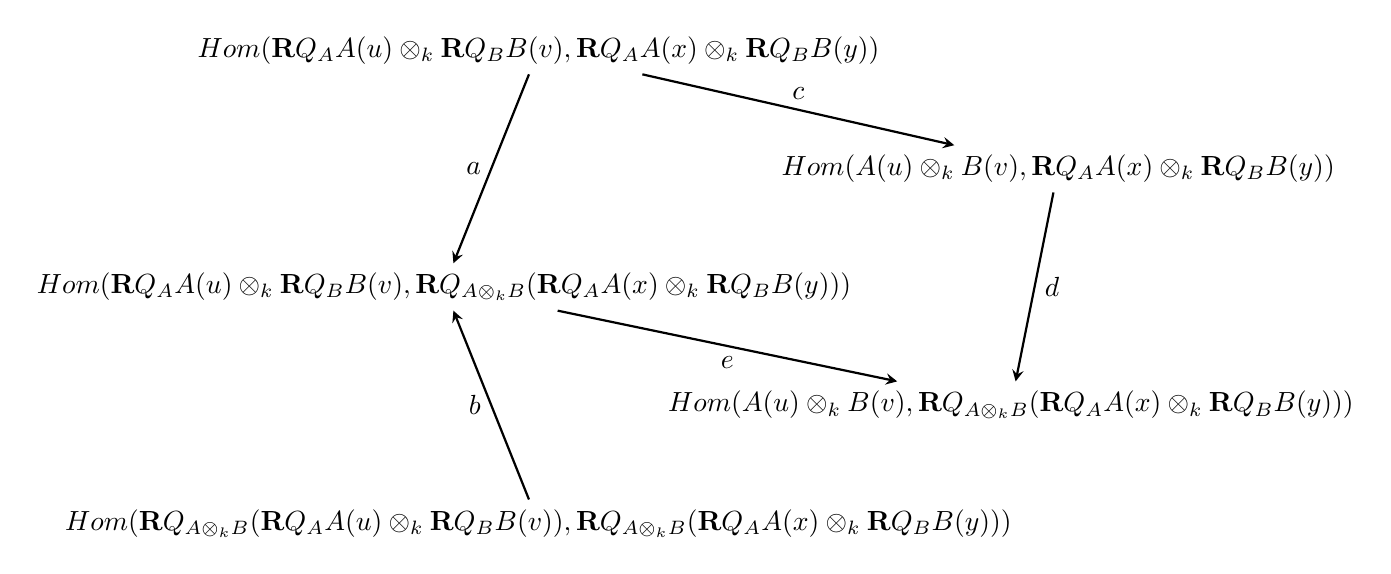
\begin{tikzpicture}[scale=.6,level/.style={->,>=stealth,thick}]
	\node (a) at (-5,5) {\(\op{Hom}(\mathbf{R} Q_A A(u) \otimes_k \mathbf{R} Q_B B(v),\mathbf{R} Q_A A(x) \otimes_k \mathbf{R} Q_B B(y))\)};
	\node (b) at (6,2.5) {\(\op{Hom}(A(u) \otimes_k B(v),\mathbf{R} Q_A A(x) \otimes_k \mathbf{R} Q_B B(y))\)};
	\node (c) at (-7,0) {\(\op{Hom}(\mathbf{R} Q_A A(u) \otimes_k \mathbf{R} Q_B B(v),\mathbf{R}Q_{A \otimes_k B} (\mathbf{R} Q_A A(x) \otimes_k \mathbf{R} Q_B B(y)))\)};
	\node (d) at (5,-2.5) {\(\op{Hom}(A(u) \otimes_k B(v),\mathbf{R}Q_{A \otimes_k B} (\mathbf{R} Q_A A(x) \otimes_k \mathbf{R} Q_B B(y)))\)};
	\node (e) at (-5,-5) {\(\op{Hom}(\mathbf{R}Q_{A \otimes_k B} (\mathbf{R} Q_A A(u) \otimes_k \mathbf{R} Q_B B(v)),\mathbf{R}Q_{A \otimes_k B} (\mathbf{R} Q_A A(x) \otimes_k \mathbf{R} Q_B B(y)))\)};
	\draw[level] (a) -- node[left] {\(a\)} (c) ;
	\draw[level] (e) -- node[left] {\(b\)} (c) ;
	\draw[level] (a) -- node[above] {\(c\)} (b) ;
	\draw[level] (b) -- node[right] {\(d\)} (d) ;
	\draw[level] (c) -- node[below] {\(e\)} (d) ;
    \end{tikzpicture} }
  \end{center}
  and we want to know first that \(a\) and \(b\) are quasi-isomorphisms. We know that \(b\) is a quasi-isomorphism since \(\mathbf{R}\tau_{A \otimes_k B}\) is left orthogonal to \(\mathbf{R}Q_{A \otimes_k B}\) so we only need to check \(a\). Since \(A(u) \otimes_k B(v)\) is free and 
  \begin{displaymath}
    \mathbf{R} Q_A A(u) \otimes_k \mathbf{R} Q_B B(v) \to \mathbf{R}Q_{A \otimes B} (\mathbf{R} Q_A A(u) \otimes_k \mathbf{R} Q_B B(v) )
  \end{displaymath}
  is a quasi-isomorphism, \(d\) is a quasi-isomorphism. Since \(\mathbf{R}Q_A\) and \(\mathbf{R}Q_B\) commute with coproducts, using tensor-Hom adjunction shows that \(c\) is a quasi-isomorphism. Finally, since the cone over the map
  \begin{displaymath}
    A(u) \otimes_k A(v) \to \mathbf{R} Q_A A(u) \otimes_k \mathbf{R} Q_B B(v)
  \end{displaymath}
  is annihilated by \(\tau_{A \otimes_k B}\), we see that \(e\) is also a quasi-isomorphism. This implies that \(a\) is a quasi-isomorphism.
  By an analogous argument, the endomorphisms of \(\mathbf{R}Q_{A \otimes B} (A(u) \otimes_k B(v))\) and \(\mathbf{R}Q_{A \otimes B} (\mathbf{R} Q_A A(u) \otimes_k \mathbf{R} Q_B B(v) )\) are quasi-isomorphic.
\end{proof}


\section{The quasi-equivalence}

Now we turn to the main result. 

\begin{theorem} \label{theorem: derived morita for NCP}
  Let \(k\) be a field. Let \(A\) and \(B\) be connected graded \(k\)-algebras. If \(A\) and \(B\) form a tasty pair, then there is a natural quasi-equivalence 
  \begin{displaymath}
    F : \hinj{\QGr{A^\opp \otimes_k B}} \to \RHomc{ \hinj{\QGr{A}}, \hinj{\QGr{B}} }
  \end{displaymath}
  such that for an object \(P\) of \(\mathrm{D}(\QGr{A^\opp \otimes_k B})\), the exact functor \(H^0(F(P))\) is isomorphic to 
  \begin{displaymath}
    \Phi_P(M) :=  \pi_B \left( \mathbf{R}\omega_{A^\opp \otimes_k B} P \overset{\mathbf{L}}{\otimes}_{\mathcal A} \mathbf{R}\omega_A M \right).
  \end{displaymath}
\end{theorem}

\begin{proof}
  Applying Corollary~\ref{corollary: Toen}, it suffices to provide a quasi-equivalence
  \begin{displaymath}
    G : \hinj{\QGr{A^\opp \otimes_k B}} \to \hproj{ (Q \mathcal A)^\opp \otimes_k Q \mathcal B}
  \end{displaymath}
  Using Corollary~\ref{corollary: duality is a duality}, we have a quasi-equivalence
  \begin{displaymath}
    \hproj{ (Q \mathcal A)^\opp \otimes_k Q \mathcal B} \cong \hproj{ Q \mathcal A^\opp \otimes_k Q \mathcal B}. 
  \end{displaymath}
  From Lemma~\ref{lemma: another model for QA otimes QB} we have a quasi-fully faithful functor 
  \begin{displaymath}
    Q \mathcal A^\opp \otimes_k Q \mathcal B \to \hinj{\QGr{A^\opp \otimes_k B}}. 
  \end{displaymath}
  This gives a functor 
  \begin{displaymath}
    \hinj{\QGr{A^\opp \otimes_k B}} \to \hproj{Q \mathcal A^\opp \otimes_k Q \mathcal B}
  \end{displaymath}
  which is a quasi-equivalence by a standard argument, see e.g. \parencite[Theorem 5.1]{Dyckerhoff11}.
  
  Tracing out the quasi-equivalences, one just needs to manipulate 
  \begin{align*}
    \op{Hom} (\mathbf{R}Q_A A(x)^\vee \otimes_k \mathbf{R}Q_B B(y), P) & \cong \op{Hom} ( \mathbf{R}Q_B B(y) , \op{Hom}( \mathbf{R}Q_A A(x)^\vee, \mathbf{R}\omega_{A^\opp \otimes_k B} P)) \\
    & \cong \op{Hom} ( \mathbf{R}Q_B B(y) , \mathbf{R}\omega_{A^\opp \otimes_k B} P \overset{\mathbf{L}}{\otimes}_{\mathcal A} \mathbf{R}Q_A A(x) ) 
  \end{align*}
  using Propostion~\ref{proposition: vanishing of tensor} and Lemma~\ref{lemma: trace map}. This says that the induced continuous functor is
  \begin{displaymath}
    M \mapsto \pi_B \left( \mathbf{R}\omega_{A^\opp \otimes_k B} P \overset{\mathbf{L}}{\otimes}_{\mathcal A} \mathbf{R}\omega_A M \right). 
  \end{displaymath}
\end{proof}

The following statement is now a simple application of Theorem~\ref{theorem: derived morita for NCP} and results of \parencite{Lunts-Orlov}. 

\begin{corollary} \label{corollary: NCP morita}
  Let \(A\) and \(B\) be a tasty pair of connected graded \(k\)-algebras with \(k\) a field. Assume that there exists an equivalence
  \begin{displaymath}
    f : \mathrm{D} (\QGr{A}) \to \mathrm{D} (\QGr{B}).
  \end{displaymath}
  Then there exists an object \(P \in D ( \QGr{A^\opp \otimes_k B} )\) such that 
  \begin{displaymath}
    \Phi_P : \mathrm{D} ( \QGr{A}) \to \mathrm{D} (\QGr{B} )
  \end{displaymath}
  is an equivalence.
\end{corollary}

\begin{proof}
  Applying \parencite[Theorem 1]{Lunts-Orlov} we know there is a quasi-equivalence between the unique enhancements, i.e. there is an \( F \in [ \hinj{ \QGr{A}}, \hinj{ \QGr{B}} ]\) giving an equivalence
  \begin{displaymath}
    H^0(F) : H^0(\hinj{ \QGr{A} }) = \mathrm{D}(\QGr{A}) \to H^0(\hinj{ \QGr{B} }) = \mathrm{D}(\QGr{B}).
  \end{displaymath}
  Then, by Theorem~\ref{theorem: derived morita for NCP}, there exists a \(P \in \mathrm{D}(\QGr{A^\opp \otimes_k B})\) such that \(\Phi_P = H^0(F)\). 
\end{proof}

%TODO: Determine if this gets yanked into Section 2 or not.
We wish to identify the kernels as objects of the derived category of an honest noncommutative projective scheme.  Towards this end, we define a graded ring associated to a pair of graded \(k\)-algebras.
\begin{definition}\label{def: segre product}
  Let \(A\) and \(B\) be connected graded \(k\)-algebras.
  The \textbf{Segre product} of \(A\) and \(B\) is the graded \(k\)-algebra
  \[ A \times_k B = \bigoplus_{0 \leq i} A_i \otimes_k B_i.\]
\end{definition}

In general, one can only hope that kernels obtained as above are objects of the derived category of a noncommutative (bi)projective scheme.
However, we have the following special case in which we can collapse the \(\Z^2\)-grading to a \(\Z\)-grading.
Denote by \(\A \times \B\) the dg-category with objects \(\Z\) and morphisms \(\A \times \B(i,j)\) the chain complex with \(A_i \otimes_k B_i\) in degree zero.

\begin{lemma}\label{lemma: Q(AxB) is Q(A tensor B)}
  Assume \(A\) and \(B\) satisfy (insert hypotheses here).
  Then there is a quasi-equivalence
  \[Q(\A \times \B) \to Q(\A \otimes \B)\]
\end{lemma}

\begin{proof}
  We have an obvious functor \(\Delta \colon \A \times \B \to \A \otimes \B\) defined by \(\Delta(i) = (i,i)\) on objects with structure morphism the identity.
  %\[ \A \times \B(i,j) = A_{j-i} \otimes_k B_{j-i} \to A_{j-i} \otimes_k B_{j-i}= \A \otimes \B((i,i), (j,j)).\]
  This yields an adjoint pair of dg-functors \(\Ind{\Delta} \colon \dgMod{\A \times \B} \to \dgMod{\A \otimes \B}\) and \(\Res{\Delta} \colon \dgMod{\A \otimes \B} \to \dgMod{\A \times \B}\).
  Moreover, it is easy to check that \(\Ind{\Delta}\) is induced by the object \(P\) of \(\dgMod{\left(\A \times \B\right)^\opp \otimes \left(\A \otimes \B \right)}\) defined by
  \[P(i,(m,n)) = \left(\A \otimes \B\right)^\opp\left((i,i),(m,n)\right) = A_{i- m} \otimes_k B_{i - n}\]
  in the sense that \(\Ind{\Delta} \cong \widehat{\Phi_P} = - \otimes_{\A \times \B} P\).
\end{proof}
\begin{corollary} \label{corollary: NCP morita degree 1}
  Let \(A\) and \(B\) be a tasty pair of connected graded \(k\)-algebras with \(k\) a field that are both generated in degree one.
  Assume that there exists an equivalence
  \begin{displaymath}
    f : \mathrm{D} (\QGr{A}) \to \mathrm{D} (\QGr{B}).
  \end{displaymath}
  Then there exists an object \(P \in D ( \QGr{A^\opp \times_k B} )\) such that 
  \begin{displaymath}
    \Phi_P : \mathrm{D} ( \QGr{A}) \to \mathrm{D} (\QGr{B} )
  \end{displaymath}
  is an equivalence.
\end{corollary}

\begin{proof}
\end{proof}

%\chapter{Background}

\documentclass[dissertation.tex]{subfiles}
\begin{document}
\section{Differential Graded Modules and Algebras}
{\noindent Throughout, let $k$ be a commutative ring.}

\begin{defn}
  A {\it differential graded $k$-module}, $M$, is a complex of $k$-modules
  $$M \colon \begin{tikzcd}
    \cdots \arrow{r}{d_M^{n-2}} & M^{n-1} \arrow{r}{d_M^{n-1}} & M^n \arrow{r}{d_M^n} & M^{n+1} \arrow{r}{d_M^{n+1}} & \cdots
  \end{tikzcd},$$
  or, equivalently, a $\Z$-graded module over the graded ring $k$, concentrated in degree 0, equipped with a degree one morphism $d_M : M \rightarrow M[1]$ such that $d_M^2 = 0$.
  A {\it morphism of differential graded $k$-modules} is a morphism of chain complexes.
  
  The {\it shift} of a dg $k$-module is the shifted complex
  $$M[1] \colon \begin{tikzcd}
    \cdots \arrow{r}{-d_M^{n-1}} & M^{n} \arrow{r}{-d_M^{n}} & M^{n+1} \arrow{r}{-d_M^{n+1}} & M^{n+2} \arrow{r}{-d_M^{n+2}} & \cdots
  \end{tikzcd}$$
  
  The tensor product of two dg $k$-modules is the usual tensor product in $\Ch{k}$, the category of chain complexes of $k$-modules.
\end{defn}

\begin{defn}
  We say a category, $\CC$, is a {\it $k$-category} if
  \begin{enumerate}
  \item
    for each pair of objects $X$ and $Y$ of $\CC$, $\Hom{\CC}{X,Y}$ is a $k$-module, and
  \item
    composition 
    $$\Hom{\CC}{X,Y} \otimes_k \Hom{\CC}{Y,Z} \rightarrow \Hom{\CC}{X,Z}$$
    in $\CC$ is $k$-linear, associative, admitting units $\id_X \in \Hom{\CC}{X,X}$.
  \end{enumerate}
\end{defn}

\section{The Category of Differential Graded Categories}

\begin{defn}
  A {\it differential graded} or {\it dg category} is a $k$-category, $\CC$, satisfying
  \begin{enumerate}
  \item
    $\Hom{\CC}{X,Y}$ is a dg $k$-module for all objects $X,Y$ of $\CC$, and
  \item
    composition 
    $$\begin{tikzcd}
      \Hom{\CC}{X,Y} \otimes_k \Hom{\CC}{Y,Z} \arrow{r} & \Hom{\CC}{X,Z}
    \end{tikzcd}$$
    in $\CC$ is a morphism of dg $k$-modules;
    that is a morphism of $\Ch{k}$.
  \end{enumerate}
  
  A {\it morphism of dg categories}, or {\it dg functor}, $\mathscr{F} \colon \CC \rightarrow \D$, is a functor such that
  $$F(X,Y) \colon 
  \begin{tikzcd}
    \Hom{\CC}{X,Y} \arrow{r} & \Hom{\D}{FX,FY}
  \end{tikzcd}$$
  is a morphism of dg $k$-modules.
  Denote by $\operatorname{dgcat}_k$ the category with objects small dg categories and morphisms dg functors.
\end{defn}

\begin{eg}
  \begin{description}[style=nextline]
  \item[dg category with one object]
    Let $A$ be a dg $k$-algebra; that is, a graded $k$-algebra equipped with a differential
    $$d(fg) = d(f)g + (-1)^nfd(g),\ f \in A^n, g \in A.$$
    Define $\mathscr{A}$ to be the category with one object, $\ast$, and morphisms $\mathscr{A}(\ast, \ast) = A$, with composition defined by the multiplication in $A$.
  \item[dg $k$-modules]
    Define the category $\mathcal{C}_\text{dg}(k)$ to have objects chain complexes of $k$-modules, and morphisms $\mathcal{C}_\text{dg}(k)(C,D) = [C,D]_{\Ch{k}}$, the internal hom for $\Ch{k}$ as in Definition~\ref{ChInternalHomDefn}.
    The composition of morphisms
    $$\begin{tikzcd}
      \cdg{k}(C,D) \otimes_k \cdg{k}(D,E) \arrow{r} & \cdg{k}(C,E)
    \end{tikzcd}$$
    is the composition morphism of Remark~\ref{MorphismsOfDGModules} (\ref{MorphismsOfDGModules.composition}).
    
    As an immediate consequence of Proposition~\ref{ChHomTensorAdjunction} we have the following observation:
    \begin{prop}
      %The category $\mathcal{C}_\text{dg}(k)$ is both a tensored and cotensored $\Ch{k}$-category.
      For any three chain complexes, $C$, $D$, and $E$, there is a canonical isomorphism of chain complexes
      $$\cdg{k}(C \otimes_k E, D) \cong \cdg{k}(C,\cdg{k}(E,D)).$$
      
      \begin{proof}
        Let $X$ be any object of $\Ch{k}$.
        Using the adjunction of Proposition~\ref{ChHomTensorAdjunction} we have
        \begin{eqnarray*}
          \Ch{k}(X,\cdg{k}(C \otimes_k E, D) &\cong& 
          \Ch{k}(X \otimes_k (C \otimes_k E), D)\\
          &\cong& \Ch{k}((X \otimes_k C) \otimes_k E, D)\\
          &\cong& \Ch{k}(X \otimes_k C, \cdg{k}(E,D))\\
          &\cong& \Ch{k}(X, \cdg{k}(C, \cdg{k}(E,D)).
        \end{eqnarray*}
        Therefore by the Yoneda Lemma there is a unique isomorphism 
        $$\cdg{k}(C \otimes_k E, D) \cong \cdg{k}(C, \cdg{k}(E,D)).$$
      \end{proof}
    \end{prop}
    %Note that $[C,D]$ is, equivalently, the graded module of graded morphisms; that is, a morphism $f \in \mathcal{C}_\text{dg}(k)(C, D)^m$ is a collection of morphisms $f^n \colon C^n \rightarrow D^{n+m}$.
    %Equip $\mathcal{C}_\text{dg}(k)(C, D)$ with the differential
    %$$\begin{tikzcd}
    %  \mathcal{C}_\text{dg}(k)(C, D)^n \arrow{r} & \mathcal{C}_\text{dg}(k)(C, D)^{n+1}\\
    %  f \arrow[mapsto]{r} & d_D \circ f + (-1)^{n+1}f \circ d_C
    %\end{tikzcd}$$
    %and define composition of morphisms by the tensor product in $\mathcal{C}(k)$,
    %$$\begin{tikzcd}
    %  \mathcal{C}_\text{dg}(k)(D, E) \otimes_k \mathcal{C}_\text{dg}(k)(C, D) \arrow{r} & \mathcal{C}_\text{dg}(k)(C, E).
    %\end{tikzcd}$$
  \end{description}
\end{eg}

\begin{defn}
  Let $\CC$ and $\D$ be objects of $\operatorname{dgcat}_k$.
  The {\it tensor product}, $\CC \otimes \D$, is the dg category with objects $\operatorname{ob}\CC \times \operatorname{ob}\D$ and
  morphisms
  $$\begin{tikzcd}
    \Hom{\CC \otimes \D}{(X, Y), (X^\prime, Y^\prime)} = \Hom{\CC}{X,X^\prime} \otimes_k \Hom{\D}{Y,Y^\prime}.
  \end{tikzcd}$$
  For ease of notation, we will denote by $X \otimes Y$ the object $(X,Y)$ of $\CC \otimes \D$.
\end{defn}

\begin{defn}
  Given two dg functors $\mathscr{F},\mathscr{G} \colon \CC \rightarrow \D$, define $\SHom{\mathscr{F},\mathscr{G}}^n$ to be the $k$-module of degree $n$ natural transformations.
  That is, morphisms of functors, $\eta \colon \mathscr{F} \rightarrow \mathscr{G}$ such that for each object $X$ of $\CC$, $\eta(X) \in \Hom{\D}{\mathscr{F}(X),\mathscr{G}(X)}^n$.
\end{defn}

\begin{prop}
  Given a degree $n$ natural transformation $\eta \colon \mathscr{F} \rightarrow \mathscr{G}$, the collection of morphisms
  $$d^n_{\Hom{\D}{\mathscr{F}X, \mathscr{G}X}}\left( \eta(X) \right) \in \Hom{\D}{\mathscr{F}X, \mathscr{G}X}^{n+1}$$
  define a natural transformation of degree $n + 1$ and hence endow $\SHom{\mathscr{F},\mathscr{G}}$ with the structure of a dg $k$-module, where the differential, $d_{\SHom{\mathscr{F},\mathscr{G}}}^n$ sends $\eta$ to this natural transformation.
  
  \begin{proof}
    It's clear that so long as the collection of $d^n_{\D(\F X, \G X)}(\eta(X))$ defines a natural transformation, the resulting sequence
    $$\begin{tikzcd}
      \cdots \arrow{r} & \SHom{\F, \G}^n \arrow{r} & \SHom{\F,\G}^{n+1} \arrow{r} & \cdots
    \end{tikzcd}$$
    will be a complex.
    
    First we note that, by definition, any dg functor necessarily commutes with the differentials:
    $$d_{\D(\mathscr{F}X, \mathscr{F}X^\prime)}\left(\mathscr{F}(f) \right) = \mathscr{F}\left(d_{\CC(X,X^\prime)}(f)\right)$$
    and composition is a morphism of dg $k$-modules, so we have the commutative diagrams
    $$\begin{tikzcd}
      \D(\F X^\prime, \G X^\prime) \otimes_k \D(\F X, \F X^\prime) \arrow{r}\arrow[swap]{d}{d \otimes 1 + 1 \otimes d}& \D(\F X, \G X^\prime)\arrow{d}{d}\\
      \D(\F X^\prime, \G X^\prime) \otimes_k \D(\F X, \F X^\prime)[1] \arrow{r}& \D(\F X, \G X^\prime)[1]
    \end{tikzcd}$$
    and
    $$\begin{tikzcd}
      \D(\G X, \G X^\prime) \otimes_k \D(\F X, \G X) \arrow{r}\arrow[swap]{d}{d \otimes 1 + 1 \otimes d}& \D(\F X, \G X^\prime)\arrow{d}{d}\\
      \D(\G X, \G X^\prime) \otimes_k \D(\F X, \G X)[1] \arrow{r}& \D(\F X, \G X^\prime)[1]
    \end{tikzcd}$$
    For a morphism $f \in \CC(X,X^\prime)$, chasing $\eta(X^\prime) \otimes \F(f)$ and $\G(f) \otimes \eta(X)$ through the diagram gives
    \begin{eqnarray*}
      d(\eta(X^\prime)) \circ \F(f) + \eta(X^\prime) \circ d(\F(f)) 
      &=& d(\eta(X^\prime) \circ \F(f))\\
      &=& d(\G(f) \circ \eta(X))\\
      &=& d(\G(f)) \circ \eta(X) + \G(f) \circ d(\eta(X)).
    \end{eqnarray*}
    By the fact that $\F$,$\G$ commute with differentials and $\eta$ is a natural tranformation, we see
    $$\eta(X^\prime) \circ d(\F(f)) = \eta(X^\prime) \circ \F(d(f)) = \G(d(f)) \circ \eta(X) = d(\G(f)) \circ \eta(X).$$
    Therefore
    $$d(\eta(X^\prime)) \circ \F(f) = \G(f) \circ d(\eta(X)),$$
    as desired.
  \end{proof}
\end{prop}

\begin{defn}
  For two objects $\CC$ and $\D$ of $\operatorname{dgcat}_k$, define the object $\SHom{\CC,\D}$ of $\operatorname{dgcat}_k$ to be the category with objects dg functors $\mathscr{F} \colon \CC \rightarrow \D$ and morphisms $\SHom{\mathscr{F},\mathscr{G}}$.
  
  Given two dg functors $\F,\G \colon \CC \rightarrow \D$, define a {\it morphism of dg functors}, $\eta \colon \F \rightarrow \G$ to be a closed, degree zero natural transformation.
  That is, $\eta \in \SHom{\F, \G}^0$ and its image in $\SHom{\F,\G}^1$ under the differential is zero.
\end{defn}

\begin{rmk}
  There is a natural isomorphism of bifunctors
  $$\Hom{\operatorname{dgcat}_k}{\CC \otimes \D, \mathscr{E}} \cong \Hom{\operatorname{dgcat}_k}{\CC, \SHom{\D,\mathscr{E}}},$$
  which endows $\operatorname{dgcat}_k$ with a symmetric closed monoidal structure.
\end{rmk}

\begin{defn}
  Let $\CC$ be a dg category.
  Define
  \begin{enumerate}
  \item
    the category $Z^0(\CC)$ to be the category with objects those of $\CC$ and morphisms
    $$\Hom{Z^0(\CC)}{X,Y} = Z^0\left(\Hom{\CC}{X,Y}\right),$$
  \item
    the category $H^0(\CC)$ to be the category with objects those of $\CC$ and morphisms
    $$\Hom{H^0(\CC)}{X,Y} = H^0\left(\Hom{\CC}{X,Y}\right),$$
  \item
    the {\it homology category}, $H^\ast(\CC)$, to be the category with objects those of $\CC$ and morphisms 
    $$H^\ast\CC(X,Y) = \bigoplus H^n\CC(X,Y).$$
  \end{enumerate}
\end{defn}

\begin{rmk}\label{DGInducedHomology}
  Note that given a dg functor, $\mathscr{F} \colon \CC \rightarrow \D$, for $X$ and $Y$ objects of $\CC$, 
  $$\mathscr{F}(X,Y) \colon \CC(X,Y) \rightarrow \D(\mathscr{F}X, \mathscr{F}Y)$$
  is a morphism of $\mathcal{C}(k)$ and this immediately implies the diagram
  $$\begin{tikzcd}
    B^n(\CC(X,Y))\arrow{r}{\imath^n}\arrow[bend left]{rr}{\im d^{n-1}}\arrow[dashed]{d}{\exists !B^n(\F(X,Y))} & Z^n(\CC(X,Y)) \arrow{r}{\ker d^n}\arrow[dashed]{d}{\exists !Z^n(\F(X,Y))} & \CC(X,Y)^{n} \arrow{d}{\F(X,Y)}\\
    B^n(\D(\F X,\F Y) \arrow{r}{\imath^n}\arrow[bend right]{rr}{\im d^{n-1}} & Z^n(\D(\F X,\F Y))\arrow{r}{\ker d^n} & \D(\F X,\F Y)^{n}
  \end{tikzcd}$$
  commutes for each $n$.
  Hence $H^n$ induces a functor
  $H^n(\mathscr{F}) \colon H^n(\CC) \rightarrow H^n(\D)$
  with object map\\ $H^n(\mathscr{F})(X) = \mathscr{F}(X)$ and induced arrow map 
  $$\begin{tikzcd}
    0 \arrow{r} & B^n(\CC(X,Y))\arrow{r}{\imath^n}\arrow{d}{B^n(\F(X,Y))} & Z^n(\CC(X,Y)) \arrow{r}{\coker \imath^n}\arrow{d}{Z^n(\F(X,Y))} & H^n(\CC(X,Y)) \arrow[dashed]{d}{\exists !H^n(\F(X,Y))}\arrow{r} & 0 \\
    0 \arrow{r} & B^n(\D(\F X,\F Y) \arrow{r}{\imath^n} & Z^n(\D(\F X,\F Y))\arrow{r}{\coker \imath^n} & H^n(\D(\F X,\F Y)) \arrow{r} & 0
  \end{tikzcd}$$
\end{rmk}

\section{Modules over a Differential Graded Category}

\begin{defn}
  Let $\CC$ be a small dg category and let $\mathscr{M} : \CC \rightarrow \mathcal{C}_\text{dg}(k)$ be a dg functor.
  \begin{enumerate}
  \item
    We say that $\mathscr{M}$ is a right (resp. left) dg $\CC$-module if $\mathscr{M}$ is contravariant (resp. covariant).
  \item
    The {\it homology of a dg $\CC$-module}, $\mathscr{M}$, is the induced functor
    $$\begin{tikzcd}
      H^\ast(\CC) \arrow{r}{H^\ast(\mathscr{M})}& \Gr{k}\\
      X \arrow[mapsto]{r} & H^\ast(\mathscr{M}(X))
      %H^\ast(\CC(Y,X)) \arrow[mapsto]{r} & H^\ast(\mathcal{C}_\text{dg}(\mathscr{M}(X),\mathscr{M}(Y))
    \end{tikzcd}$$
    where $\Gr{k}$ denotes the category of graded modules.
  \item
    Define the category of dg $\CC$-modules $\mathcal{C}_\text{dg}(\CC) = \SHom{\CC, \mathcal{C}_\text{dg}(k)}$, and the category of right $\CC$-modules by
    $$\mathcal{C}(\CC) = Z^0 \mathcal{C}_\text{dg}(\CC).$$
    Note that the morphisms of this category are just $\Ch{k}$-natural transformations and this endows $\mathcal{C}(\CC)$ with the structure of an abelian category.
    %TODO: This should probably be justified at some point; either in here, or somewhere else.  It's not immediately clear at the moment.
    \item
      A morphism $\eta \colon \mathscr{L} \rightarrow \mathscr{M}$ of $\CC$-modules is the data of a collection of morphisms $\eta(X) \in \Ch{k}(\funct{L}X,\funct{M}X)$, natural in $X$.
      As such, each $\eta(X)$ induces a morphism
      $$H^\ast(\eta(X)) \colon H^\ast(\funct{L}X) \to H^\ast(\funct{M}X)$$
      and naturality of $\eta$ ensures naturality of $H^\ast(\eta)$, giving a morphism
      $$H^\ast(\eta) \colon H^\ast(\mathscr{L}) \rightarrow H^\ast(\mathscr{M}).$$
      We say $\eta$ is a {\it quasi-isomorphism} if $H^\ast(\eta)$ is an isomorphism.
  \end{enumerate}
\end{defn}

\subsection{The Category up to Homotopy}
\begin{defn}
    Let $\CC$ be a small dg category.
    The {\it category up to homotopy of dg $\CC$-modules} is defined to be $\mathcal{H}(\CC) = H^0(\mathcal{C}_\text{dg}(\CC))$.
    %Note that $\mathcal{H}(\CC)$ is a triangulated category.
    %TODO: Is this obviously just the same proof for K(A), where A is an abelian category?
\end{defn}

Given a dg $\CC$-module, $\mathscr{M} \colon \CC^\text{op} \rightarrow \mathcal{C}_\text{dg}(k)$, by Remark~\ref{DGInducedHomology} we have a well-defined map
$$Z^0(\mathscr{M}(Y,X)) \colon
\begin{tikzcd}
  Z^0(\CC(Y,X)) \arrow{r} & Z^0(\mathcal{C}_\text{dg}(k)(\mathscr{M}X,\mathscr{M}Y)) = \mathcal{C}(k)(X,Y)
\end{tikzcd}$$
which allows us to view the image of $\mathscr{M}$ in $\mathcal{C}(\CC)$ as a presheaf $\mathscr{M} \colon Z^0(\CC) \to \mathcal{C}(k)$.

\begin{defn}
  Given a morphism $\eta \in \mathcal{C}(\CC)(\mathscr{L}, \mathscr{M})$, we note that for each object $X$ of $\CC$, $\eta(X)$ is a morphism of chain complexes.
  Define the dg functor $\cone{\eta} \colon \CC^\text{op} \rightarrow \mathcal{C}_\text{dg}(k)$ as follows.
  For each object $X$ of $\CC$ we have the chain complex $\cone{\eta}(X) = \cone{\eta(X)}$ equipped with the differential
  $$d_{\cone{\eta}(X)} = \left(\begin{matrix}
    d_{\mathscr{L}(X)[1]} & 0\\
    \\
    -\eta(X)[1] & d_{\mathscr{M}(X)}
  \end{matrix}\right).$$

  Given a morphism $f \in \CC(Y,X)^n$, we define $\cone{\eta}(f)$ by
  $$\begin{tikzcd}[ampersand replacement=\&]
      \cone{\eta}(X) \arrow{rrrr}{\left(\begin{matrix}(-1)^n\mathscr{L}(f)[1] & 0\\0 & \mathscr{M}(f)\end{matrix}\right)} \&\&\&\& \cone{\eta}(Y)[n]
    \end{tikzcd}.$$
  Since both $\mathscr{L}$ and $\mathscr{M}$ are dg functors and $\eta$ is natural, it is straightforward to see that this gives a morphism of complexes
  $$\begin{tikzcd}
    \CC(Y,X) \arrow{r} & \mathcal{C}(k)(\cone{\eta(X)}, \cone{\eta(Y)})
  \end{tikzcd}$$
\end{defn}

\begin{rmk}
  \begin{enumerate}
  \item
    Note that if we are given a morphism $f \in Z^0(\CC(Y,X))$, then $\mathscr{L}(f)$ and $\mathscr{M}(f)$ are both morphisms of complexes and $\eta$ is natural, so we obtain a morphism of complexes, $\cone{\eta}(f)$,
    $$\begin{tikzcd}[ampersand replacement=\&]
      \cone{\eta}(X) \arrow{rrr}{\left(\begin{matrix}\mathscr{L}(f)[1] & 0\\0 & \mathscr{M}(f)\end{matrix}\right)} \&\&\& \cone{\eta}(Y)
    \end{tikzcd}.$$
  \item
    We also note that we have a short exact sequence of $\CC$-modules
    $$\begin{tikzcd}
      0 \arrow{r} & \mathscr{M} \arrow{r}{\left(\begin{matrix}0\\1\end{matrix}\right)} & \cone{\eta} \arrow{r}{\left(-1\ 0\right)} & \mathscr{L}[1] \arrow{r} & 0
    \end{tikzcd}$$
  \end{enumerate}
\end{rmk}

\begin{prop}
  The category $\mathcal{H}(\CC)$ with distinguished triangles those triangles that are isomorphic to the image of
  $$\begin{tikzcd}
    \mathscr{L} \arrow{r}{\eta} & \mathscr{M} \arrow{r} & \cone{\eta} \arrow{r} & \mathscr{L}[1] 
  \end{tikzcd}$$
  in $\mathcal{H}(\CC)$ is triangulated.

  \begin{proof}
    First, suppose that we are given two morphisms $\eta, \nu \in \mathcal{C}(\CC)(\mathscr{L},\mathscr{M})$ having the same image in $\mathcal{H}(\CC)(\mathscr{L},\mathscr{M})$.
    By definition, there exists a morphism $h \in \mathcal{C}_\text{dg}(\CC)(\mathscr{L},\mathscr{M})^{-1}$ such that 
    $$\eta - \nu = d_{\mathcal{C}_\text{dg}(\CC)(\mathscr{L},\mathscr{M})}^{-1}(h) = d_\mathscr{M} \circ h + h \circ d_\mathscr{L}.$$
    It's straightforward to show that
    $$\begin{tikzcd}[ampersand replacement=\&]
      \cone{\eta} \arrow{r}{\left(\begin{matrix}1 & 0\\-h & 1\end{matrix}\right)} \& \cone{\nu}
    \end{tikzcd}
    \ \text{and}\ 
    \begin{tikzcd}[ampersand replacement=\&]
      \cone{\nu} \arrow{r}{\left(\begin{matrix}1 & 0\\h & 1\end{matrix}\right)} \& \cone{\eta}
    \end{tikzcd}$$
    give mutually inverse morphisms of $\mathcal{C}(\CC)$, so the triangles are well-defined.
    
    For (TR1) we see that given any morphism $\overline{\eta} \in \mathcal{H}(\CC)(\mathscr{L},\mathscr{M})$, we can fit $\overline{\eta}$ into a distinguished triangle by lifting to $\mathcal{C}(\CC)$ and taking the image of
    $$\begin{tikzcd}
      \mathscr{L} \arrow{r}{\eta} & \mathscr{M} \arrow{r} & \cone{\eta} \arrow{r} & \mathscr{L}[1]
    \end{tikzcd}$$
    in $\mathcal{H}(\CC)$.
  \end{proof}
\end{prop}
\section{The Model Structure on $\mathcal{C}(\CC)$}


\begin{defn}[\cite{Toen}]
  Let $\CC$ be a small dg category and $\eta \colon \funct{L} \to \funct{M}$ a morphism of $\mathcal{C}(\CC)$.
  Equipping $\Ch{K}$ with the projective model structure, we say the morphism $\eta$ is a weak-equivalence (resp. fibration) if for each object $X$ of $\CC$ the morphism
  $$\eta(X) \in \Ch{k}(\funct{L}X, \funct{M}X)$$
  is a weak-equivalence (resp. fibration).
  This endows $\mathcal{C}(\CC)$ with the structure of a cofibrantly generated model category in the sense of \cite{HoveyMC}, 2.1.
  %From Keller
  %A dg $\CC$-module, $\mathscr{M}$, is {\it cofibrant} if for every epimorphic quasi-isomorphism $\mathscr{L} \rightarrow \mathscr{N}$, every morphism $\mathscr{M} \rightarrow \mathscr{L}$ factors through $\mathscr{L}$,
  %$$\begin{tikzcd}
  %  & \mathscr{M}\arrow{d}\arrow[dashed,swap]{ld}{\exists}\\
  %  \mathscr{L} \arrow{r} & \mathscr{N} \arrow{r} & 0
  %\end{tikzcd}$$
\end{defn}

\begin{rmk}
  \ \\
  \begin{itemize}
  \item
  We note that the representables are all cofibrant by the Yoneda Lemma.
  Namely, given an object $X$ of $\CC$, a trivial cofibration (i.e. a level-wise epimorphic quasi-isomorphism) 
  $\eta \in \mathcal{C}(\CC)(\funct{L},\funct{M})$,
  and a morphism 
  $\nu \in \mathcal{C}(\CC)(h_X, \funct{M})$$ \cong \funct{M}(X)$ 
  we can pull the image of $\nu$ back along $\eta(X)$ to some\\
  $\xi \in \mathcal{C}(\CC)(h_X, \funct{L}) \cong \funct{L}(X),$
  giving the desired lift
  $$\begin{tikzcd}
    0 \arrow{r}\arrow{d} & \funct{L}\arrow{d}{\eta}\\
    h_X \arrow{r}{\nu}\arrow[dashed]{ur}{\exists \xi} & \funct{M}
  \end{tikzcd}$$
\item
  Regarding $\dgcat_k$ as the 2-category of $\Ch{k}$-enriched categories, it's clear from Proposition~\ref{modulesaretensored} that $\cdg{\CC}$ is a tensored and cotensored category, which gives rise to bifunctors
  $$\otimes: \cdg{k} \times \cdg{\CC} \to \cdg{\CC}\ \text{and}\ \cdg{k}(-,-) \colon \cdg{k}^\text{op} \times \cdg{\CC} \to \cdg{\CC}$$
  and isomorphisms 
  $$\cdg{k}(C, \cdg{\CC}(\F, \G)) 
  \cong \cdg{\CC}(C \otimes \F, \G)
  \cong \cdg{\CC}(\F, \cdg{k}(C,\G)).$$
  for each object $C$ of $\cdg{k}$, $\Ch{k}$-natural in $\F$ and $\G$.
  This is an adjunction of two variables in the sense of \cite{HoveyMC} 4.1.12 and the bifunctor endows $\cdg{\CC}$ with the structure of a $\Ch{k}$-module in the sense of \cite{HoveyMC}, 4.2.18.
  Applying $Z^0$ gives rise to an adjunction of two variables
  $$\mathcal{C}(k)(C, \cdg{\CC}(\F,\G))
  \cong \mathcal{C}(\CC)(C \otimes \F, \G)
  \cong \mathcal{C}(\CC)(\F, \cdg{k}(C,\G)).$$
  We show that this endows $\mathcal{C}(\CC)$ with a $\mathcal{C}(k)$-model structure.
  
  Since $\mathcal{C}(k)$ is a symmetric monoidal model category (see \cite{HoveyMC}, 4.2.13) with cofibrant unit $k$, the chain complex consisting of $k$ in degree zero, it suffices to show that the adjunction is Quillen.
  Given cofibrations $f \colon C \to D$ of $\mathcal{C}(k)$ and $\eta \colon \F \to \G$ of $\mathcal{C}(\CC)$,
  we have the pushout in $\mathcal{C}(\CC)$
  $$\begin{tikzcd}
    C \otimes \F \arrow{rr}{1 \otimes \eta}\arrow{dd}{f \otimes 1} && C \otimes \G \arrow{dd}{u_1}\arrow[bend left]{rdddd}{f \otimes 1}\\
    \\
    D \otimes \F \arrow{rr}{u_2}\arrow[bend right]{rrrdd}{1 \otimes \eta} && D \otimes \F \coprod_{C \otimes \F} C \otimes \G\arrow[dashed]{rdd}{\exists !f \square \eta}\\
    \\
    & & & D \otimes \G
  \end{tikzcd}$$
  and we must show that $f \square \eta$ is a cofibration that is trivial whenever either one of $f$ and $\eta$ is.
  Since $f \square \eta$ is just the data of morphisms $f \square \eta(X)$
%  $$\begin{tikzcd}
%    C \otimes \F(X) \arrow{rr}{1 \otimes \eta(X)}\arrow{dd}{f \otimes 1} && C \otimes \G(X) \arrow{dd}{u_1(X)}\arrow[bend left]{rdddd}{f \otimes 1}\\
%    \\
%    D \otimes \F(X) \arrow{rr}{u_2(X)}\arrow[bend right]{rrrdd}{1 \otimes \eta(X)} && D \otimes \F(X) \coprod_{C \otimes \F(X)} C \otimes \G(X)\arrow[dashed]{rdd}{\exists !(f \square \eta)(X)}\\
%    \\
%    & & & D \otimes \G(X)
%  \end{tikzcd}$$
  indexed by the objects of $\CC$, we reduce to the case that $(f \square \eta)(X)$ is a cofibration that is trivial provided either one $\eta(X)$ or $f$ is.
  By definition of the model structure on $\mathcal{C}(\CC$, $\eta(X)$ is a cofibration, so this follows directly from the fact that $\mathcal{C}(k)$ is a symmetric monoidal model category.
  We note that by \cite{HoveyMC} 4.3.1 this induces a Quillen adjunction 
  $$[C,\mathbb{R}\Hom{\cdg{\CC}}{\F,\G}]_{\mathcal{C}(k)}
  \cong [C \otimes^\mathbb{L} \F, \G]_{\mathcal{C}(\CC)}
  \cong [\F, \mathbb{R}\Hom{\cdg{k}}{C,\G}]_{\mathcal{C}(\CC)},$$
  where $[-,-]$ denotes morphisms of the homotopy category, $\mathbb{R}\operatorname{Hom}$ and $\otimes^\mathbb{L}$ are the right and left derived functors, respectively.
  \end{itemize}
\end{rmk}

%From Keller
%\begin{thm}
%  The category $\mathcal{C}(\CC)$ admits a projective model structure with weak equivalences quasi-isomorphisms and fibrations epimorphisms.
%  For this structure, each object is fibrant and the cofibrant objects are the cofibrant dg $\CC$-modules.
%\end{thm}

\section{The Derived Category of a Differential Graded Category}

\begin{defn}
  Let $\CC$ be a small dg category.
  The derived category $\mathcal{D}(\CC)$ is the localization of $\mathcal{C}(\CC)$ at the class of quasi-isomorphisms, $\operatorname{Ho}(\mathcal{C}(\CC))$.
  Equivalently, this is the Verdier quotient of $\mathcal{H}(\CC)$ by acyclics.
\end{defn}

\section{Generators of Differential Graded Categories}
\subsection{Pretriangulated Differential Graded Categories}

\begin{defn}
  Let $\CC$ be a small dg category.
  We have the Yoneda embedding 
  $$\begin{tikzcd}
    Z^0(\CC) \arrow{r}{h_{\_}} & \mathcal{C}(\CC)\\
    X \arrow[mapsto]{r} & h_X.
  \end{tikzcd}$$
  We say that $\mathscr{M} \colon \CC^\text{op} \rightarrow \mathcal{C}_\text{dg}(k)$ is {\it quasi-representable} if there is an object $X$ of $\CC$ such that $h_X$ is quasi-isomorphic to $\mathscr{M}$
  
  We say that $\CC$ is {\it pretriangulated} if
  \begin{enumerate}
  \item
    for each $n \in \Z$ and each object $X$ of $\CC$, $h_X[n]$ is quasi-representable, and
  \item
    for all $f \in Z^0(\CC)(X,Y)$, $\operatorname{cone}(f_*)$ is quasi-representable, where $f_* : h_X \rightarrow h_Y$ is the image of $f$ under the Yoneda embedding.
  \end{enumerate}
\end{defn}

\begin{defn}
  Let $\CC$ be a pretriangulated dg category and let $E$ be an object of $\CC$.
  By abuse of notation, 
  \begin{enumerate}
  \item
    We say $E$ is a {\it classical generator} of $\CC$ if $h_E$ is a classical generator of $H^0(\CC)$,
  \item
    We say $E$ is a {\it strong generator} of $\CC$ if $h_E$ is a strong generator of $H^0(\CC)$,
  \item
    We say $E$ is a {\it (weak) generator} of $\CC$ if $h_E$ is a (weak) generator of $H^0(\CC)$, and
  \item
    We say $\CC$ is compactly generated if $H^0(\CC)$ is.
  \end{enumerate}
\end{defn}

%\begin{lem}[Brown representability]
%  Let $\T$ be a triangulated category with direct sums which is compactly generated.
%  Let $H$ be a cohomological functor on $\T$ which transforms direct sums into direct products.
%  Then $H$ is representable.
%\end{lem}

\begin{defn}
  A dg functor $\mathscr{F} \colon \CC \rightarrow \D$ is called a {\it quasi-equivalence} if 
  \begin{enumerate}
  \item
    for all objects $X$ and $Y$ of $\CC$, the morphism
    $$\mathscr{F}(X,Y) \colon
    \begin{tikzcd}
      \CC(X,Y) \arrow{r} & \D(\mathscr{F}X,\mathscr{F}Y)
    \end{tikzcd}$$
    of $\mathcal{C}(k)$ is a quasi-isomorphism, and
  \item
    the induced functor $H^0(\mathscr{F}) \colon H^0(\CC) \rightarrow H^0(\D)$ is an equivalence.
  \end{enumerate}
\end{defn}

\begin{lem}
  Let $k$ be a field, and let $\CC$, $\D$ be objects of $\dgcat_k$.
  Given an object $\mathscr{L}$ of $\mathcal{C}_\text{dg}(\CC)$ (resp. an object $\mathscr{M}$ of $\mathcal{C}_\text{dg}(\D)$), there is a well-defined dg functor $\mathscr{L} \otimes - \colon \mathcal{C}_\text{dg}(\D) \to \mathcal{C}_\text{dg}(\CC \otimes \D)$ (resp. $- \otimes \mathscr{M} \colon \mathcal{C}_\text{dg}(\CC) \to \mathcal{C}_\text{dg}(\CC \otimes \D)$).
  

  \begin{proof}
    For an object $\mathscr{M}$ of $\D$, define 
    $$\mathscr{L} \otimes \mathscr{M}(X \otimes Y) = \mathscr{L}(X) \otimes_k \mathscr{M}(X).$$
    Since $\mathscr{L}$ and $\mathscr{M}$ are both dg-functors, we have morphisms of $\mathcal{C}(k)$
    $$\CC(X^\prime, X) \to [\mathscr{L}(X), \mathscr{L}(X^\prime)]\ \text{and}\ \D(Y^\prime, Y) \to [\mathscr{M}(Y), \mathscr{M}(Y^\prime)],$$
    which correspond under the adjunction of Proposition~\ref{ChHomTensorAdjunction} to morphisms
    $$\CC(X^\prime, X) \otimes_k \mathscr{L}(X) \to \mathscr{L}(X^\prime)
    \ \text{and}\ 
    \D(Y^\prime, Y) \otimes_k \mathscr{M}(Y) \to \mathscr{M}(Y^\prime),$$
    respectively.
    Tensoring the left-hand morphism by $\D(Y^\prime,Y) \otimes_k \mathscr{M}(Y)$ and the right hand-morphism by $\mathscr{L^\prime}(X^\prime)$ we obtain a morphism
    $$\CC(X^\prime, X) \otimes_k \D(Y^\prime, Y) \otimes_k \mathscr{L}(X) \otimes_k \mathscr{M}(Y) \to 
    \mathscr{L}(X) \otimes_k \D(Y^\prime,Y) \otimes_k \mathscr{M}(Y) \to
    \mathscr{L}(X^\prime) \otimes_k \mathscr{M}(Y^\prime)$$
    which corresponds under the adjunction to a morphism
    $$\CC \otimes \D(X^\prime \otimes Y^\prime, X \otimes Y) \to
    [\mathscr{L}(X) \otimes_k \mathscr{M}(Y), \mathscr{L}(X^\prime) \otimes_k \mathscr{M}(Y^\prime)].$$
    Using the adjunction of Proposition~\ref{ChHomTensorAdjunction} we obtain the morphism
    $$\begin{tikzcd}
      \Ch{k}(\cdg{\CC}, [\funct{L}(X), \funct{L}(X^\prime)]) \arrow{d}[rotate=90,xshift=-1ex,yshift=1ex]{\sim}\\
      \Ch{k}(\cdg{\CC} \otimes_k \funct{L}(X), \funct{L}(X^\prime))\arrow{d}{- \otimes_k \left(\D(Y^\prime, Y) \otimes_k \funct{M}(Y)\right)}\\
      \Ch{k}(\cdg{\CC \otimes \D}(X^\prime \otimes Y^\prime, X \otimes Y) \otimes_k \funct{L}(X) \otimes \funct{M}(Y), \funct{L}(X^\prime) \otimes_k \funct{M}(Y^\prime) \otimes_k \D(Y^\prime, Y))
      \arrow{d}{\funct{L}(X^\prime) \otimes_k \D(Y^\prime,Y) \otimes_k M(Y) \to \funct{L}(X^\prime) \otimes_k \funct{M}(Y^\prime) \circ -}\\
      \Ch{k}(\cdg{\CC \otimes \D}(X^\prime \otimes Y^\prime, X \otimes Y) \otimes_k \funct{L}(X) \otimes_k \funct{M}(Y), \funct{L}(X^\prime) \otimes_k \funct{M}(Y^\prime))\arrow{d}[rotate=90,xshift=-1ex,yshift=1ex]{\sim}\\
      \Ch{k}(\cdg{\CC \otimes \D}(X^\prime \otimes Y^\prime), [\funct{L}(X) \otimes_k \funct{M}(X), \funct{L}(X^\prime) \otimes_k \funct{M}(Y^\prime)])
    \end{tikzcd}$$
  \end{proof}
\end{lem}

\begin{lem}\label{TriangulatedFunctorsPreserveGens}
  If $\F \colon \T^\prime \to \T$ is a triangulated functor, then for any object $X$ of $T^\prime$, 
  $$\F\left(\langle X \rangle_n\right) \subseteq \langle \F(T) \rangle_n.$$
\end{lem}

%TODO: Make the statement more precise.
%Fit it to context.
\begin{lem}\label{AdditiveFunctorsCommuteWithCones}
  If $\F \colon \CC \rightarrow \D$ is an additive functor, then for any morphism, $f$, of complexes of $\CC$ we have
  $\F\left(\cone{f}\right) \cong \cone{\F(f)}$.
\end{lem}

\begin{lem}\label{RepresentablesGenerateSmallDG}
  If $\CC$ is a small dg-category, then the image of the representables generate $\mathcal{D}(\CC)$.

  \begin{proof}
    We view $\mathcal{D}(\CC)$ as the Verdier quotient of $\mathcal{H}(\CC)$ by level-wise acyclic modules.
    Given an object $\mathcal{M}$ of $\mathcal{D}(\CC)$ such that for all objects $X$ of $\CC$ and all $n$
    $$0 \cong \mathcal{D}(\CC)(h_X, \mathcal{M}[n]) \cong H^n\mathcal{M}(X).$$
    then $\mathcal{M}$ is level-wise acyclic, and hence $\mathcal{M} \cong 0$ in $\mathcal{D}(\CC)$, as desired.
    Therefore $\mathcal{D}(\CC)$ is generated by the representables.
  \end{proof}
\end{lem}

\begin{thm}
  Let $k$ be a field, and let $\CC$ and $\mathscr{D}$ be pretriangulated dg-categories.
  %If $E_i$ is a family of generators for $\CC$ and $F_i$ is a family of generators for $\mathscr{D}$, then the $E_i \otimes F_j$ are a family of generators for $\mathcal{H}\left(\CC \otimes \mathscr{D}\right)$.
  If $G$ is a classical generator for $\CC$ and $H$ is a classical generator for $\mathscr{D}$, then $h_G \otimes h_H$ is a generator for $\mathcal{D}\left(\CC \otimes \mathscr{D}\right)$.
  
  \begin{proof}
    First we note that the images of the representables are all compact, and by Lemma~\ref{RepresentablesCompactlyGenerateSmallDG} they generate $\mathcal{D}(\CC \otimes \D)$, hence also $\mathcal{D}(\CC \otimes \D)_c$.
    It then follows from Lemma~\ref{GeneratorIFFClassicAndCompactlyGenerated} that the representables clasically generate $\mathcal{D}(\CC \otimes \D)_c$.
    By another application of Lemma~\ref{GeneratorIFFClassicAndCompactlyGenerated}, it suffices to show that $h_G \otimes h_H$ classically generates the representables, for then we have that $\mathcal{D}(\CC \otimes \D)$ is compactly generated and 
    $$\langle h_G \otimes h_H \rangle = \mathcal{D}(\CC \otimes \D)_c$$
    from which it follows that $h_G \otimes h_H$ generates $\mathcal{D}(\CC \otimes \D)$.
    
    We observe that because $\CC$ and $\D$ are pre-triangulated categories, the Yoneda functors
    $$H^0(\CC) \to \mathcal{H}(\CC)\ \text{and}\ H^0(\D) \to \mathcal{H}(\D)$$
    are both triangulated.
    Identifying $H^0(\CC)$ and $H^0(\D)$ with their images we have
    $$H^0(\CC) \subseteq \langle h_G \rangle\ \text{and}\ H^0(\D) \subseteq \langle h_H \rangle$$
    by Lemma~\ref{TriangulatedFunctorsPreserveGens}.
    
    Fix an object $X$ of $\CC$ and view $h_X$ as an object of $\mathcal{D}(\CC)$.
    Consider the additive functor $h_X \otimes -: \mathcal{D}(\D) \to \mathcal{D}\left(\CC \otimes \mathscr{D}\right)$. %TODO: Is this really additive?  Does it make sense?
    It follows from Lemma~\ref{AdditiveFunctorsCommuteWithCones} that $\F$ is triangulated and hence 
    $$h_X \otimes \langle h_H \rangle \subseteq \langle h_X \otimes h_H \rangle$$
    by Lemma~\ref{TriangulatedFunctorsPreserveGens}.
    For any object $Y$ of $\D$, there exists an $n$ for which $h_Y \in \langle h_H \rangle_n$, whence
    $$h_X \otimes h_Y \in h_X \otimes \langle h_H\rangle_n \subseteq \langle h_X \otimes h_H\rangle_n.$$
    There exists some $m$ for which $h_X \in \langle h_G \rangle_m$ and thus
    $$h_X \otimes h_H \in \langle h_G \rangle_m \otimes h_H \subseteq \langle h_G \otimes h_H \rangle_m$$
    %$$\langle h_X \otimes h_H \rangle \subseteq \langle h_G \otimes h_H\rangle_m$$
    follows from a symmetric argument with $- \otimes h_G$.
    Therefore for any object $X$ of $\CC$ and any object $Y$ of $\D$,
    $$h_X \otimes h_Y \in \langle h_X \otimes h_H \rangle \subseteq \langle h_G \otimes h_H\rangle$$
    follows by minimality.
  \end{proof}
\end{thm}

\end{document}


\chapter{Noncommutative Projective Schemes}\label{chapter: background on NCP}

%\section{Recollections and conditions} \label{subsection: standard results and conditions}
Noncommutative projective schemes were introduced by Artin and Zhang in \parencite{AZ94}.
In this section, we recall some of the basic definitions and results, as well as conditions that will appear in the sequel.

\section{Graded Rings and Modules}
\begin{definition}
  Let \(G\) be a finitely-generated abelian group. We say that a \(k\)-algebra \(A\) is \(G\)-graded if there exists a decomposition as \(k\)-modules 
  \begin{displaymath}
    A = \bigoplus_{g \in G} A_g
  \end{displaymath}
  with \(A_g A_h \subset A_{g+h}\). One says that \(A\) is \textbf{connected graded} if it is \(\Z\)-graded with \(A_0 = k\) and \(A_n = 0\) for \(n < 0\). 
\end{definition}

%For algebraic geometers, the most common example is the homogenous coordinate ring of a projective scheme. These are of course commutative. One has a plentitude of noncommutative examples. 

%\begin{example} \label{example: ncPs}
%  Let us take \(k = \mathbf{C}\) and consider the following quotient of the free algebra 
%  \begin{displaymath}
%    A_q := \mathbf{C}\langle x_0,\ldots,x_n \rangle/(x_i x_j - q_{ij} x_j x_i)
%  \end{displaymath}
%  for \(q_{ij} \in \mathbf{C}^\times\). These give noncommutative deformations of \(\mathbf{P}^n\).
%\end{example}

%\begin{example} \label{example: ncCY}
%  Building off of Example~\ref{example: ncPs}, we recall the following class of noncommutative algebras of Kanazawa \parencite{Kanazawa15}. Pick \(\phi \in \mathbf{C}\). And set 
%  \begin{displaymath}
%    A^\phi_q := A_q / \left( \sum_{i = 0}^n x_i^{n+1} - \phi(n+1)(x_0\cdots x_n) \right). 
%  \end{displaymath}
%  This is the noncommutative version of the homogeneous coordinate rings of the Hesse (or Dwork) pencil of Calabi-Yau hypersurfaces in \(\mathbf{P}^n\). 
%\end{example}

\begin{definition}
  We associate to a graded ring \(A\) the Grothendieck category of (left) \(G\)-graded modules, \(\Gr{A}\), with morphisms \(\Gr{A}(M,N)\) all degree preserving \(A\)-linear morphisms.

  For a \(G\)-graded \(A\)-module, \(N\), we write for \(h \in G\)
  \[N(h) = \bigoplus_{g \in G} N_{g + h}\]
  and we denote the graded module of morphism by
  \[\GR{A}(M,N) := \bigoplus_{g \in G} \Gr{A}(M,N(g)).\]
\end{definition}

\begin{remark}
  In keeping with the notation above, we denote by \(A^\opp\) the opposite ring with multiplication reversed and we view the category of right \(G\)-graded \(A\)-modules as the category of left \(G\)-graded \(A^\opp\)-modules.
\end{remark}

\begin{definition}
  Let \(M\) be a graded \(A\)-module. We say that \(M\) has \textbf{right limited grading} if there exists some \(D\) such that \(M_{d} = 0\) for all \(D \leq d\). We define \textbf{left limited grading} analogously.
\end{definition}

For a connected graded \(k\)-algebra, \(A\), one has the bi-ideal
\begin{displaymath}
  A_{\geq m} :=  \bigoplus_{n\geq m} A_n.
\end{displaymath}

\begin{definition}
  Let \(A\) be a connected graded algebra. Recall that an element, \(m\), of a module, \(M\), is \textbf{torsion} if there is an \(n\) such that
  \begin{displaymath}
    A_{\geq n} m = 0.
  \end{displaymath}
  We say that \(M\) is torsion if all its elements are torsion.
\end{definition}

\section{Quotient Categories}

Since the language for the objects in this section seems variable in the literature, we collect here some basic definitions and results from the theory of quotient categories so as to avoid any confusion.
The standard reference is \parencite{DCA62}.

\begin{definition}
  A full subcategory, \(\Serre\), of an abelian category, \(\A\) is called a \textbf{Serre subcategory} if for any short exact sequence
  \[0 \to X^\prime \to X \to X^{\prime\prime} \to 0\]
  of \(\A\), \(X\) is an object of \(\Serre\) if and only if both \(X^\prime\) and \(X^{\prime\prime}\) are objects of \(\Serre\).
\end{definition}

\begin{remark}
  It is easy to check that a Serre subcategory is an abelian category in its own right.
\end{remark}

Our only concern for Serre subcategories will be for the construction of a quotient.
It can be shown that for any pair \((X,Y)\) of objects of \(\A\), equipping the collection of pairs of subobjects \((X^\prime, Y^\prime)\) satisfying \(X/X^\prime\), \(Y^\prime\) both objects of \(\Serre\) with the ordering \((X^\prime, Y^\prime) \leq (X^{\prime\prime}, Y^{\prime\prime})\) if and only if \(X^{\prime\prime}\) is a subobject of \(X^\prime\) and \(Y^\prime\) is a subobject of \(Y^{\prime\prime}\) forms a directed system.
One defines the \textbf{quotient of \(\A\) by the Serre subcategory \(\Serre\)} to be the category \(\A/\Serre\) with objects those of \(\A\) and morphisms given by the colimit over this system
\[\A/\Serre(X,Y) = \colim_{(X^\prime, Y^\prime)} \A(X^\prime, Y/Y^\prime)\]
This quotient category comes equipped with a canonical projection functor
\[\pi \colon \A \to \A/\Serre\]
which is the identity on objects and takes a morphism to its image in the colimit \parencite[Cor. 1, III.1]{DCA62}.
The quotient is especially nice in the sense that the quotient is always abelian, \(\pi\) is always exact and, in the case that \(\A\) is Grothendieck, the quotient is also Grothendieck.

In nice situations, this projection admits a section functor in the following sense.

\begin{proposition}\label{prop: existence of serre functor}
  Let \(\A\) be an abelian category with injective envelopes and let \(\Serre\) be a serre subcategory.
  The following are equivalent:
  \begin{enumerate}[(i)]
  \item
    The functor \(\pi\) admits a fully faithful right adjoint, and
  \item
    Every object \(M\) of \(\A\) contains a subobject which is an object of \(\Serre\) and is maximal amongst all such subobjects.
  \end{enumerate}
  In this case, we say that \(\Serre\) is a \textbf{localizing subcategory}.
\end{proposition}

\begin{proof}
  This is \parencite[Cor. 1, III.3]{DCA62}.
\end{proof}

It is well known that when \(A\) is a left Noetherian \(k\)-algebra, the full subcategory of \(\Gr{A}\) consisting of the torsion modules, which we denote by \(\Tors{A}\), is Serre.
Moreover, it is a coreflective subcategory admitting a right adjoint, \(\tau\), to the inclusion, which takes a module \(M\) to its maximal torsion submodule, \(\tau{M}\).
As such, we can form the quotient.
\begin{definition}
  For \(A\) a left Noetherian graded \(k\)-algebra, denote the quotient of the category of graded \(A\)-modules by torsion as
  \begin{displaymath}
    \QGr{A} := \Gr{A} / \Tors{A}
  \end{displaymath}
  Denote by \(\omega : \QGr{A} \to \Gr{A}\) the right adjoint of \(\pi\), and \(Q := \omega\pi\).
\end{definition}

\begin{remark}
  In the sequel, it will be important to note that \(\omega\), being a fully faithful right adjoint to an exact functor, preserves injectives.
  In particular, this will guarantee that the adjunction lifts to a Quillen adjunction between \(\Ch{\Gr{A}}\) and \(\Ch{\QGr{A}}\), both equipped with the standard injective model structures of.  For details, see \parencite{Hovey01}.
\end{remark}

The category \(\QGr{A}\) is defined to be the quasi-coherent sheaves on the \textbf{noncommutative projective scheme} \(X\). 

\begin{remark}
  Note that, traditionally speaking, \(X\) is not a space, in general. In the case \(A\) is commutative and finitely-generated by elements of degree \(1\), then a famous result of Serre says that \(X\) is \(\op{Proj} A\).
\end{remark}

\begin{definition}\label{defn: serre closed}
  Let \(\A\) be an abelian category and let \(\Serre\) be a Serre subcategory.
  We say that an object \(X\) of \(\A\) is \(\Serre\)-closed if any of the following equivalent conditions are satisfied:
  \begin{enumerate}
  \item\label{defn:serre closed 1}
    Given a short exact sequence 
    \begin{center}
      \begin{tikzcd}
        0 \arrow{r} & K \arrow{r}{\ker{f}} & Z \arrow{r}{f} & Y \arrow{r}{\coker{f}} & C \arrow{r} & 0
      \end{tikzcd}
    \end{center}
    with $K$ and $C$ objects of $\Serre$, then the canonical morphism
    $$h_X(f) \colon \A(Y,X) \to \A(Z,X)$$
    is an isomorphism,
  \item\label{defn:serre closed 2}
    The maximal \(\Serre\)-subobject of $X$ is the zero object and any short exact sequence 
    \begin{center}
      \begin{tikzcd}
        0 \arrow{r} & X \arrow{r}{f} & Y \arrow{r}{\coker{f}} &C \arrow{r} & 0
      \end{tikzcd}
    \end{center}
    with $C$ an object of $\Serre$ splits, and
  \item\label{defn: serre closed 3}
    For any object $Y$ of $\A$, $\pi \colon \A \rightarrow \A/\Serre$ induces an isomorphism
    $$\A(Y, X) \cong \A/\Serre(\pi(Y), \pi(X)).$$
  \end{enumerate}
\end{definition}

\begin{lemma}
  An object \(M\) of \(\Gr{A}\) is \(\Tors{A}\)-closed if and only if \(M \cong QM\).
  Consequently, \(\QGr{A}\) is equivalent to the the full subcategory of \(\Gr{A}\) consisting of \(\Tors{A}\)-closed objects.
\end{lemma}
\begin{proof}
  This is immediate from the Yoneda Lemma and condition~\ref{defn: serre closed 3} of Definition~\ref{defn: serre closed}.
\end{proof}

\begin{lemma}
  If \(I\) is a \(\Tors{A}\)-closed injective, then \(\pi{I}\) is injective.
\end{lemma}

\begin{proof}
  This is immediate from the isomorphism \(\Gr{A}(-, I) \cong \QGr{A}(\pi(-), \pi{I})\).
\end{proof}

\begin{proposition}\label{prop: decomposition of injectives}
  Let \(\A\) be an abelian category with injective envelopes, and let \(\Serre\) be a localizing subcategory.
  For each object \(X\) of \(\A\) denote by \(X_\Serre\) the maximal \(\Serre\)-subobject.
  If \(\Serre\) is closed under injective envelopes, then for every injective \(I\) of \(\A\)
  \[I \cong I_\Serre \oplus \omega\pi{I}.\]
\end{proposition}

\begin{proof}
  Let \(I_\Serre \to E\) be an injective envelope.
  Since \(I\) is injective we have an extension over the inclusion of the maximal \(\Serre\)-subobject
  \[\begin{tikzcd}
  0 \arrow{r} & I_\Serre \arrow{r}\arrow{d} & E \arrow[dashed]{ld}{\exists}\\
  & I
  \end{tikzcd}\]
  and this extension is necessarily monic because injective envelopes are essential monomorphisms.
  By maximality of \(I_\Serre\) amongst all \(\Serre\)-subobjects of \(I\), it follows that \(I_\Serre = E\) is injective.
  Denoting by \(\varepsilon\) the unit of the adjunction
  \(\begin{tikzcd}
  \pi \dashv \omega \colon \A \arrow[shift left=.5ex]{r} & \A/\Serre \arrow[shift left=.5ex]{l}
  \end{tikzcd}\)
  the exact sequence
  \[\begin{tikzcd}
  0 \arrow{r} & I_\Serre \arrow{r} & I \arrow{r}{\varepsilon(I)} & \omega\pi{A} I \arrow{r} & 0
  \end{tikzcd}\]  splits, as desired.
\end{proof}
We record here as a corollary more explicit version of \parencite[Prop 7.1 (5)]{AZ94}, which states that every injective object of \(\Gr{A}\) is of the form \(I_1 \oplus I_2\), with \(I_1\) a torsion-free injective and \(I_2\) an injective torsion module.
This will be useful for computations involving total derived functors in the sequel.

\begin{corollary} \label{cor: Gr injectives}
  Every injective \(I\) of \(\Gr{A}\) is isomorphic to \(\tau_A I \oplus Q_A I\).

\end{corollary}

\begin{proof}
  By \parencite[Prop 2.2]{AZ94} any essential extension of a torsion module is torsion.
  Now apply Proposition~\ref{prop: decomposition of injectives}.
\end{proof}

\section{Sheaf Cohomology}

The funtor \(Q\) admits a more geometrically pleasing interpretation, which will serve to help interpret the somewhat onerous conditions in the sequel.
We will often refer to the image of \(A\) in \(\QGr{A}\) as \(\mathcal{O}_X\), thinking of this as the structure sheaf on \(X\).
Following \parencite{AZ94}, one defines sheaf cohomology of a quasi-coherent sheaf \(\mathcal{M} = \pi{M}\) to be
\[\underline{H}^i(\mathcal{M}) := \EXT^i_{\QGr{A}}(\mathcal{O}_X, \mathcal{M})\]
and the un-graded sheaf cohomology by
\[H^i(\mathcal{M}) := \underline{H}^i(\mathcal{M})_0.\]

For the Ext-computations, generally one takes an injective resolution \(I\) of \(\omega\mathcal{M}\) in \(\Gr{A}\) then computes
\[\underline{H}^i(\mathcal{M}) = H^i\QGR{A}(\mathcal{O}_X, \pi{I}) \cong H^i\GR{A}(A, QI) \cong H^i(QI) \cong \mathbf{R}^iQ(M).\]
In some sense, the functor \(Q\) should therefore be like the usual global section functor.

On the other hand, one can also give more explicit descriptions of \(Q\) and \(\tau\). 

\begin{proposition}\label{prop: explicit Q and tau}
  Let \(A\) be a connected graded \(k\)-algebra and let \(M\) be a graded \(A\)-module. Then 
  \begin{align*}
    \tau M & = \op{colim}_n \GR{A}(A/A_{\geq n}, M) \\
    Q M & = \op{colim}_n \GR{A}(A_{\geq n}, M).
  \end{align*}
\end{proposition}

\begin{proof}
  This is standard localization theory, see \parencite{Stenstrom75}.
\end{proof}

\section{Noncommutative Biprojective Schemes}
In studying questions of kernels and bimodules, we will have to move outside the realm of \(\Z\)-gradings. While one can generally treat \(G\)-graded \(k\)-algebras in our analysis, we limit the scope a bit and only consider \(\Z^2\)-gradings of the following form.

\begin{definition}
  Let \(A\) and \(B\) be connected graded \(k\)-algebras. The tensor product \(A \otimes_k B\) will be equipped with its natural bi-grading 
  \begin{displaymath}
    (A \otimes_k B)_{n_1,n_2} = A_{n_1} \otimes_k B_{n_2}. 
  \end{displaymath}
  A \textbf{bi-bi module} for the pair \((A,B)\) is a \(\Z^2\)-graded \(A \otimes_k B\) module. 
\end{definition}

There are a few notions of torsion for a bi-bi module that one could use, but we take the following.

\begin{definition}
  Let \(M\) be a bi-bi \(A\)-\(B\) module. We say that \(M\) is \textbf{torsion} if it lies in the smallest Serre subcategory containing \(A\)-torsion bi-bi modules and \(B\)-torsion bi-bi modules.
\end{definition}

\begin{lemma} \label{lemma: alternate char of bibi torsion}
  A bi-bi module \(M\) is torsion if and only if there exists \(n_1,n_2\) such that 
  \begin{displaymath}
    (A \otimes B)_{\geq n_1, \geq n_2} m = 0
  \end{displaymath}
  for all \(m \in M\).
\end{lemma}

\begin{proof}
  For necessity, note that if \(M\) is \(A\)-torsion, then \((A \otimes B)_{\geq n, \geq 0} m = 0\) for some \(n\) for each \(m \in M\).
  Similarly if \(M\) is \(B\)-torsion then \((A \otimes B)_{\geq 0,\geq n} M = 0\) for some \(n\).
  So it suffices to show that if
  \begin{displaymath}
    (A \otimes B)_{\geq n_1, \geq n_2} m = 0 , \forall m \in M
  \end{displaymath}
  then it lies in the Serre category generated by \(A\) and \(B\) torsion. Let \(\tau_B M\) be the \(B\)-torsion submodule of \(M\) and consider the quotient \(M/\tau_B M\). For \(m \in M\), we have \(A_{\geq n_1}m\) is \(B\)-torsion, so its image in the quotient \(M/\tau_B M\) is \(A\)-torsion. Consequently, \(M / \tau_B M\) is \(A\)-torsion itself and \(M\) is an extension of \(B\)-torsion and \(A\)-torsion. 
\end{proof}

One can form the quotient category
\begin{displaymath}
  \QGr{A \otimes_k B} := \Gr{A \otimes_k B} / \Tors{A \otimes_k B}.
\end{displaymath}

\begin{lemma} \label{lemma: biQ and bQGr}
  The quotient functor 
  \begin{displaymath}
    \pi : \Gr{A \otimes_k B} \to \QGr{A \otimes_k B}
  \end{displaymath}
  has a fully faithful right adjoint 
  \begin{displaymath}
    \omega : \QGr{A \otimes_k B} \to \Gr{A \otimes_k B}
  \end{displaymath}
  with 
  \begin{displaymath}
    QM := \omega \pi M = \op{colim}_{n_1,n_2} \GR{(A \otimes_k B)}( A_{\geq n_1} \otimes_k B_{\geq n_2} , M)
  \end{displaymath}
\end{lemma}

\begin{proof}
  Apply Proposition~\ref{prop: existence of serre functor} and Proposition~\ref{prop: explicit Q and tau}.
\end{proof}

\begin{corollary}\label{corollary: relation on Qs}
  We have an isomorphism 
  \begin{displaymath}
    Q_{A \otimes_k B} \cong Q_A \circ Q_B \cong Q_B \circ Q_A
  \end{displaymath}
\end{corollary}

\begin{proof}
  This follows from Lemma~\ref{lemma: biQ and bQGr} using tensor-Hom adjunction. 
\end{proof}

We also have the following standard triangles of derived functors. 

\begin{lemma} \label{lemma: exact triangles}
  Let \(A\) and \(B\) be connected graded algebras. Then, we have natural transformations 
  \begin{displaymath}
    \mathbf{R} \tau \to \op{Id} \to \mathbf{R} Q 
  \end{displaymath}
  which when applied to any graded module \(M\) gives an exact triangle 
  \begin{displaymath}
    \mathbf{R} \tau M \to M \to \mathbf{R} Q M.
  \end{displaymath}
\end{lemma}

\begin{proof}
  Before we begin the proof, we clarify the statement. The conclusions hold for graded \(A\) (or \(B\)) modules and for bi-bi modules. Due to the formal properties, it is economical to keep the wording of the theorem as so since any reasonable interpretation yields a true statement. 
  
  For the case of graded \(A\) modules, this is well-known, see \parencite[Property 4.6]{BVdB}. For the case of bi-bi \(A \otimes_k B\) modules, the natural transformations are obvious. For each \(M\), the sequence 
  \begin{displaymath}
    0 \to \tau M \to M \to Q M
  \end{displaymath}
  is exact. It suffices to prove that if \(M = I\) is injective, then the whole sequence is actually exact. Here one can use the system of exact sequences
  \begin{displaymath}
    0 \to A_{\geq n_1} \otimes_k B_{\geq n_2} \to A \otimes_k B \to (A \otimes_k B) / A_{\geq n_1} \otimes_k B_{\geq n_2} \to 0
  \end{displaymath}
  and exactness of \(\op{Hom}(-,I)\) plus Lemma~\ref{lemma: alternate char of bibi torsion} to get exactness. 
\end{proof}

\section{Cohomological Assumptions}

In general, good behavior of \(\QGr{A}\) occurs with some homological assumptions on the ring \(A\). We recall two common such ones. 

\begin{definition} \label{definition: Ext-finite}
  Let \(A\) be a connected graded \(k\)-algebra. Following van den Bergh \parencite{VdB}, we say that \(A\) is \textbf{Ext-finite} if for each \(n \geq 0\) the ungraded Ext-groups are finite dimensional 
  \begin{displaymath}
    \op{dim}_k \op{Ext}_A^n (k,k) < \infty.
  \end{displaymath}
\end{definition}

\begin{remark}
  The Ext's are taken in the category of left \(A\)-modules, a priori. 
\end{remark}

\begin{definition} \label{definition: chi}
  Following Artin and Zhang \parencite{AZ94}, given a graded left module \(M\), we say \(A\) satisfies \(\chi^\circ(M)\) if \(\underline{\op{Ext}}^n_A(k,M)\) has right limited grading for each \(n \geq 0\). 

\end{definition}

\begin{proof}
  This is \parencite[Proposition 3.8 (1)]{AZ94}.
\end{proof}

We recall some basic results on Ext-finiteness, essentially from \parencite[Section 4]{VdB}.

\begin{proposition} \label{proposition: tensor and op properties of ext-finite}
  Assume that \(A\) and \(B\) are Ext-finite. Then
  \begin{enumerate}
  \item the ring \(A \otimes_k B\) is Ext-finite. 
  \item the ring \(A^\opp\) is Ext-finite.
  \end{enumerate}
\end{proposition}

\begin{proof}
  See \parencite[Lemma 4.2]{VdB} and the discussion preceeding it. 
\end{proof}

\begin{proposition} \label{proposition: derived Q commutes with coproducts}
  Assume that \(A\) is Ext-finite. Then \(\mathbf{R}\tau_A\) and \(\mathbf{R}Q_A\) both commute with coproducts. 
\end{proposition}

\begin{proof}
  See \parencite[Lemma 4.3]{VdB} for \(\mathbf{R}\tau_A\). Since coproducts are exact, using the triangle
  \begin{displaymath}
    \mathbf{R}\tau_A M \to M \to \mathbf{R}Q_A M 
  \end{displaymath}
  we see that \(\mathbf{R}\tau_A\) commutes with coproducts if and only if \(\mathbf{R}Q_A\) commutes with coproducts. 
\end{proof}

\begin{corollary} \label{corollary: Q preserves bimodules}
  Let \(A\) and \(B\) be a \(\Z\)-graded \(k\)-algebras, and let \(P\) be a chain complex of bi-bi \(A \otimes_k B\) modules. Assume \(\mathbf{R}Q_A\) commutes with coproducts. Then, \(\mathbf{R}Q_A P\) is naturally also a chain complex of bi-bi modules. In particular, if \(A\) is Ext-finite, \(\mathbf{R}Q_A P\) has a natural bi-bi structure. 
\end{corollary}

\begin{proof}
  Note we already have an \(A\)-module structure so we only need to provide a \(\Z^2\) grading and a \(B\)-action. If we write 
  \begin{displaymath}
    P = \bigoplus_{v \in \Z} P_{\ast,v}
  \end{displaymath}
  as a direct sum of left graded \(A\)-modules, then we set 
  \begin{displaymath}
    (\mathbf{R}Q_A P)_{u,v} : = ( \mathbf{R} Q_A (P_{\ast,v}) )_u.
  \end{displaymath}
  The \(B\) module structure is precomposition with the \(B\)-action on \(P\). The only non-obvious condition of the bi-bi structure is that 
  \begin{displaymath}
    \mathbf{R}Q_A P = \bigoplus_{u,v} (\mathbf{R}Q_A P)_{u,v}
  \end{displaymath}
  which is equivalent to pulling the coproduct outside of \(\mathbf{R}Q_A\). We can do this for Ext-finite \(A\) thanks to Proposition~\ref{proposition: derived Q commutes with coproducts}. 
\end{proof}

\begin{corollary} \label{corollary: natural maps between Qs}
  Assume that \(\mathbf{R}\tau_A\) and \(\mathbf{R}\tau_B\) both commute with coproducts. There exist natural morphisms of bimodules 
  \begin{align*}
    \beta^l_P & : \mathbf{R}Q_{A} P \to \mathbf{R}Q_{A \otimes_k B} P \\
    \beta^r_P & : \mathbf{R}Q_{B} P \to \mathbf{R}Q_{A \otimes_k B} P.
  \end{align*}
\end{corollary}

\begin{proof}[Proof of {\ref{corollary: natural maps between Qs}}]
  Thanks to Corollary~\ref{corollary: Q preserves bimodules}, we see that the question is well-posed. We handle the case of \(\beta^l_P\) and note that case of \(\beta^r_P\) is the same argument, mutatis mutandis.

  First we make some observations about objects of \(\Gr{\left(A \otimes_k B\right)}\).
  If we regard such an object, \(E\), as an \(A\)-module, the \(A\)-action is
  \[a \cdot e = (a \otimes 1) \cdot e\]
  and we can view \(\tau_A E\) as the elements \(e\) of \(E\) for which
  \[a \cdot e = (a \otimes 1) \cdot e = 0\]
  whenever \(a \in A_{\geq m}\) for some \(m \in \Z\).
  As such, \(\tau_A E\) inherits a bimodule structure from \(E\) and \(\Z^2\)-grading \((\tau_A E)_{u,v} = (\tau_A E_{*,v})_u\) coming from the decomposition
  \[\tau_A E = \tau_A \bigoplus_v E_{\ast,v} \cong \bigoplus_v \tau_A E_{\ast,v}.\]
  Thanks to Lemma~\ref{lemma: alternate char of bibi torsion}, we can view \(\tau_{A \otimes_k B} E\) as the elements \(e\) of \(E\) for which there exists integers \(m\) and \(n\) such that \(a \otimes b \cdot e = 0\) for all \(a \in A_{\geq m}\) and \(b \in B_{\geq n}\).
  From this viewpoint it's clear that
  \[a \otimes b \cdot e = (1 \otimes b) \cdot (a \otimes 1 \cdot e)\]
  implies \(\tau_A E\) includes into \(\tau_{A \otimes_k B} E\).

  We equip \(\Ch{\Gr{A}}\) with the injective model structure and use the methods of model categories to compute the derived functors (see \parencite{Hovey01} for more details).
  Since we can always replace \(P\) by a quasi-isomorphic fibrant object, we can assume that \(P^n\) is an injective graded \(A \otimes_k B\)-module.
  Moreover, the fact that the canonical morphisms \(A \to A \otimes_k B\) is flat implies that the associated adjunction is Quillen, and hence \(P\) is fibrant when regarded as an object of  \(\Ch{\Gr{A}}\).
  Since \(Q_A\) is Quillen, it follows that \(Q_A P\) is a fibrant object of \(\Gr{A}\).
  It's clear from the fact that \(\tau_A P^n\) is an \(A \otimes_k B\)-module that   \[0 \to \tau_A P^n \to P^n \to P^n/\tau_A P^n \to 0\]
  is an exact sequence of \(\Gr{(A \otimes_k B)}\) for each \(n\).
  Moreover, by Lemma~\ref{cor: Gr injectives} we have \(P^n/\tau_A P^n \cong Q_A P^n\).
  We thus define \((\beta^l_P)^n\) to be the epimorphism induced by the unversal property for cokerenels as in the commutative diagram
  \[\begin{tikzcd}
  0 \arrow{r} & \tau_{A} P^n \arrow{d}\arrow{r} & P^n \arrow{d}{\id_{P^n}}\arrow{rr}{\varepsilon_{A}(P^n)} && Q_{A} P^n \arrow{r}\arrow[dashed]{d}{\exists ! (\beta^l_P)^n} & 0\\
  0 \arrow{r} & \tau_{A \otimes_k B} P^n \arrow{r} & P^n\arrow{rr}{\varepsilon_{A \otimes_k B}(P^n)} && Q_{A \otimes_k B} P^n \arrow{r} & 0 
  \end{tikzcd}\]  We observe here that by the Snake Lemma, \((\beta^l_P)^n\) is an isomorphism if and only if \(\tau_{A \otimes_k B} P^n \cong \tau_A P^n\), which is equivalent by the remarks above to the condition that \(\tau_B \tau_A P^n = \tau_A P^n\).

  To see that \(\beta\) actually defines a morphism of complexes, we have by naturality of \(\varepsilon_A\), \(\varepsilon_{A \otimes_k B}\), and the commutative diagram defining \((\beta^l_P)^n\) above 
  \begin{eqnarray*}
    (\beta^l_P)^{n+1} \circ Q_{A}(d^n_{P}) \circ \varepsilon_{A}(P^n)
    &=& (\beta^l_P)^{n+1} \circ \varepsilon_{A}(P^{n+1}) \circ d^n_{P}\\
    &=& \varepsilon_{A \otimes_k B}(P^{n+1}) \circ d^n_{P}\\
    &=& Q_{A \otimes_k B}(d_{P}^n) \circ \varepsilon_{A \otimes_k B}(P^n)\\
    &=& Q_{A \otimes_k B}(d_{P}^n) \circ (\beta^l_P)^n \circ \varepsilon_{A}(P^n)
  \end{eqnarray*}
  implies
  \[(\beta^l_P)^{n+1} \circ Q_{A}(d^n_{P}) = Q_{A \otimes_k B}(d^n_{P}) \circ (\beta^l_P)^n\]
  because \(\varepsilon_{A \otimes_k B}(P^n)\) is epic. Hence we have a morphism
  \[\beta^l_P \colon \mathbf{R}Q_{A} P = Q_{A} P \to Q_{A \otimes_k B} P = \mathbf{R}Q_{A \otimes_k B} P.\]

  For naturality, we note that as the fibrant replacement is functorial if we have a morphism of bi-bi modules, then there is an induced morphism of complexes \(\varphi \colon P_1 \to P_2\) between the replacements and for each \(n\) a commutative diagram 
  \[\begin{tikzcd}[column sep=large]
  P_1^n \arrow{d}{\varphi^n}\arrow{r}{\varepsilon_{A}(P_1^n)} & Q_{A} P_1^n\arrow{d}{Q_{A}(\varphi^n)} \arrow{r}{(\beta^l_{P_1})^n} & Q_{A \otimes_k B}P_1^n \arrow{d}{Q_{A \otimes_k B}(\varphi^n)}\\
  P_2^n \arrow{r}{\varepsilon_{A}(P_2^n)} & Q_{A} P_2^n \arrow{r}{(\beta^l_{P_2})^n} & Q_{A \otimes_k B} P_2^n
  \end{tikzcd}\]  The left square commutes by naturality of \(\varepsilon_{A}\) and the right square commutes because
  \begin{eqnarray*}
    (\beta^l_{P_2})^n \circ Q_{A}(\varphi^n) \circ \varepsilon_{A}(P_1^n)
    &=& (\beta^l_{P_2})^n \circ \varepsilon_{A}(P_2^n) \circ \varphi^n\\
    &=&  \varepsilon_{A \otimes_k B}(P_2^n) \circ \varphi^n\\
    &=& Q_{A \otimes_k B}(\varphi^n) \circ \varepsilon_{A \otimes_k B}(P_1^n)\\
    &=& Q_{A \otimes_k B}(\varphi^n) \circ (\beta^l_{P_1})^n \circ \varepsilon_{A}(P_1^n)
  \end{eqnarray*}
  and \(\varepsilon_{A}(P_1^n)\) is epic.
\end{proof}

\begin{proposition} \label{proposition: bi-torsion is a composition}
  Assume that \(A\) and \(B\) are Ext-finite. Then, we have natural quasi-isomorphisms 
  \begin{align*}
    \mathbf{R}Q_B(\beta^l_P) & : \mathbf{R}Q_{A \otimes_k B} P \to  \mathbf{R}Q_B(\mathbf{R}Q_A P) \\
    \mathbf{R}Q_A(\beta^r_P) & : \mathbf{R}Q_{A \otimes_k B} P \to  \mathbf{R}Q_A(\mathbf{R}Q_B P).
  \end{align*}
  Consequently, \(\beta^l_P\) (respectively \(\beta^r_P\)) is an isomorphism if and only if \(\mathbf{R}Q_A P\) (respectively \(\mathbf{R}Q_B P\)) is \(Q_B\) (respectively \(Q_A\)) torsion-free.
\end{proposition}


\begin{proof}
  As above, by possibly replacing \(P\) with a fibrant object, we assume that \(P\) is a complex of injective graded \(A \otimes_k B\)-modules.
  We observe that \(P^n \cong \tau_A P^n \oplus Q_A P^n\) as bimodules implies \(Q_A P^n\) is injective as a bimodule for each \(n\), hence is also injective when regarded as a \(B\)-module.
  It follows that we can compute \(\mathbf{R}Q_B(\mathbf{R}Q_A P)\) by \(Q_B(Q_A P)\)
  and from Corollary~\ref{corollary: relation on Qs} we have
  \[Q_{A \otimes_k B} P^n \cong Q_B(Q_A P^n).\]
  Hence we see that \(\mathbf{R}Q_B(\beta^l_P)\) is a quasi-isomorphism.
\end{proof}

In the case that \(A=B\), there is a particular bi-bi module of interest.

\begin{definition}
  Let \(\Delta_A\) be the \(A\)-\(A\) bi-bi module with 
  \begin{displaymath}
    (\Delta_A)_{i,j} = A_{i+j}
  \end{displaymath}
  and the natural left and right \(A\) actions. If the context is clear, we will often simply write \(\Delta\). 
\end{definition}

Using the standard homological assumptions above, one has better statements for \(P = \Delta\). 

\begin{proposition} \label{proposition: when beta is an isomorphism}
  Let \(A\) be left (respectively, right) Noetherian and assume that the condition \(\chi^\circ(A)\) holds (respectively, as an \(A^\opp\)-module).
  Then the morphism \(\beta^l_{\Delta}\) (respectively, \(\beta^r_{\Delta}\)) of Corollary~\ref{corollary: natural maps between Qs} is a quasi-isomorphism.
  
\end{proposition}

\begin{proof}
  We have a triangle in \(\mathrm{D}(\Gr{A \otimes_k A^\opp})\)
  \[\mathbf{R}\tau_{A^\opp} (\mathbf{R}Q_A \Delta) \to \mathbf{R}Q_A \Delta \to \mathbf{R}Q_{A^\opp} (\mathbf{R}Q_A \Delta) \to \mathbf{R}\tau_{A^\opp} (\mathbf{R}Q_A \Delta)[1].\]
  By Proposition~\ref{proposition: bi-torsion is a composition}, \(\mathbf{R}Q_{A^\opp}(\mathbf{R}Q_A \Delta) \cong \mathbf{R}Q_{A \otimes_k A^\opp} \Delta\), so it suffices to show that we have \(\mathbf{R}\tau_{A^\opp}(\mathbf{R}Q_A \Delta) = 0\).
  Applying \(\mathbf{R}\tau_{A^\opp}\) to the triangle
  \[\mathbf{R}\tau_A \Delta \to \Delta \to \mathbf{R}Q_A \Delta \to \mathbf{R}\tau_A \Delta[1]\]
  we obtain the triangle
  \[\mathbf{R}\tau_{A^\opp} (\mathbf{R}\tau_A \Delta) \to \mathbf{R}\tau_A \Delta \to \mathbf{R}\tau_{A^\opp} (\mathbf{R}Q_A \Delta) \to \mathbf{R}\tau_{A^\opp} (\mathbf{R}\tau_A \Delta)[1]\]
  and so we are reduced to showing that
  \[\mathbf{R}\tau_A \Delta \cong \mathbf{R}\tau_{A \otimes_k A^\opp}\Delta \cong \mathbf{R}\tau_{A^\opp} (\mathbf{R}\tau_A \Delta)\]
  which then implies that \(\mathbf{R}\tau_A^\opp(\mathbf{R}Q_A \Delta) = 0\), as desired.

  First we note that for any bi-bi module, \(P\), the natural morphism
  \[\mathbf{R}\tau_{A^\opp} P \to P\]
  is a quasi-isomorphism if and only if the natural morphism
  \[\mathbf{R}\tau_{A^\opp} P_{x,\ast} \to P_{x,\ast}\]
  is a quasi-isomorphism.
  Moreover, for a right \(A\)-module, \(M\), if \(H^j(M)\) is right limited for each \(j\) then \(\mathbf{R} \tau_{A^\opp} M \to M\) is a quasi-isomorphism,
  so it suffices to show that \((\mathbf{R}^j \tau_A \Delta)_{x,\ast}\) has right limited grading for each \(x\) and \(j\).
  Now, by \parencite[Cor. 3.6 (3)]{AZ94}, for each \(j\)
  \[\mathbf{R}^j\tau_A(\Delta)_{x,y} = \mathbf{R}^j\tau_A(\Delta_{\ast,y})_x = \mathbf{R}^j\tau_A(A(y))_x = 0\]
  for fixed \(x\) and sufficiently large \(y\).
  This implies that the natural morphism
  \[\mathbf{R}\tau_{A^\opp}(\mathbf{R}\tau_A(\Delta)_{x,\ast}) \to \mathbf{R}\tau_A\Delta_{x,\ast}\]
  is a quasi-isomorphism, as desired.
\end{proof}

Similar hypotheses of Proposition~\ref{proposition: when beta is an isomorphism} will appear often so we attach a name. 

\begin{definition} \label{definition: tasty pair}
  Let \(A\) and \(B\) be connected graded \(k\)-algebras. If \(A\) is Ext-finite, left and right Noetherian, and satisfies \(\chi^\circ(A)\) and \(\chi^\circ(A^\opp)\) then we say that \(A\) is \textbf{truly tasty}. If \(A\) and \(B\) are both truly tasty, then we say that \(A\) and \(B\) form a \textbf{tasty pair}. 
\end{definition}


\chapter{Graded Morita Theory: A Warmup} \label{chapter: graded Morita}

This section demonstrates how the tools of dg-categories yield a nice perspective on derived graded Morita. Compare with the well-known graded Morita statement in \parencite{Zhang96}. 

In order to utilize the machinery of dg-categories, we must first translate chain complexes of graded modules into dg-categories.
While one can na\"ively regard this category as a dg-category by way of an enriched Hom entirely analogous to the ungraded situation, the relevant statements of \parencite{Toen07} are better suited to the perspective of functor categories.
As such, we adapt the association of a ringoid with one object to a ring from Section~\ref{subsection: dg modules} to the graded situation, considering instead a ringoid with multiple objects.

\section{Preliminaries on Ringoids and their Modules}

Though these results are stated in fuller generality, in the sequel we will generally be concerned only with the groups \(\Z\) and \(\Z^2\).
We begin our adaptation with our notion of ringoids with multiple objects.

\begin{definition}
  To a \(G\)-graded \(k\)-algebra, \(A\), associate the category \(\A\) with objects the group \(G\), morphisms given by
  \[\A(g_1, g_2) = A_{g_2 - g_1},\]
  and composition defined by the multiplication \(A_{g_2 - g_1}A_{g_3 - g_2} \subseteq A_{g_3 - g_1}\).
\end{definition}

The category $\A$ is naturally enriched over $\Mod{k}$.
However, since we wish to deal with chain complexes, we will upgrade our enriching category to the category of chain complexes by viewing modules as chain complexes concentrated in degree zero.
In particular, we regard \(\A\) as a dg-category by considering the \(k\)-module of morphisms as the complex
$$\A(g_1,g_2)^n = \left\{
\begin{array}{ll}
  A_{g_2 - g_1} & \text{if}\ n = 0,\\
  0 & \text{else}.
\end{array}
\right.$$
with zero differential.
From this point on, whenever we speak of modules, we will mean the full subcategory of the functor category $\op{Fun}(\A^\opp,\CH{k})$ consisting of $\Ch{k}$-enriched functors, which we denote by $\dgMod{\A}$.

As an unfortunate side effect of considering chain complexes of graded modules, there will be many instances where there are two simultaneous gradings on an object: homological degree and homogenous degree. 
We avoid the latter term, preferring weight, and use degree solely when referring to homological degree.

For clarity, consider the example of a complex of \(G\)-graded left \(A\)-modules, \(M\).
The degree \(n\) piece of \(M\) is the \(G\)-graded left \(A\)-module \(M^n\).
The weight \(g\) piece of the graded module \(M^n\) is the \(A_0\)-module of homogenous elements of (graded) degree \(g\), \(M^n_g\).
Note that in this terminology, the usual morphisms of graded modules are the weight zero morphisms.

As mentioned above, we have a natural enrichment of the category of chain complexs of graded modules over a graded ring.

\begin{definition}
  Denote by \(\ldgGrMod{A}\) the dg-category with objects chain complexes of \(G\)-graded left \(A\)-modules and morphisms defined as follows.
  
  We say that a morphism \(f \colon M \to N\) of degree \(p\) is a collection of morphisms \(f^n \colon M^n \to N^{n+p}\) of weight zero.
  We denote by \(\ldgGrMod{A}\left(M,N\right)^p\) the collection of all such morphisms, which we equip with the differential
  \[d(f) = d_N \circ f + (-1)^{p+1}f \circ d_M\]
  and define \(\ldgGrMod{A}(M,N)\) to be the resulting chain complex.
  Composition is the usual composition of graded morphisms.

  We denote by \(\rdgGrMod{A}\) the same construction with \(G\)-graded right \(A\)-modules, which are equivalently left modules over the opposite ring, \(A^\opp\).
\end{definition}

\begin{remark}
  One should note that the closed morphisms are precisely the morphisms of complexes \(M \to N[p]\) and, in particular, the closed degree zero morphisms are precisely the usual morphisms of complexes.
\end{remark}

The following lemma illustrates that modules and chain complexes are one and the same.

\begin{lemma}\label{lem:GrModAsMod}
  Let \(G\) be an abelian group.
  If \(A\) is a \(G\)-graded algebra over \(k\) and \(\A\) the associated dg-category, then there is an isomorphism of dg-categories
  \[\ldgGrMod{A} \cong \dgMod{\A}.\]

  \begin{proof}
    We first construct a dg-functor \(F \colon \ldgGrMod{A} \to \dgMod{\A}\).
    For each \(g \in G\), denote by \(A(g)[0]\) the complex with \(A(g)\) in degree zero and consider the full subcategory of \(\ldgGrMod{A}\) of all such complexes.
    We see that a morphism \[f \in \ldgGrMod{A}(A(g)[0],M)^n\] is just the data of a morphism \(f^0 \colon A(g) \to M^n\) which gives
    \[\ldgGrMod{A}(A(g)[0],M)^n \cong \Gr{A}(A(g), M^n) \cong M^n_{-g}\]
    and hence \(M_{-g} := \ldgGrMod{A}(A(g)[0], M)\) is the complex with \(M^n_{-g}\) in degree \(n\).
    In particular, when \(M = A(h)[0]\), we have
    %\[\ldgGrMod{A}(A(g)[0],A(h)[0]) \cong \Gr{A}(A(g), A(h)) \cong A_{h - g} = \A(g,h),\]
    \[\ldgGrMod{A}(A(g)[0],A(h)[0]) := A(h)[0]_{-g} = \A(g,h),\]
    which allows us to identify this subcategory with \(\A\) via the enriched Yoneda embedding, \(A(h)[0]\) corresponding to the representable functor \(\A(-,h)\).
    Using this identification, we can define the image of \(M\) in \(\dgMod{\A}\) to be the dg-functor that takes an object \(g \in G\) to
    \[M_{-g} = \ldgGrMod{A}(A(g)[0], M)\]
    with structure morphism
    \[\A(g,h) \cong \ldgGrMod{A}(A(g)[0], A(h)[0]) \to \CH{k}(M_{-h}, M_{-g})\]
    induced by the representable functor \(\ldgGrMod{A}(-, M)\).
    The image of a morphism \(f \in \ldgGrMod{A}(M,N)\) is defined to be the natural transformation given by the collection of morphisms
    \[h^{A(-g)[0]}(f) \colon \ldgGrMod{A}(A(-g)[0], M) \to \ldgGrMod{A}(A(-g)[0],N)\]
    indexed by \(G\).

    Conversely, we note that the data of a functor \(M \colon \A^\opp \to \CH{k}\) is a collection of chain complexes, \(M_g := M(g)\), indexed by \(G\) and morphisms of complexes
    \[\begin{tikzcd}
    \cdots \arrow{r} & A_{g - h} \arrow{r}\arrow{d} & 0 \arrow{r}\arrow{d} & \cdots\\
    \cdots \arrow{r} & \CH{k}(M_g,M_h)^0 \arrow{r} & \CH{k}(M_g, M_h)^1 \arrow{r} & \cdots
    \end{tikzcd}\]    The non-zero arrow factors through \(Z^0(\CH{k}(M_g, M_h))\), so the structure morphism is equivalent to giving a morphism
    \[A_{g - h} \to \CH{k}(M_g,M_h)\]
    and thus \(M\) determines a complex of graded \(A\)-modules
    \[\widetilde{M} = \bigoplus_{g \in G}M_{-g}.\]
    A morphism \(\eta \colon M \to N\) is simply a collection of natural transformations \(\eta^p\) such that for each \(g \in G\) we have \(\eta^p(g) \in \CH{k}(M_g,N_g)^p\) and the naturality implies that \(\eta^p(g)\) is \(A\)-linear.
    The natural transformation \(\eta^p\) thus determines a morphism
    \[\bigoplus_{g \in G} \eta^p(-g) \in \ldgGrMod{A}\left(\widetilde{M}, \widetilde{N}\right)^p,\]
    and hence \(\eta\) determines a morphism in \(\ldgGrMod{A}\left(\widetilde{M}, \widetilde{N}\right)\), which is the collection of all such homogenous components.
    This defines a dg-functor \(\dgMod{\A} \to \ldgGrMod{A}\) which is clearly the inverse of \(F\).
  \end{proof}
\end{lemma}

\begin{remark}
  It is worth noting that it is natural from the ringoid perspective to reverse the weighting on the opposite ring in that, formally,
  \[A^\opp_{g} = \A^\opp(0,g) = \A(g,0) = A_{-g}\]
  so that \(\A^\opp(-, h) = \A(h,-)\) is the representable functor corresponding to the left module \(A^\opp(h)\) by
  \[\bigoplus_{g \in G} \A^\opp(-g,h) = \bigoplus_{g \in G} \A(h,-g) = \bigoplus_{g \in G} A_{-(g + h)} = \bigoplus_{g \in G} A^\opp_{g + h} = A^\opp(h).\]
  With this convention, when considering right modules, one can dispense with the formality of the opposite ring by constructing from a complex, \(M\), the dg-functor \(\A \to \CH{k}\) mapping \(g\) to \(M_g := \rdgGrMod{A}(A(-g)[0], M)\).
%  As such, the covariant representable functor corresponding to the left \(A^\opp\)-module, \(A(h)\), is
  %\[g \mapsto \ldgGrMod{A^\opp}(A(-g)[0], A(h)[0]) =: A(h)[0]_g = \A^\opp(g, -h) = \A(-h, g)\]
  %since
  %\[(A^\opp)_i =: \A^\opp(-i,0) = \A(0,-i) = A_{-i}.\]
\end{remark}

When \(G = \Z^2\), and \(A\), \(B\) are \(\Z\)-graded algebras over \(k\), we denote the dg-category of chain complexes of \(G\)-graded \(B\)-\(A\)-bimodules by \(\ldgGrMod{A^\opp \otimes_k B}\).
We associate to the \(\Z^2\)-graded \(k\)-algebra \(A^\opp \otimes_k B\) the tensor product of the associated dg-categories, \(\A^\opp \otimes \B\).
Note that, as in the remark above, in the identification
\[\ldgGrMod{\left(A^\opp \otimes_k B\right)} \cong \dgMod{\A^\opp \otimes \B}\]
the weighting coming from the \(A\)-module structure is reversed.
The representable functors in this case are
\[\A^\opp \otimes \B\left((-,-), (u,v)\right) := \A^\opp(-, u) \otimes_k \B(-,v)\]
and correspond to \((A^\opp \otimes_k B)(u,v) := A^\opp(u) \otimes_k B(v)\) by 
\[\bigoplus_{(x,y) \in \Z^2} \A^\opp \otimes \B\left((-x,-y),(u,v)\right) = \bigoplus_{(x,y) \in \Z^2} A^\opp_{u + x} \otimes_k B_{v + y} = A^\opp(u) \otimes_k B(v)\]


\begin{remark}\label{remark: tensor with twist}
  It is sometimes convenient to note the following.
  Let \(P\) be a chain complex of bi-bi \(A\)-modules.
  If \(\mathcal{P}(m,n) = P_{m,-n}\) is the corresponding dg \(\A\)-\(\A\)-bimodule, then by the construction of the tensor product, it's easy to see that for any \(u\) the tensor product 
  \[\A(-, u) \otimes_\A \mathcal{P} \cong \mathcal{P}(u, -)\]
  corresponds to the chain complex of left \(A\)-modules
  \[\bigoplus_{n \in \Z} \mathcal{P}(u,-n) = \bigoplus_{n \in \Z} P_{u,n} = P_{u, \ast}\]
  We will often identify \(P\) with \(\mathcal{P}\), as well as \(\A(-, u)\) with \(A(u)\), and write
  \(P \otimes_\A A(u)= P_{u,\ast}.\)

  Similarly, for any \(v\), if we regard \(A(v)\) as a right \(A\)-module, we will often write \(A(v) \otimes_\A P = P_{\ast,-v}\) for the chain complex of right \(A\)-modules.
  We remark that as an artifact of the reverse weighting, we can homogenize these formulas by thinking of \(P\) as a left \(A^\opp\)-module, make the formal identification \(A(-v) = A^\opp(v)\) and then
  \[A^\opp(v) \otimes_\A P = A(-v) \otimes_\A P = P_{\ast,v}.\]
\end{remark}
\section{Derived Graded Morita Theory}
From this construction, we have a dg-enhancement, \(\hproj{\A}\), of the derived category of graded modules, \(\mathrm{D}(\Gr{A})\).
Passing through the machinery of Corollary~\ref{corollary: Toen}, we have an isomorphism in \(\Ho{\dgcat{k}}\)
\[\RHomc{\hproj{\A}, \hproj{\B}} \cong \hproj{\A^\opp \otimes \B}.\]
This allows us to identify an object, \(F\), of \(\RHomc{\hproj{A}, \hproj{B}}\) with a dg \(\A\)-\(\B\)-bimodule, \(P\), which in turn corresponds to a morphism \(\Phi_P \colon \A \to \hproj{\B}\) by way of the symmetric monoidal closed structure on \(\dgcat{k}\).

Following Section 3.3 of \parencite{CS15}, we identify the homotopy equivalence class, \([P]_{\op{Iso}}\), of \(P\) with \([\Phi_P] \in [\A, \hproj{\B}]\).
The extension of \(\Phi_P\),
\[P \otimes_\A - = \widehat{\Phi_P} \colon \hproj{\A} \to \hproj{\B}\]
descends to a morphism \([\widehat{\Phi_P}] \in [\hproj{\A}, \hproj{\B}]\)
and induces a triangulated functor that commutes with coproducts
\[\begin{tikzcd}[row sep=tiny]
H^0(\widehat{\Phi_P}) \colon \mathrm{D}(\Gr{A}) \arrow{r} & \mathrm{D}(\Gr{B})\\
\quad\quad M \arrow[mapsto]{r} & P \otimes_\A^\mathbf{L} M.
\end{tikzcd}\]
In particular, given an equivalence \(f \colon \mathrm{D}(\Gr{A}) \to \mathrm{D}(\Gr{B})\), we obtain from \parencite{Lunts-Orlov} a quasi-equivalence
\[F \colon \hproj{\A} \to \hproj{\B}.\]
Tracing through the remarks above, we obtain an object \(P\) of \(\hproj{\A^\opp \otimes \B}\) providing an equivalence
\[H^0(\widehat{\Phi_P}) \colon \mathrm{D}(\Gr{A}) \to \mathrm{D}(\Gr{B}).\]

\subsection{A Comparison with the Commutative Situation}

To provide a touchstone for the reader, we interpret the definitions and results when \(A\) and \(B\) are commutative and finitely-generated by elements of weight \(1\). Then, \(A = k[x_1,\ldots,x_n]/I_A\) and \(B = k[y_1,\ldots,y_m]/I_B\) for some homogenous ideals \(I_A,I_B\). So \(\op{Spec} A\) is a closed \(\mathbf{G}_m\)-closed subscheme of affine space \(\mathbf{A}^n\) and similarly for \(\op{Spec} B\). Let \(X\) and \(Y\) be the associated projective schemes. Then, 
\begin{displaymath}
  \op{Spec} A \otimes_k B \subset \mathbf{A}^{n+m}
\end{displaymath}
is \(\mathbf{G}_m^2\)-closed. The category \(\Gr{A \otimes_k B}\) is equivalent to the \(\mathbf{G}_m^2\)-equivariant quasi-coherent sheaves on \(\op{Spec} A \otimes_k B\) with \(\Tors{A \otimes_k B}\) being those modules supported on the subscheme corresponding to \((x_1,\ldots,x_n)(y_1,\ldots,y_m)\). Descent then gives that 
\begin{displaymath}
  \QGr{\left(A \otimes_k B\right)} \cong \op{Qcoh}(X \times Y). 
\end{displaymath}

         %% The three sections of Chapter 1 
%\input{Cube}             %% are in the files Squares.tex,  
%\input{Hypercubes}	   %% Cubes.tex and Hypercubes.tex
       
                           
%\include{1mod4}
%\input{flying}
%\input{joins}
%\input{wattage}

%\include{3mod4}	          %% This chapter has 8 sections
%\input{bigtime}         %% You should give your sections
%\input{smalltime}       %% logical names, rather than
%\input{roadmap}         %% numbers. As you write, you might
%\input{overview}        %% decide to rearrange things. 
%\input{turnabout}       %% LaTeX can keep track of the
%\input{fairplay}        %% numbering for you.
%\input{roundup}

%\include{rest}
%\input{relax}
%\input{grin}

%\include{Conclusion}     %% Honors theses are required to 
                          %% have an unnumbered chapter
                          %% for conclusions.  The file
                          %% Conclusion.tex should begin
                          %%   
                          %% \chapter*{Conclusion}
                          %% followed by the appropriate
                          %% text.
\printbibliography %%  This is the command to use to
			       %%  insert the bibliography if you are using
                           %% the biblatex.sty package.  See the 
                           %% uscthesisdoc.pdf documentation for
%% for alternative bibliographic systems.

%\Appendix                 %% Use this command if you have one 
                          %% appendix. Use \Appendices if you 
                          %% have more than one.
	
%Here's an appendix.
         %% Calls toolong.tex which contains
                          %% an appendix. After issuing the 
                        %% command \Appendix or \Appendices
                        %% you must use \input not \include
                        %% to load the first appendix.

%\bibliographystyle{amsplain}
\end{document}
%%%%%%%%%%%%%%%%%%%%%%%%%%%%%%%%%%%%%%%%%%%%%%%%%%%%%%%%%%%%%%%
